\chapter{Experimental Results}\LABCHAP{CAP6}
\pagestyle{esitscCD}

In this chapter, we present the experimental results obtained from the application of the different hyperparameter configurations for our models. The results are summarized in a series of tables, detailing the R-squared (R²), Mean Squared Error (MSE), and training time for each stage of the experimental development. These metrics provide a comprehensive comparison of the models' effectiveness and efficiency across different configurations.

\section{Effect of the Prediction Length and Context Length}
This section presents the results obtained by varying the Prediction Length and Context Length parameters. These experiments aim to assess how different input and output sequence lengths impact the performance of the models.
In this initial phase, we do not select the best model solely based on error metrics; instead, we also consider the practical utility of the predicted information. For instance, while some early models achieved favorable error indices, predicting only half a day into the future is not practically useful for our purposes (we require predictions that extend several days ahead). Consequently, in this phase, we chose Models T3, I3, and A3 as the best options, as they provide the most useful predictions in practice, despite not having the lowest error indices.

\subsection{Transformer}
The results for the Transformer variant, as shown in Tables \ref{T1_M} and \ref{T1_R}, indicate that models T4, T7, and T8 perform worse than the other models due to working with larger datasets. This decline in performance might be due to the current selection of other hyperparameters, which could be limiting the model's ability to effectively handle increased Prediction Length and Context Length. On the other hand, as previously discussed, while models T1 and T2 achieve good error metrics, their short-term predictions are not practical for our objectives, as we need to predict at least two days into the future, as demonstrated by Model T3.

Additionally, Table \ref{T1_T}, shows that training time increases as the Prediction Length and Context Length grow, illustrating the trade-off between prediction horizon and computational cost.

A comparison between the predictions of the T3 model and the actual values of the 7 variables is illustrated in Figure \ref{T3}. This figure highlights the accuracy of the T3 model over a two-day prediction horizon, providing a clear visual representation of its performance across different variables.


\begin{table}[]
    \centering
    \resizebox{\textwidth}{!}{%
    \begin{tabular}{
    >{\columncolor[HTML]{FFFFFF}}c cccccccc}
    \multicolumn{9}{c}{\cellcolor[HTML]{FFFFFF}\textbf{MSE   (Sorted by model)}}                                                                                                                                                                                                                                                 \\
    Model & \cellcolor[HTML]{FFFFFF}Diameter & \cellcolor[HTML]{FFFFFF}Electroconductivity & \cellcolor[HTML]{FFFFFF}Light  & \cellcolor[HTML]{FFFFFF}Permittivity & \cellcolor[HTML]{FFFFFF}Relative Humidity & \cellcolor[HTML]{FFFFFF}Soil Temperature & \cellcolor[HTML]{FFFFFF}Temperature & \cellcolor[HTML]{FFFFFF}Mean   \\
    T1    & \cellcolor[HTML]{63BE7B}-21.03   & \cellcolor[HTML]{FFD981}-36.01              & \cellcolor[HTML]{E0E282}-15.53 & \cellcolor[HTML]{E5E382}-27.48       & \cellcolor[HTML]{63BE7B}-20.93            & \cellcolor[HTML]{DAE081}-20.54           & \cellcolor[HTML]{63BE7B}-22.36      & \cellcolor[HTML]{A3D07E}-23.41 \\
    T2    & \cellcolor[HTML]{90CB7D}-20.41   & \cellcolor[HTML]{92CB7D}-41.05              & \cellcolor[HTML]{63BE7B}-24.16 & \cellcolor[HTML]{6FC17B}-30.03       & \cellcolor[HTML]{7AC47C}-19.94            & \cellcolor[HTML]{FCEA83}-19.39           & \cellcolor[HTML]{DEE182}-18.66      & \cellcolor[HTML]{63BE7B}-24.80 \\
    T3    & \cellcolor[HTML]{CDDC81}-19.57   & \cellcolor[HTML]{63BE7B}-42.84              & \cellcolor[HTML]{FFEA84}-13.43 & \cellcolor[HTML]{F8696B}-22.45       & \cellcolor[HTML]{FBEA83}-14.39            & \cellcolor[HTML]{63BE7B}-24.66           & \cellcolor[HTML]{CCDC81}-19.19      & \cellcolor[HTML]{D5DE81}-22.36 \\
    T4    & \cellcolor[HTML]{FDBD7C}-17.29   & \cellcolor[HTML]{F8696B}-30.49              & \cellcolor[HTML]{FCB279}-12.61 & \cellcolor[HTML]{F97A6F}-23.01       & \cellcolor[HTML]{F8696B}-9.84             & \cellcolor[HTML]{F8696B}-10.60           & \cellcolor[HTML]{FB9975}-14.61      & \cellcolor[HTML]{F8696B}-16.92 \\
    T5    & \cellcolor[HTML]{FDBD7B}-17.29   & \cellcolor[HTML]{FFEB84}-36.85              & \cellcolor[HTML]{F8696B}-11.57 & \cellcolor[HTML]{FCAA78}-24.69       & \cellcolor[HTML]{FCB079}-12.22            & \cellcolor[HTML]{FCAD79}-15.14           & \cellcolor[HTML]{F96E6C}-13.02      & \cellcolor[HTML]{FB9C75}-18.68 \\
    T6    & \cellcolor[HTML]{6BC07B}-20.91   & \cellcolor[HTML]{83C77C}-41.59              & \cellcolor[HTML]{F1E783}-14.35 & \cellcolor[HTML]{64BE7B}-30.26       & \cellcolor[HTML]{97CD7E}-18.68            & \cellcolor[HTML]{FCB27A}-15.48           & \cellcolor[HTML]{8AC97D}-21.17      & \cellcolor[HTML]{ADD37F}-23.21 \\
    T7    & \cellcolor[HTML]{F8696B}-14.43   & \cellcolor[HTML]{FDEA83}-36.95              & \cellcolor[HTML]{F96D6C}-11.62 & \cellcolor[HTML]{FFDC81}-26.39       & \cellcolor[HTML]{FA7D6F}-10.51            & \cellcolor[HTML]{C5DA80}-21.29           & \cellcolor[HTML]{F8696B}-12.84      & \cellcolor[HTML]{FCA978}-19.15 \\
    T8    & \cellcolor[HTML]{FED881}-18.22   & \cellcolor[HTML]{FA8871}-31.98              & \cellcolor[HTML]{FEEA83}-13.46 & \cellcolor[HTML]{63BE7B}-30.30       & \cellcolor[HTML]{FFE784}-14.11            & \cellcolor[HTML]{FFEA84}-19.20           & \cellcolor[HTML]{FED17F}-16.70      & \cellcolor[HTML]{FED280}-20.57
    \end{tabular}%
    }
    \caption{Mean Squared Errors (MSE) for different Transformer models obtained by varying the prediction length and context length, sorted by model}
    \label{T1_M}
    \end{table}


\begin{table}[]
    \centering
    \resizebox{\textwidth}{!}{%
    \begin{tabular}{
    >{\columncolor[HTML]{FFFFFF}}c cccccccc}
    \multicolumn{9}{c}{\cellcolor[HTML]{FFFFFF}\textbf{R2 (Sorted by model)}}                                                                                                                                                                                                                                                         \\
    Model & \cellcolor[HTML]{FFFFFF}Diameter & \cellcolor[HTML]{FFFFFF}Electroconductivity & \cellcolor[HTML]{FFFFFF}Light    & \cellcolor[HTML]{FFFFFF}Permittivity & \cellcolor[HTML]{FFFFFF}Relative\_humidity & \cellcolor[HTML]{FFFFFF}Soil\_Temperature & \cellcolor[HTML]{FFFFFF}Temperature & \cellcolor[HTML]{FFFFFF}Mean    \\
    T1    & \cellcolor[HTML]{63BE7B}0.64     & \cellcolor[HTML]{FDD47F}-3.07               & \cellcolor[HTML]{63BE7B}0.48     & \cellcolor[HTML]{FBA376}-9.84        & \cellcolor[HTML]{63BE7B}0.85               & \cellcolor[HTML]{C0D981}-1.77             & \cellcolor[HTML]{63BE7B}0.85        & \cellcolor[HTML]{FEEA83}-1.69   \\
    T2    & \cellcolor[HTML]{FA9874}-0.28    & \cellcolor[HTML]{FDCE7E}-3.28               & \cellcolor[HTML]{F8696B}-1392.03 & \cellcolor[HTML]{F8696B}-13.68       & \cellcolor[HTML]{F86C6B}-1.04              & \cellcolor[HTML]{FEE482}-3.85             & \cellcolor[HTML]{F8696B}-7.68       & \cellcolor[HTML]{F8696B}-203.12 \\
    T3    & \cellcolor[HTML]{AAD380}0.50     & \cellcolor[HTML]{63BE7B}0.36                & \cellcolor[HTML]{CCDD82}0.21     & \cellcolor[HTML]{F98B71}-11.43       & \cellcolor[HTML]{CFDD82}0.28               & \cellcolor[HTML]{63BE7B}0.09              & \cellcolor[HTML]{91CC7E}0.69        & \cellcolor[HTML]{DCE182}-1.33   \\
    T4    & \cellcolor[HTML]{F9EA84}0.35     & \cellcolor[HTML]{FA8F72}-5.48               & \cellcolor[HTML]{FEEA83}-0.07    & \cellcolor[HTML]{AED480}-3.04        & \cellcolor[HTML]{F8696B}-1.08              & \cellcolor[HTML]{F8696B}-20.05            & \cellcolor[HTML]{FEE883}0.17        & \cellcolor[HTML]{FEE983}-4.17   \\
    T5    & \cellcolor[HTML]{FDD37F}0.16     & \cellcolor[HTML]{D3DF82}-1.54               & \cellcolor[HTML]{FEEA83}-0.22    & \cellcolor[HTML]{FED880}-6.42        & \cellcolor[HTML]{FDD27F}-0.19              & \cellcolor[HTML]{FDCB7D}-7.14             & \cellcolor[HTML]{FEE182}-0.27       & \cellcolor[HTML]{FEEA83}-2.23   \\
    T6    & \cellcolor[HTML]{67BF7C}0.63     & \cellcolor[HTML]{70C27C}0.15                & \cellcolor[HTML]{93CC7E}0.36     & \cellcolor[HTML]{64BF7C}-1.06        & \cellcolor[HTML]{79C57D}0.73               & \cellcolor[HTML]{FDD07E}-6.53             & \cellcolor[HTML]{71C27C}0.81        & \cellcolor[HTML]{63BE7B}-0.70   \\
    T7    & \cellcolor[HTML]{F8696B}-0.63    & \cellcolor[HTML]{D0DE82}-1.49               & \cellcolor[HTML]{FEEA83}-0.20    & \cellcolor[HTML]{D3DF82}-4.02        & \cellcolor[HTML]{FA8E72}-0.76              & \cellcolor[HTML]{99CE7F}-0.98             & \cellcolor[HTML]{FEE081}-0.33       & \cellcolor[HTML]{C3DA81}-1.20   \\
    T8    & \cellcolor[HTML]{FEE983}0.32     & \cellcolor[HTML]{F8696B}-6.80               & \cellcolor[HTML]{C9DC81}0.21     & \cellcolor[HTML]{63BE7B}-1.04        & \cellcolor[HTML]{D8E082}0.23               & \cellcolor[HTML]{D6E082}-2.20             & \cellcolor[HTML]{D6E082}0.46        & \cellcolor[HTML]{CFDE82}-1.26  
    \end{tabular}%
    }
    \caption{R-squared (R²) for different Transformer models obtained by varying the prediction length and context length, sorted by model}
    \label{T1_R}
    \end{table}

\begin{table}[]
    \begin{tabular}{
    >{\columncolor[HTML]{FFFFFF}}c cc
    >{\columncolor[HTML]{FFFFFF}}c c}
    \multicolumn{2}{c}{\cellcolor[HTML]{FFFFFF}\textbf{Training   Time (Sorted by model)}} & \cellcolor[HTML]{FFFFFF} & \multicolumn{2}{c}{\cellcolor[HTML]{FFFFFF}\textbf{Training Time (Sorted   by training time)}} \\
    Model                  & \cellcolor[HTML]{FFFFFF}Training time {[}s{]}                 & \cellcolor[HTML]{FFFFFF} & Model                      & \cellcolor[HTML]{FFFFFF}Training time {[}s{]}                     \\
    T1                     & \cellcolor[HTML]{76C37C}98.82                                 &                          & T2                         & \cellcolor[HTML]{63BE7B}82.07                                     \\
    T2                     & \cellcolor[HTML]{63BE7B}82.07                                 &                          & T1                         & \cellcolor[HTML]{76C37C}98.82                                     \\
    T3                     & \cellcolor[HTML]{FFDD82}249.05                                &                          & T5                         & \cellcolor[HTML]{A1D07E}137.13                                    \\
    T4                     & \cellcolor[HTML]{F8696B}495.8                                 &                          & T6                         & \cellcolor[HTML]{DCE081}188.07                                    \\
    T5                     & \cellcolor[HTML]{A1D07E}137.13                                &                          & T3                         & \cellcolor[HTML]{FFDD82}249.05                                    \\
    T6                     & \cellcolor[HTML]{DCE081}188.07                                &                          & T7                         & \cellcolor[HTML]{FDB47A}336.09                                    \\
    T7                     & \cellcolor[HTML]{FDB47A}336.09                                &                          & T8                         & \cellcolor[HTML]{FA8C72}422.95                                    \\
    T8                     & \cellcolor[HTML]{FA8C72}422.95                                &                          & T4                         & \cellcolor[HTML]{F8696B}495.8                                    
    \end{tabular}%
    \caption{Training times for different Transformer models obtained by varying the prediction length and context length, sorted by model and training time values}
    \label{T1_T}
    \end{table}

\begin{figure}[htbp]
    \centering
    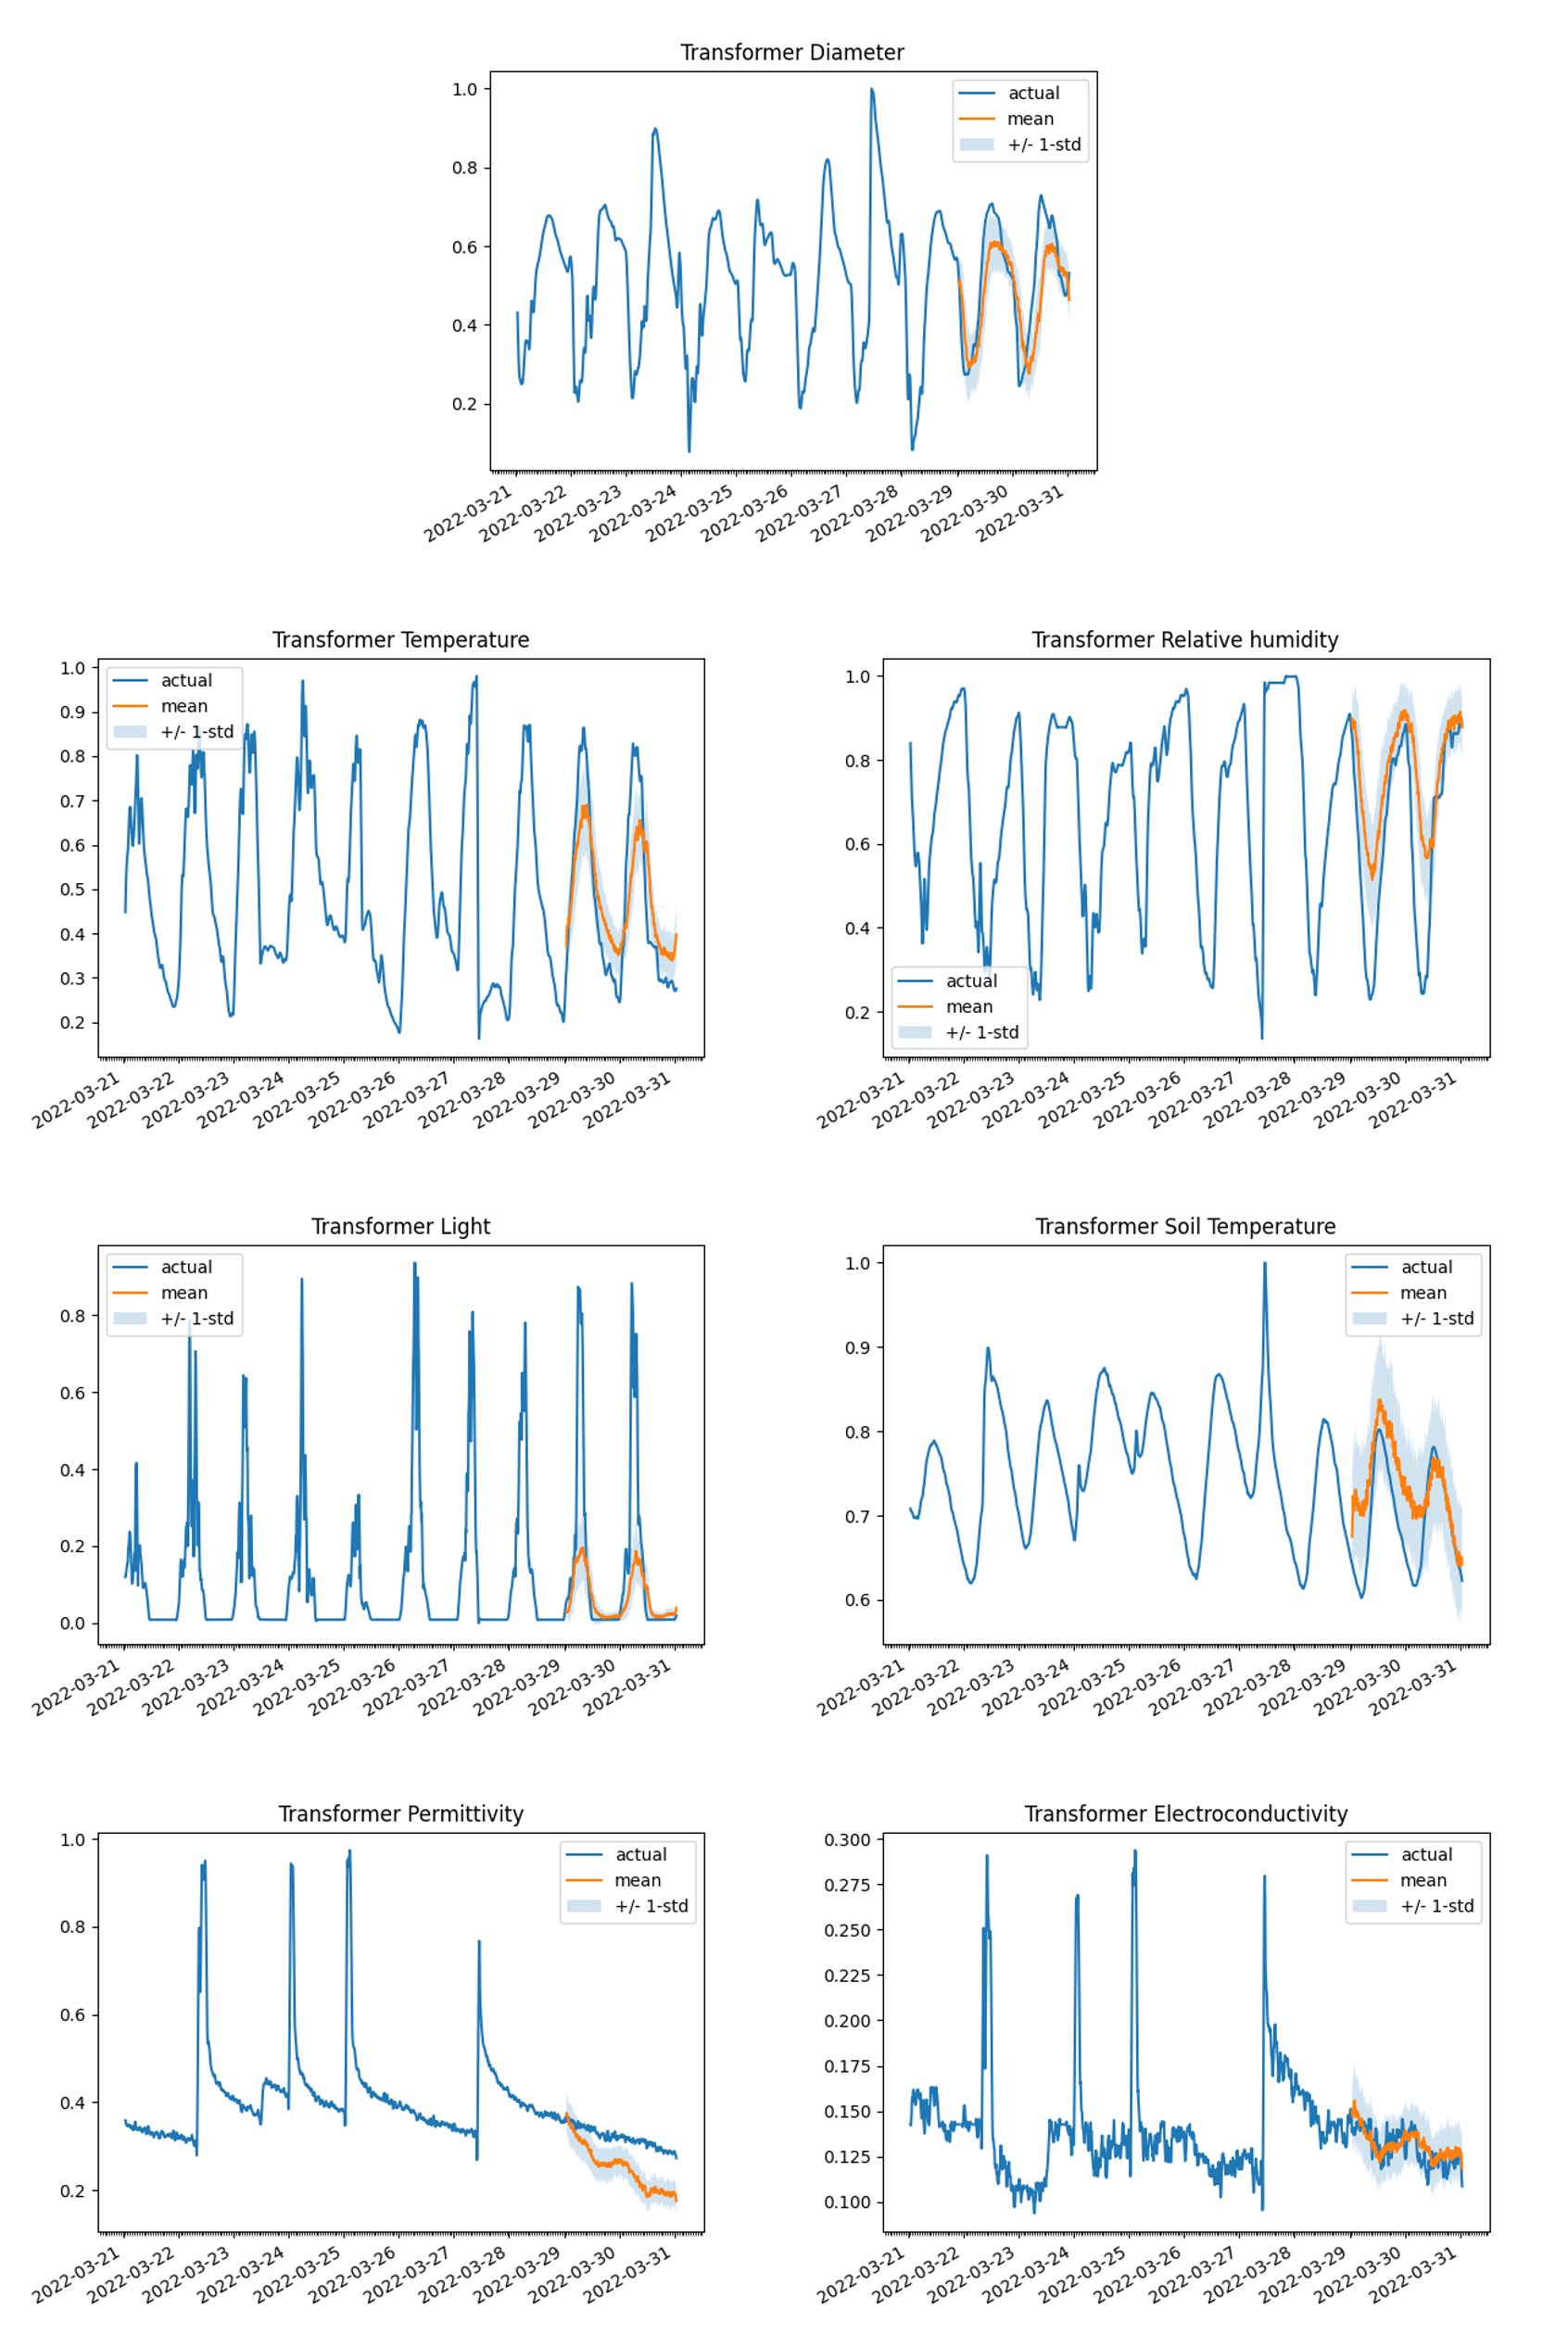
\includegraphics[width=15 cm]{6_ChapterResults/figuras/T3.png}
    \caption{Comparison between the predicted values generated by the T3 model and the actual observed values for the 7 variables over a two-day prediction horizon}
    \label{T3}
\end{figure}

\subsection{Informer}
The results for the Informer variant, as presented in Tables \ref{I1_M} and \ref{I1_R}, show similarities to those observed with the Transformer. However, unlike the Transformer, the Informer demonstrates a greater capability to handle larger Prediction Length and Context Length values more effectively. This suggests that the Informer is better suited for scenarios requiring longer forecasting horizons.

Additionally, Table \ref{I1_T} reveals a significant reduction in training time for models that work with larger datasets, such as T3, T4, T6, T7, and T8. Conversely, when the amount of data is smaller, as in models T1, T2, and T5, the training time increases. This highlights the Informer's efficiency in dealing with larger data volumes, while it may require more time when working with smaller datasets.

Figure \ref{I3} presents a comparison between the I3 model's predictions and the actual values of the 7 variables. This illustration emphasizes the I3 model's accuracy over a two-day prediction horizon, offering a clear visual insight into its performance across the variables.

\begin{table}[ht]
    \centering
    \resizebox{\textwidth}{!}{%
    \begin{tabular}{ccccccccc}
    \rowcolor[HTML]{FFFFFF} 
    \multicolumn{9}{c}{\cellcolor[HTML]{FFFFFF}\textbf{MSE   (Sorted by model)}} \\
    \rowcolor[HTML]{FFFFFF} 
    Model                      & Diameter                       & Electroconductivity            & Light                          & Permittivity                   & Relative\_humidity             & Soil\_Temperature              & Temperature                    & Mean                           \\
    \cellcolor[HTML]{FFFFFF}I1 & \cellcolor[HTML]{FA8070}-13.37 & \cellcolor[HTML]{63BE7B}-41.54 & \cellcolor[HTML]{FFE383}-11.66 & \cellcolor[HTML]{63BE7B}-34.17 & \cellcolor[HTML]{FDEA83}-11.18 & \cellcolor[HTML]{C0D880}-17.29 & \cellcolor[HTML]{FBEA83}-11.76 & \cellcolor[HTML]{DBE081}-20.14 \\
    \rowcolor[HTML]{63BE7B} 
    \cellcolor[HTML]{FFFFFF}I2 & -19.28                         & \cellcolor[HTML]{F5E883}-37.85 & -48.90                         & \cellcolor[HTML]{A7D17E}-30.25 & -27.19                         & -25.58                         & -18.46                         & -29.64                         \\
    \cellcolor[HTML]{FFFFFF}I3 & \cellcolor[HTML]{FFDF82}-14.42 & \cellcolor[HTML]{F8696B}-25.45 & \cellcolor[HTML]{FEEA83}-11.71 & \cellcolor[HTML]{F8696B}-17.95 & \cellcolor[HTML]{FAE983}-11.46 & \cellcolor[HTML]{E8E482}-13.71 & \cellcolor[HTML]{E0E282}-12.98 & \cellcolor[HTML]{F96D6C}-15.38 \\
    \cellcolor[HTML]{FFFFFF}I4 & \cellcolor[HTML]{FFDA81}-14.36 & \cellcolor[HTML]{FFDD82}-36.29 & \cellcolor[HTML]{FEEA83}-11.92 & \cellcolor[HTML]{E5E382}-26.62 & \cellcolor[HTML]{FFE583}-10.89 & \cellcolor[HTML]{F8696B}-6.04  & \cellcolor[HTML]{FDC37D}-11.00 & \cellcolor[HTML]{FDC57D}-16.73 \\
    \rowcolor[HTML]{F8696B} 
    \cellcolor[HTML]{FFFFFF}I5 & -13.12                         & \cellcolor[HTML]{FCAE79}-31.83 & -11.34                         & \cellcolor[HTML]{FED280}-23.74 & -7.91                          & \cellcolor[HTML]{FDBF7C}-9.77  & -9.64                          & -15.33                         \\
    \cellcolor[HTML]{FFFFFF}I6 & \cellcolor[HTML]{DAE081}-15.67 & \cellcolor[HTML]{FFE984}-37.37 & \cellcolor[HTML]{FECB7E}-11.60 & \cellcolor[HTML]{9ECF7E}-30.75 & \cellcolor[HTML]{FED680}-10.51 & \cellcolor[HTML]{FA8B72}-7.52  & \cellcolor[HTML]{FFE383}-11.49 & \cellcolor[HTML]{F8E983}-17.85 \\
    \cellcolor[HTML]{FFFFFF}I7 & \cellcolor[HTML]{FAE983}-14.69 & \cellcolor[HTML]{9ECF7E}-40.04 & \cellcolor[HTML]{FCA878}-11.51 & \cellcolor[HTML]{FDB57A}-22.17 & \cellcolor[HTML]{FA8070}-8.45  & \cellcolor[HTML]{FDB77A}-9.43  & \cellcolor[HTML]{FED680}-11.30 & \cellcolor[HTML]{FEC97E}-16.80 \\
    \cellcolor[HTML]{FFFFFF}I8 & \cellcolor[HTML]{9CCE7E}-17.53 & \cellcolor[HTML]{71C27B}-41.18 & \cellcolor[HTML]{FDEA83}-12.00 & \cellcolor[HTML]{FA8471}-19.44 & \cellcolor[HTML]{FBE983}-11.41 & \cellcolor[HTML]{E5E382}-14.00 & \cellcolor[HTML]{C1D980}-14.32 & \cellcolor[HTML]{EFE683}-18.55 \\
    \end{tabular}%
    }
    \caption{Mean Squared Errors (MSE) for different Informer models obtained by varying the prediction length and context length, sorted by model}
    \label{I1_M}
    \end{table}

\begin{table}[]
    \centering
    \resizebox{\textwidth}{!}{%
    \begin{tabular}{
    >{\columncolor[HTML]{FFFFFF}}c cccccccc}
    \multicolumn{9}{c}{\cellcolor[HTML]{FFFFFF}\textbf{R2 (Sorted by model)}}                                                                                                                                                                                                                                                     \\
    Model & \cellcolor[HTML]{FFFFFF}Diameter & \cellcolor[HTML]{FFFFFF}Electroconductivity & \cellcolor[HTML]{FFFFFF}Light & \cellcolor[HTML]{FFFFFF}Permittivity & \cellcolor[HTML]{FFFFFF}Relative\_humidity & \cellcolor[HTML]{FFFFFF}Soil\_Temperature & \cellcolor[HTML]{FFFFFF}Temperature & \cellcolor[HTML]{FFFFFF}Mean   \\
    I1    & \cellcolor[HTML]{F97D6E}-1.10    & \cellcolor[HTML]{82C77D}-0.14               & \cellcolor[HTML]{FEEA83}-0.26 & \cellcolor[HTML]{6DC17C}-1.32        & \cellcolor[HTML]{F3E884}-0.45              & \cellcolor[HTML]{8BCA7E}-4.85             & \cellcolor[HTML]{E9E583}-0.72       & \cellcolor[HTML]{63BE7B}-1.26  \\
    I2    & \cellcolor[HTML]{FEDB81}-0.66    & \cellcolor[HTML]{FDCF7E}-7.95               & \cellcolor[HTML]{F8696B}-3.67 & \cellcolor[HTML]{FEDC81}-12.95       & \cellcolor[HTML]{63BE7B}0.61               & \cellcolor[HTML]{63BE7B}-0.17             & \cellcolor[HTML]{F8696B}-8.10       & \cellcolor[HTML]{C7DB81}-4.70  \\
    I3    & \cellcolor[HTML]{FEE081}-0.63    & \cellcolor[HTML]{F8696B}-34.12              & \cellcolor[HTML]{B8D780}-0.18 & \cellcolor[HTML]{F8696B}-34.00       & \cellcolor[HTML]{EEE784}-0.41              & \cellcolor[HTML]{B9D780}-10.32            & \cellcolor[HTML]{9ECF7F}-0.29       & \cellcolor[HTML]{F8696B}-11.42 \\
    I4    & \cellcolor[HTML]{C5DB81}-0.29    & \cellcolor[HTML]{D6E082}-0.70               & \cellcolor[HTML]{FEEA83}-0.25 & \cellcolor[HTML]{63BE7B}-0.76        & \cellcolor[HTML]{FEE382}-0.63              & \cellcolor[HTML]{F8696B}-59.17            & \cellcolor[HTML]{FEE983}-0.91       & \cellcolor[HTML]{FBAC77}-8.96  \\
    I5    & \cellcolor[HTML]{F8696B}-1.20    & \cellcolor[HTML]{FDD37F}-7.08               & \cellcolor[HTML]{FEE983}-0.28 & \cellcolor[HTML]{DFE283}-8.24        & \cellcolor[HTML]{F8696B}-2.20              & \cellcolor[HTML]{FDD07E}-27.03            & \cellcolor[HTML]{FEDA80}-1.77       & \cellcolor[HTML]{FEE683}-6.83  \\
    I6    & \cellcolor[HTML]{B8D780}-0.22    & \cellcolor[HTML]{FEE983}-1.26               & \cellcolor[HTML]{D8E082}-0.21 & \cellcolor[HTML]{65BF7C}-0.84        & \cellcolor[HTML]{FED980}-0.76              & \cellcolor[HTML]{FA9373}-46.07            & \cellcolor[HTML]{F9EA84}-0.81       & \cellcolor[HTML]{FEDC81}-7.17  \\
    I7    & \cellcolor[HTML]{F6E984}-0.53    & \cellcolor[HTML]{8ECB7E}-0.22               & \cellcolor[HTML]{F5E884}-0.23 & \cellcolor[HTML]{FEE081}-12.24       & \cellcolor[HTML]{F98670}-1.83              & \cellcolor[HTML]{FDC87D}-29.34            & \cellcolor[HTML]{FEEA83}-0.89       & \cellcolor[HTML]{FAEA84}-6.47  \\
    I8    & \cellcolor[HTML]{63BE7B}0.20     & \cellcolor[HTML]{63BE7B}0.06                & \cellcolor[HTML]{63BE7B}-0.10 & \cellcolor[HTML]{FAA075}-23.83       & \cellcolor[HTML]{F1E784}-0.43              & \cellcolor[HTML]{B3D580}-9.58             & \cellcolor[HTML]{63BE7B}0.06        & \cellcolor[HTML]{CADC81}-4.80 
    \end{tabular}%
    }
    \caption{R-squared (R²) for different Informer models obtained by varying the prediction length and context length, sorted by model}
    \label{I1_R}
    \end{table}


\begin{table}[]
    \begin{tabular}{
    >{\columncolor[HTML]{FFFFFF}}c cc
    >{\columncolor[HTML]{FFFFFF}}c c}
    \multicolumn{2}{c}{\cellcolor[HTML]{FFFFFF}\textbf{Training   Time (Sorted by model)}} & \cellcolor[HTML]{FFFFFF} & \multicolumn{2}{c}{\cellcolor[HTML]{FFFFFF}\textbf{Training Time (Sorted   by training time)}} \\
    Model                  & \cellcolor[HTML]{FFFFFF}Training time {[}s{]}                 & \cellcolor[HTML]{FFFFFF} & Model                      & \cellcolor[HTML]{FFFFFF}Training time {[}s{]}                     \\
    I1                     & \cellcolor[HTML]{FECC7F}148.62                                &                          & I2                         & \cellcolor[HTML]{63BE7B}113.54                                    \\
    I2                     & \cellcolor[HTML]{63BE7B}113.54                                &                          & I6                         & \cellcolor[HTML]{BDD880}129.43                                    \\
    I3                     & \cellcolor[HTML]{D3DE81}133.22                                &                          & I3                         & \cellcolor[HTML]{D3DE81}133.22                                    \\
    I4                     & \cellcolor[HTML]{F8696B}173.61                                &                          & I5                         & \cellcolor[HTML]{F4E883}138.98                                    \\
    I5                     & \cellcolor[HTML]{F4E883}138.98                                &                          & I7                         & \cellcolor[HTML]{FFE483}142.6                                     \\
    I6                     & \cellcolor[HTML]{BDD880}129.43                                &                          & I1                         & \cellcolor[HTML]{FECC7F}148.62                                    \\
    I7                     & \cellcolor[HTML]{FFE483}142.6                                 &                          & I8                         & \cellcolor[HTML]{FDC47D}150.68                                    \\
    I8                     & \cellcolor[HTML]{FDC47D}150.68                                &                          & I4                         & \cellcolor[HTML]{F8696B}173.61                                   
    \end{tabular}%
    \caption{Training times for different Informer models obtained by varying the prediction length and context length, sorted by model and training time values}
    \label{I1_T}
    \end{table}

\begin{figure}[htbp]
    \centering
    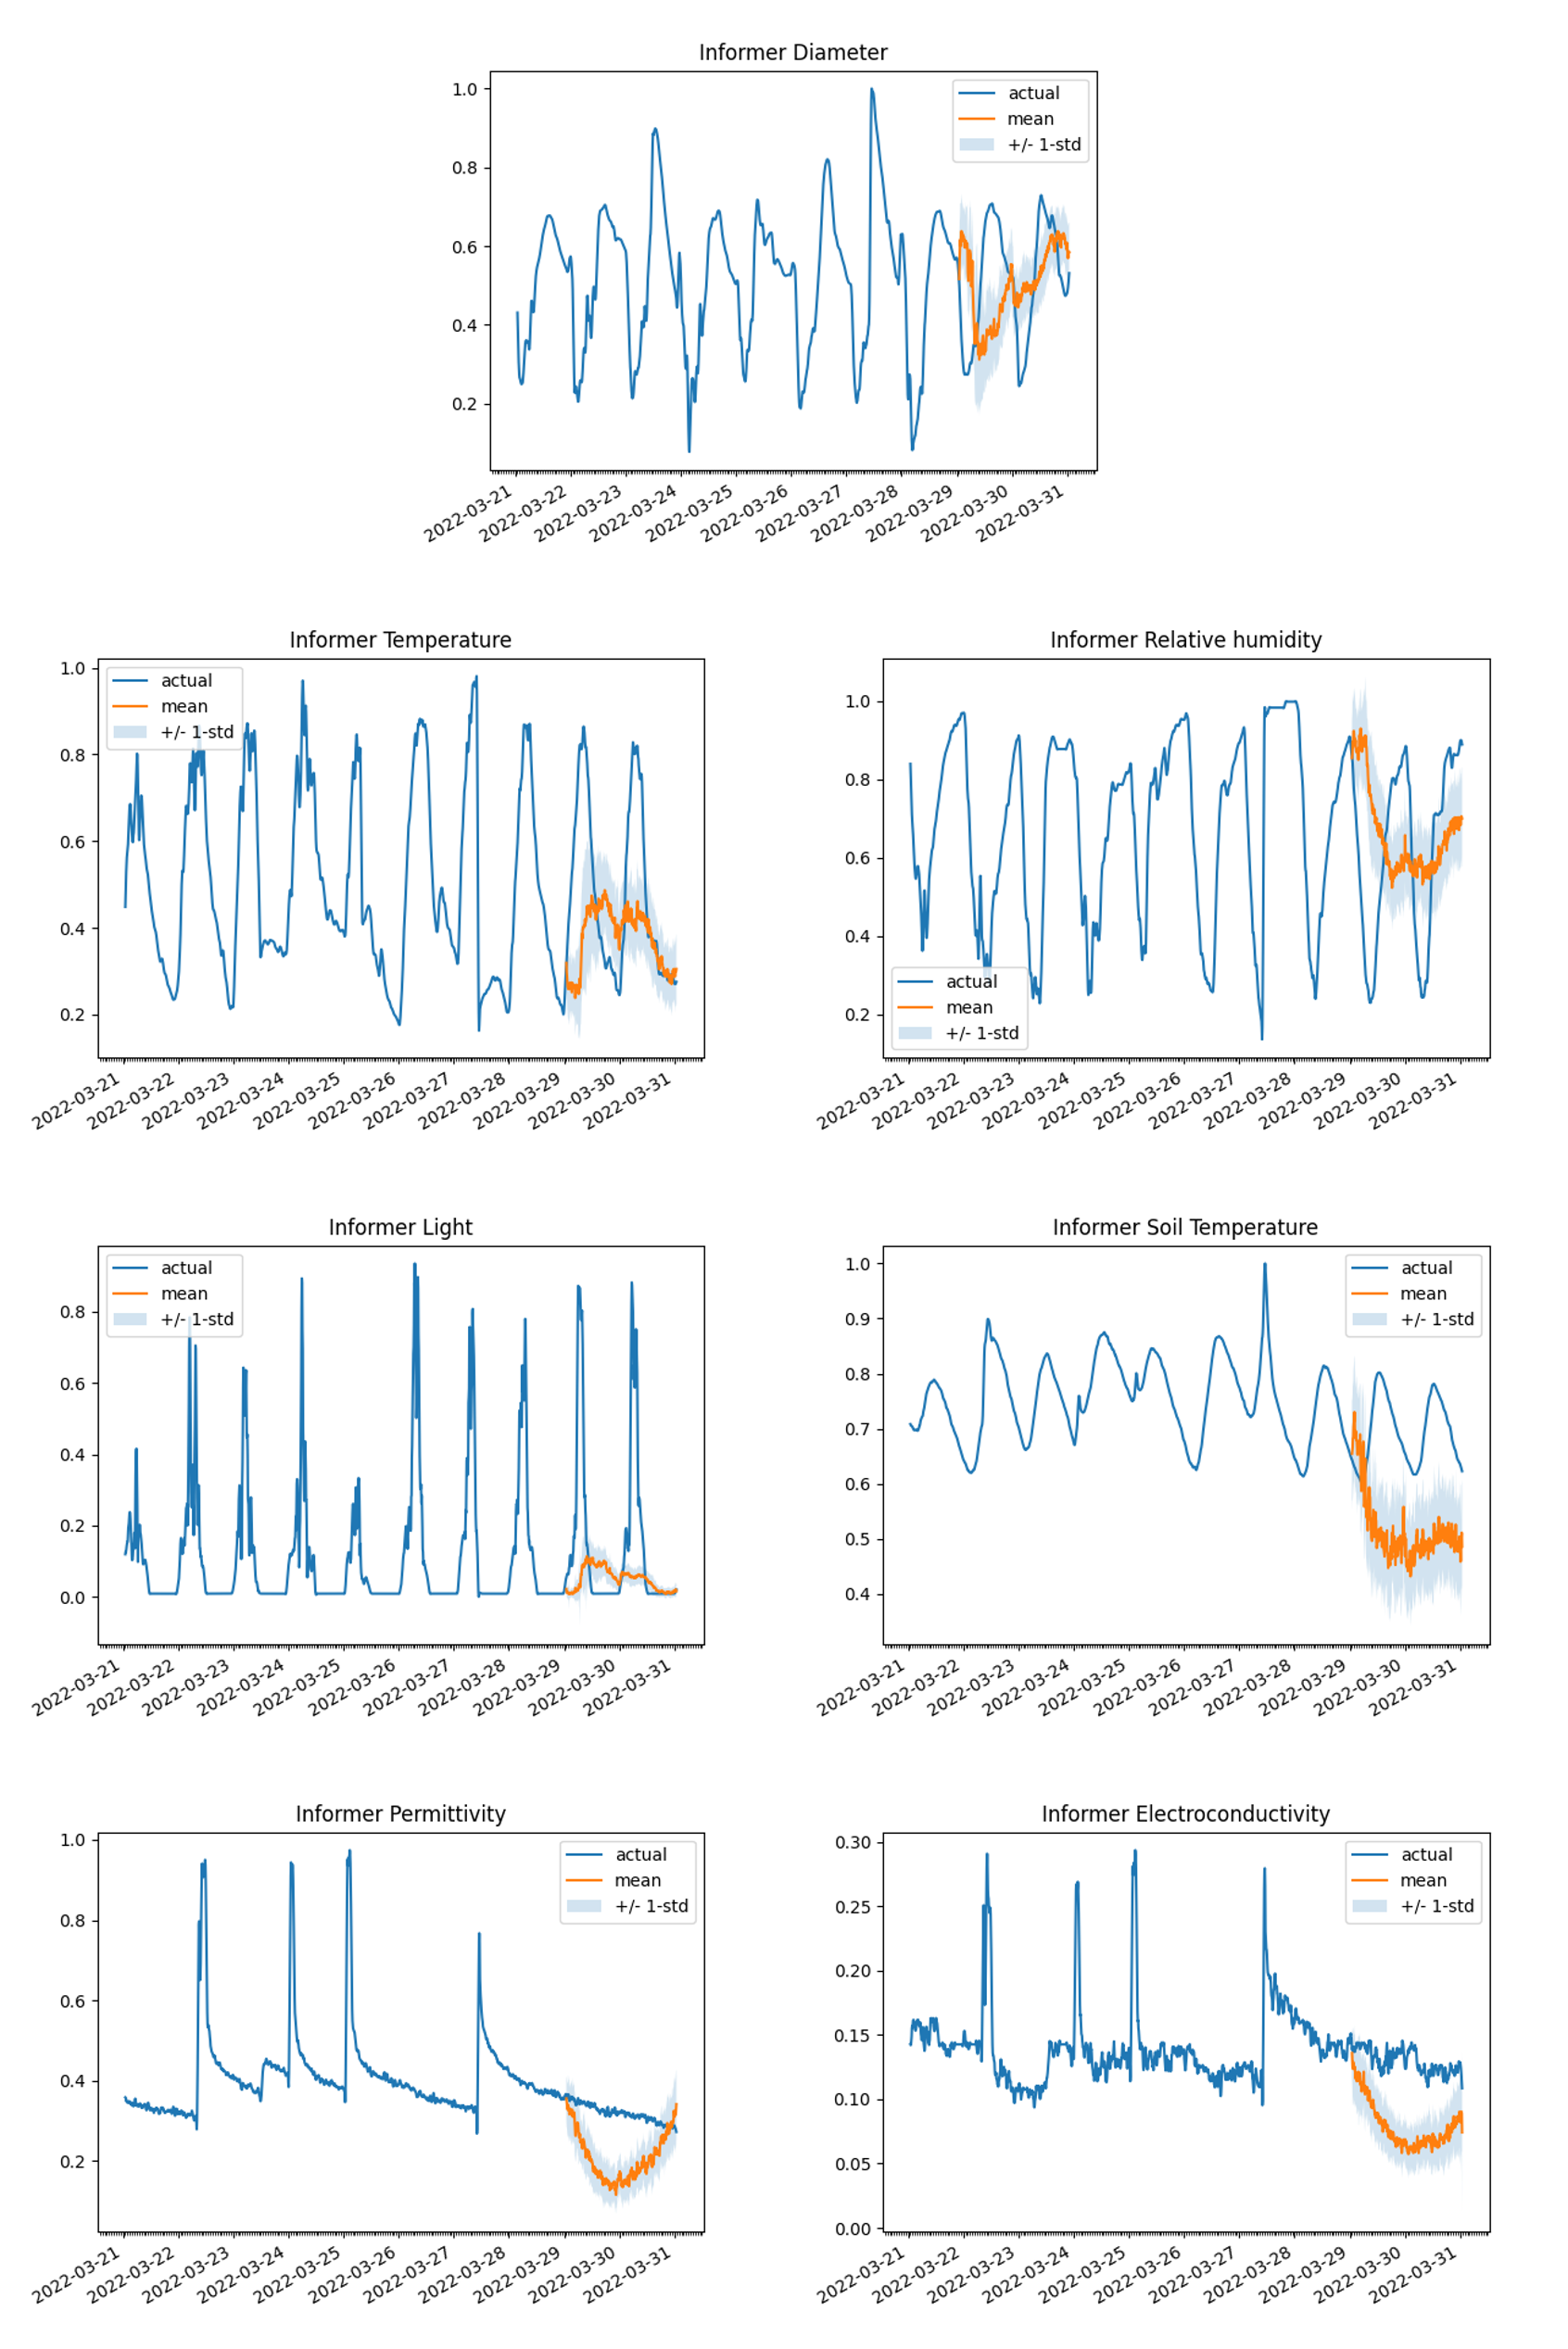
\includegraphics[width=15 cm]{6_ChapterResults/figuras/I3.png}
    \caption{Comparison between the predicted values generated by the I3 model and the actual observed values for the 7 variables over a two-day prediction horizon}
    \label{I3}
\end{figure}


\subsection{Autoformer}
The results for the Autoformer variant, as shown in Tables \ref{A1_M} and \ref{A1_R}, indicate better performance than the Transformer when more data is used, similar to the Informer. This demonstrates the Autoformer's strong scalability and ability to effectively manage larger Prediction Length and Context Length values.

Additionally, as seen in Table \ref{A1_T}, the Autoformer, like the Informer, is more efficient in terms of training time compared to the Transformer when working with large datasets. However, it's important to note that the Autoformer is not more efficient than the Informer in any of its models. Therefore, when comparing the three variants, the Informer stands out as the most computationally efficient model.

In Figure \ref{A3}, the predictions of the A3 model are compared with the actual observed values for the 7 variables. The figure demonstrates the model's precision over a two-day prediction period, providing a clear visual assessment of its performance across different variables.

\begin{table}[]
    \centering
    \resizebox{\textwidth}{!}{%
    \begin{tabular}{ccccccccc}
    \rowcolor[HTML]{FFFFFF} 
    \multicolumn{9}{c}{\cellcolor[HTML]{FFFFFF}\textbf{MSE   (Sorted by model)}}                                                                                                                                                                                                                       \\
    \rowcolor[HTML]{FFFFFF} 
    Model                      & Diameter                       & Electroconductivity            & Light                          & Permittivity                   & Relative\_humidity             & Soil\_Temperature              & Temperature                    & Mean                           \\
    \cellcolor[HTML]{FFFFFF}A1 & \cellcolor[HTML]{FEC97E}-20.51 & \cellcolor[HTML]{63BE7B}-40.48 & \cellcolor[HTML]{FCEA83}-11.84 & \cellcolor[HTML]{91CB7D}-37.39 & \cellcolor[HTML]{E0E282}-20.16 & \cellcolor[HTML]{6FC17B}-21.57 & \cellcolor[HTML]{FFE884}-21.91 & \cellcolor[HTML]{D4DE81}-24.84 \\
    \cellcolor[HTML]{FFFFFF}A2 & \cellcolor[HTML]{FA8170}-17.36 & \cellcolor[HTML]{B5D57F}-38.79 & \cellcolor[HTML]{63BE7B}-45.94 & \cellcolor[HTML]{63BE7B}-42.25 & \cellcolor[HTML]{63BE7B}-29.24 & \cellcolor[HTML]{FEEA83}-19.53 & \cellcolor[HTML]{FECF7F}-20.41 & \cellcolor[HTML]{63BE7B}-30.50 \\
    \cellcolor[HTML]{FFFFFF}A3 & \cellcolor[HTML]{63BE7B}-25.42 & \cellcolor[HTML]{FDBE7C}-35.20 & \cellcolor[HTML]{FEEA83}-11.44 & \cellcolor[HTML]{FAE983}-26.30 & \cellcolor[HTML]{FFEB84}-17.98 & \cellcolor[HTML]{63BE7B}-21.75 & \cellcolor[HTML]{6FC17B}-24.59 & \cellcolor[HTML]{F4E883}-23.24 \\
    \cellcolor[HTML]{FFFFFF}A4 & \cellcolor[HTML]{FFDA81}-21.25 & \cellcolor[HTML]{F8696B}-31.40 & \cellcolor[HTML]{FDEA83}-11.62 & \cellcolor[HTML]{FB8F73}-22.73 & \cellcolor[HTML]{F9E983}-18.41 & \cellcolor[HTML]{FAE983}-19.59 & \cellcolor[HTML]{8FCA7D}-24.03 & \cellcolor[HTML]{FDC27C}-21.29 \\
    \cellcolor[HTML]{FFFFFF}A5 & \cellcolor[HTML]{85C77C}-24.68 & \cellcolor[HTML]{95CC7D}-39.44 & \cellcolor[HTML]{FCAA78}-11.27 & \cellcolor[HTML]{FFE884}-25.68 & \cellcolor[HTML]{FED881}-17.00 & \cellcolor[HTML]{FFEB84}-19.52 & \cellcolor[HTML]{F3E783}-22.30 & \cellcolor[HTML]{FCEA83}-22.84 \\
    \cellcolor[HTML]{FFFFFF}A6 & \cellcolor[HTML]{DAE081}-22.83 & \cellcolor[HTML]{F1E783}-37.54 & \cellcolor[HTML]{FCAE79}-11.27 & \cellcolor[HTML]{FDEA83}-25.95 & \cellcolor[HTML]{FFEB84}-17.95 & \cellcolor[HTML]{FBA076}-18.12 & \cellcolor[HTML]{63BE7B}-24.81 & \cellcolor[HTML]{FFE984}-22.64 \\
    \rowcolor[HTML]{F8696B} 
    \cellcolor[HTML]{FFFFFF}A7 & -16.30                         & \cellcolor[HTML]{FECE7F}-35.93 & \cellcolor[HTML]{F9726D}-11.19 & -21.49                         & -11.42                         & -17.12                         & -14.34                         & -18.25                         \\
    \cellcolor[HTML]{FFFFFF}A8 & \cellcolor[HTML]{D5DF81}-22.94 & \cellcolor[HTML]{FFE583}-36.97 & \cellcolor[HTML]{F8696B}-11.18 & \cellcolor[HTML]{F9706D}-21.71 & \cellcolor[HTML]{FEEA83}-18.00 & \cellcolor[HTML]{FCA577}-18.22 & \cellcolor[HTML]{FED981}-20.99 & \cellcolor[HTML]{FDC67D}-21.43
    \end{tabular}%
    }
    \caption{Mean Squared Errors (MSE) for different Autoformer models obtained by varying the prediction length and context length, sorted by model}
    \label{A1_M}
    \end{table}


\begin{table}[]
    \centering
    \resizebox{\textwidth}{!}{%
    \begin{tabular}{ccccccccc}
    \rowcolor[HTML]{FFFFFF} 
    \multicolumn{9}{c}{\cellcolor[HTML]{FFFFFF}\textbf{R2 (Sorted by model)}}                                                                                                                                                                                                                  \\
    \rowcolor[HTML]{FFFFFF} 
    Model                      & Diameter                      & Electroconductivity           & Light                         & Permittivity                   & Relative\_humidity            & Soil\_Temperature             & Temperature                  & Mean                          \\
    \cellcolor[HTML]{FFFFFF}A1 & \cellcolor[HTML]{FEE282}0.59  & \cellcolor[HTML]{69C07C}-0.45 & \cellcolor[HTML]{63BE7B}-0.21 & \cellcolor[HTML]{6BC17C}-0.11  & \cellcolor[HTML]{63BE7B}0.82  & \cellcolor[HTML]{88C97E}-1.18 & \cellcolor[HTML]{FEEA83}0.83 & \cellcolor[HTML]{63BE7B}0.04  \\
    \rowcolor[HTML]{F8696B} 
    \cellcolor[HTML]{FFFFFF}A2 & -1.58                         & -6.21                         & -8.24                         & \cellcolor[HTML]{63BE7B}0.12   & \cellcolor[HTML]{A9D27F}0.76  & \cellcolor[HTML]{F98C71}-3.70 & -4.80                        & -3.38                         \\
    \cellcolor[HTML]{FFFFFF}A3 & \cellcolor[HTML]{63BE7B}0.87  & \cellcolor[HTML]{FDCF7E}-2.73 & \cellcolor[HTML]{A3D17F}-0.25 & \cellcolor[HTML]{F8E984}-4.12  & \cellcolor[HTML]{FEEA83}0.69  & \cellcolor[HTML]{63BE7B}-0.78 & \cellcolor[HTML]{6EC27C}0.91 & \cellcolor[HTML]{DEE283}-0.77 \\
    \cellcolor[HTML]{FFFFFF}A4 & \cellcolor[HTML]{FEEA83}0.74  & \cellcolor[HTML]{FBA276}-4.26 & \cellcolor[HTML]{FEEA83}-0.34 & \cellcolor[HTML]{DCE182}-3.32  & \cellcolor[HTML]{E1E383}0.71  & \cellcolor[HTML]{B4D680}-1.66 & \cellcolor[HTML]{7BC57D}0.91 & \cellcolor[HTML]{FEE983}-1.03 \\
    \cellcolor[HTML]{FFFFFF}A5 & \cellcolor[HTML]{84C87D}0.85  & \cellcolor[HTML]{63BE7B}-0.40 & \cellcolor[HTML]{EFE784}-0.31 & \cellcolor[HTML]{FEE382}-4.90  & \cellcolor[HTML]{FEE182}0.61  & \cellcolor[HTML]{D1DE82}-1.97 & \cellcolor[HTML]{EFE784}0.85 & \cellcolor[HTML]{DBE182}-0.75 \\
    \cellcolor[HTML]{FFFFFF}A6 & \cellcolor[HTML]{EDE683}0.77  & \cellcolor[HTML]{B8D780}-1.17 & \cellcolor[HTML]{ECE683}-0.30 & \cellcolor[HTML]{FEE883}-4.55  & \cellcolor[HTML]{FEEA83}0.68  & \cellcolor[HTML]{FCBB7A}-3.10 & \cellcolor[HTML]{63BE7B}0.92 & \cellcolor[HTML]{FBEA84}-0.97 \\
    \cellcolor[HTML]{FFFFFF}A7 & \cellcolor[HTML]{FCBD7B}-0.06 & \cellcolor[HTML]{FEE182}-2.15 & \cellcolor[HTML]{FEEA83}-0.33 & \cellcolor[HTML]{F8696B}-14.51 & \cellcolor[HTML]{F8696B}-0.43 & \cellcolor[HTML]{F8696B}-4.16 & \cellcolor[HTML]{FED880}0.06 & \cellcolor[HTML]{F8796E}-3.08 \\
    \cellcolor[HTML]{FFFFFF}A8 & \cellcolor[HTML]{E5E483}0.77  & \cellcolor[HTML]{DAE182}-1.47 & \cellcolor[HTML]{FEEA83}-0.33 & \cellcolor[HTML]{F8736C}-13.72 & \cellcolor[HTML]{FEEB84}0.69  & \cellcolor[HTML]{FCC37C}-3.00 & \cellcolor[HTML]{FEE983}0.80 & \cellcolor[HTML]{FBA276}-2.33
    \end{tabular}%
    }
    \caption{R-squared (R²) for different Autoformer models obtained by varying the prediction length and context length, sorted by model}
    \label{A1_R}
    \end{table}


\begin{table}[]
    \begin{tabular}{
    >{\columncolor[HTML]{FFFFFF}}c cc
    >{\columncolor[HTML]{FFFFFF}}c c}
    \multicolumn{2}{c}{\cellcolor[HTML]{FFFFFF}\textbf{Training   Time (Sorted by model)}} & \cellcolor[HTML]{FFFFFF} & \multicolumn{2}{c}{\cellcolor[HTML]{FFFFFF}\textbf{Training Time (Sorted   by training time)}} \\
    Model                  & \cellcolor[HTML]{FFFFFF}Training time {[}s{]}                 & \cellcolor[HTML]{FFFFFF} & Model                      & \cellcolor[HTML]{FFFFFF}Training time {[}s{]}                     \\
    A1                     & \cellcolor[HTML]{85C77C}268.74                                &                          & A2                         & \cellcolor[HTML]{63BE7B}263.36                                    \\
    A2                     & \cellcolor[HTML]{63BE7B}263.36                                &                          & A1                         & \cellcolor[HTML]{85C77C}268.74                                    \\
    A3                     & \cellcolor[HTML]{FFE784}290.26                                &                          & A5                         & \cellcolor[HTML]{D8DF81}281.66                                    \\
    A4                     & \cellcolor[HTML]{F8696B}372.63                                &                          & A6                         & \cellcolor[HTML]{EDE683}284.96                                    \\
    A5                     & \cellcolor[HTML]{D8DF81}281.66                                &                          & A3                         & \cellcolor[HTML]{FFE784}290.26                                    \\
    A6                     & \cellcolor[HTML]{EDE683}284.96                                &                          & A7                         & \cellcolor[HTML]{FCB079}326.78                                    \\
    A7                     & \cellcolor[HTML]{FCB079}326.78                                &                          & A8                         & \cellcolor[HTML]{FB9373}345.52                                    \\
    A8                     & \cellcolor[HTML]{FB9373}345.52                                &                          & A4                         & \cellcolor[HTML]{F8696B}372.63                                   
    \end{tabular}%
    \caption{Training times for different Autoformer models obtained by varying the prediction length and context length, sorted by model and training time values}
    \label{A1_T}
    \end{table}

\begin{figure}[htbp]
    \centering
    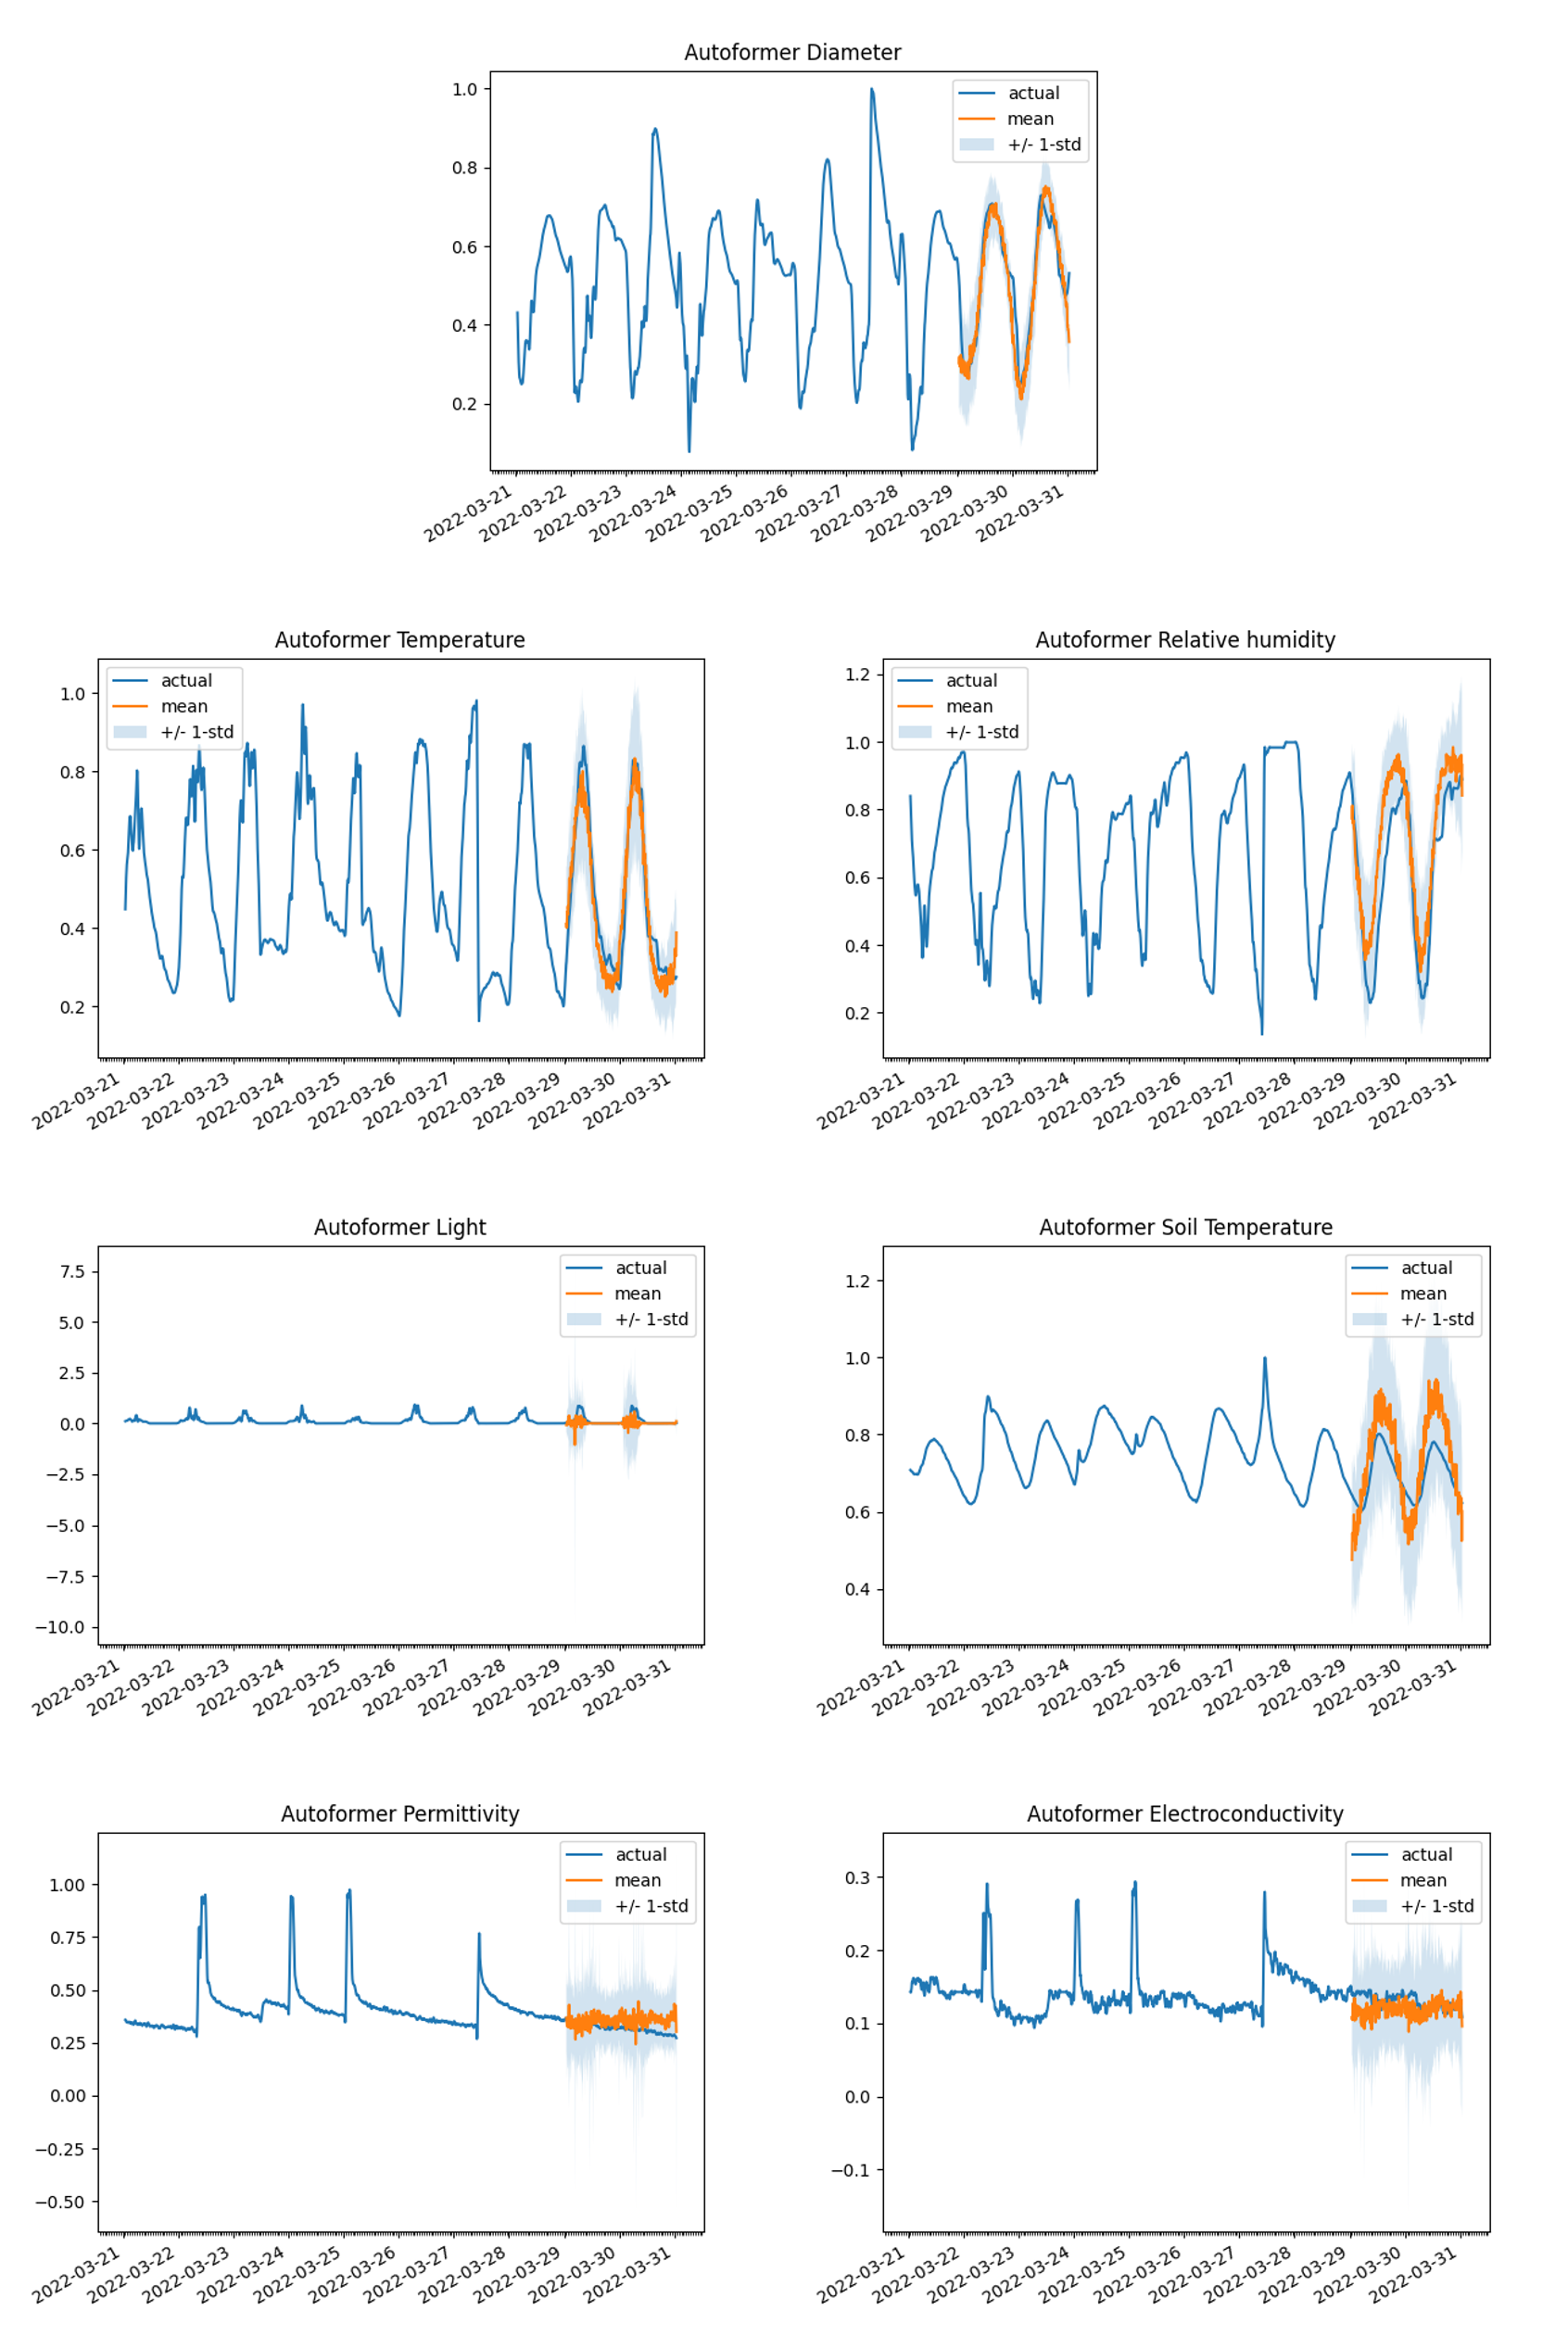
\includegraphics[width=15 cm]{6_ChapterResults/figuras/A3.png}
    \caption{Comparison between the predicted values generated by the A3 model and the actual observed values for the 7 variables over a two-day prediction horizon}
    \label{A3}
\end{figure}






\section{Effect of Lags Sequence}
In this section, we advance to the next phase of experimentation by focusing on models T3, I3, and A3, which were identified as the most practical in the previous phase. Here, we test these models with different values of Lags sequence to evaluate how variations in the lagged input data affect their predictive performance. This analysis aims to determine the optimal lag configuration that enhances model accuracy and utility, further refining our approach to time series forecasting.

\subsection{Transformer}
The results for the Transformer variant with added Lags Sequences, as shown in Tables \ref{T2_M} and \ref{T2_R}, indicate mixed outcomes. Compared to the original T3 model, which did not use any Lags Sequence, the performance deteriorates for models T9, T10, and T11. However, the results improve for models T12 and T13, suggesting that while smaller Lags Sequences might not be beneficial, a sufficiently large Lags Sequence can enhance the Transformer's predictive capabilities. Among all the models tested so far, we consider T13 to be the best, primarily due to its strong performance in predicting plant diameter.Figure \ref{T13} illustrates the comparison between the predictions generated by the T13 model and the actual observed values, highlighting the model's effectiveness.

On the other hand, as seen in Table \ref{T2_T}, the addition of Lags Sequences leads to increased training times, as working with Lags Sequences requires additional comparisons, resulting in a higher computational cost.


\begin{table}[]
    \centering
    \resizebox{\textwidth}{!}{%
    \begin{tabular}{ccccccccc}
    \rowcolor[HTML]{FFFFFF} 
    \multicolumn{9}{c}{\cellcolor[HTML]{FFFFFF}\textbf{MSE   (Sorted by model)}}                                                                                                                                                                                                                        \\
    \rowcolor[HTML]{FFFFFF} 
    Model                       & Diameter                       & Electroconductivity            & Light                          & Permittivity                   & Relative Humidity              & Soil Temperature               & Temperature                    & Mean                           \\
    \cellcolor[HTML]{FFFFFF}T9  & \cellcolor[HTML]{FB9D75}-17.25 & \cellcolor[HTML]{9FCF7E}-31.89 & \cellcolor[HTML]{FFEB84}-14.01 & \cellcolor[HTML]{F8696B}-17.64 & \cellcolor[HTML]{63BE7B}-14.98 & \cellcolor[HTML]{F96F6D}-12.27 & \cellcolor[HTML]{63BE7B}-18.33 & \cellcolor[HTML]{FFDD82}-18.05 \\
    \cellcolor[HTML]{FFFFFF}T10 & \cellcolor[HTML]{FFEB84}-19.55 & \cellcolor[HTML]{F8696B}-25.03 & \cellcolor[HTML]{FA8270}-13.33 & \cellcolor[HTML]{63BE7B}-31.58 & \cellcolor[HTML]{FFEB84}-14.16 & \cellcolor[HTML]{63BE7B}-22.43 & \cellcolor[HTML]{FFEB84}-16.63 & \cellcolor[HTML]{72C27B}-20.39 \\
    \rowcolor[HTML]{F8696B} 
    \cellcolor[HTML]{FFFFFF}T11 & -15.73                         & \cellcolor[HTML]{FFEB84}-27.28 & -13.18                         & \cellcolor[HTML]{FFEB84}-24.94 & -11.28                         & \cellcolor[HTML]{FFEB84}-16.59 & -15.22                         & -17.74                         \\
    \cellcolor[HTML]{FFFFFF}T12 & \cellcolor[HTML]{88C87D}-21.92 & \cellcolor[HTML]{63BE7B}-34.80 & \cellcolor[HTML]{63BE7B}-14.11 & \cellcolor[HTML]{C0D880}-27.61 & \cellcolor[HTML]{FECD7F}-13.49 & \cellcolor[HTML]{ECE582}-17.30 & \cellcolor[HTML]{F96A6C}-15.23 & \cellcolor[HTML]{63BE7B}-20.64 \\
    \cellcolor[HTML]{FFFFFF}T13 & \cellcolor[HTML]{63BE7B}-22.65 & \cellcolor[HTML]{F9766E}-25.25 & \cellcolor[HTML]{ABD27F}-14.06 & \cellcolor[HTML]{FCAC78}-21.35 & \cellcolor[HTML]{DAE081}-14.35 & \cellcolor[HTML]{F8696B}-12.06 & \cellcolor[HTML]{E3E382}-16.92 & \cellcolor[HTML]{FFEB84}-18.09
    \end{tabular}%
    }
    \caption{Mean Squared Errors (MSE) for different Transformer models obtained by varying the Lags Sequence values, sorted by model}
    \label{T2_M}
    \end{table}

\begin{table}[]
    \centering
    \resizebox{\textwidth}{!}{%
    \begin{tabular}{ccccccccc}
    \rowcolor[HTML]{FFFFFF} 
    \multicolumn{9}{c}{\cellcolor[HTML]{FFFFFF}\textbf{R2 (Sorted by model)}}                                                                                                                                                                                                                    \\
    \rowcolor[HTML]{FFFFFF} 
    Model                       & Diameter                      & Electroconductivity            & Light                        & Permittivity                   & Relative\_humidity            & Soil\_Temperature              & Temperature                  & Mean                          \\
    \cellcolor[HTML]{FFFFFF}T9  & \cellcolor[HTML]{FBAA77}0.15  & \cellcolor[HTML]{83C87D}-6.98  & \cellcolor[HTML]{FFEB84}0.31 & \cellcolor[HTML]{F8696B}-36.60 & \cellcolor[HTML]{63BE7B}0.37  & \cellcolor[HTML]{F8726C}-14.78 & \cellcolor[HTML]{63BE7B}0.63 & \cellcolor[HTML]{F98D72}-8.13 \\
    \cellcolor[HTML]{FFFFFF}T10 & \cellcolor[HTML]{FFEB84}0.50  & \cellcolor[HTML]{F8696B}-37.71 & \cellcolor[HTML]{F9826F}0.19 & \cellcolor[HTML]{63BE7B}-0.52  & \cellcolor[HTML]{FFEB84}0.24  & \cellcolor[HTML]{63BE7B}-0.52  & \cellcolor[HTML]{FFEB84}0.45 & \cellcolor[HTML]{FFEB84}-5.34 \\
    \cellcolor[HTML]{FFFFFF}T11 & \cellcolor[HTML]{F8696B}-0.21 & \cellcolor[HTML]{FFEB84}-22.07 & \cellcolor[HTML]{F8696B}0.16 & \cellcolor[HTML]{FFEB84}-6.00  & \cellcolor[HTML]{F8696B}-0.47 & \cellcolor[HTML]{FFEB84}-4.83  & \cellcolor[HTML]{F8696B}0.23 & \cellcolor[HTML]{E9E583}-4.74 \\
    \cellcolor[HTML]{FFFFFF}T12 & \cellcolor[HTML]{7FC67D}0.71  & \cellcolor[HTML]{63BE7B}-3.08  & \cellcolor[HTML]{63BE7B}0.32 & \cellcolor[HTML]{A4D17F}-2.79  & \cellcolor[HTML]{FDD47F}0.12  & \cellcolor[HTML]{E0E283}-3.96  & \cellcolor[HTML]{F86A6B}0.23 & \cellcolor[HTML]{63BE7B}-1.21 \\
    \cellcolor[HTML]{FFFFFF}T13 & \cellcolor[HTML]{63BE7B}0.76  & \cellcolor[HTML]{F8786E}-35.83 & \cellcolor[HTML]{A8D27F}0.32 & \cellcolor[HTML]{FCC47C}-15.01 & \cellcolor[HTML]{D8E082}0.27  & \cellcolor[HTML]{F8696B}-15.53 & \cellcolor[HTML]{DFE283}0.48 & \cellcolor[HTML]{F8696B}-9.22
    \end{tabular}%
    }
    \caption{R-squared (R²) for different Transformer models obtained by varying the Lags Sequence values, sorted by model}
    \label{T2_R}
    \end{table}


\begin{table}[]
    \begin{tabular}{ccccc}
    \multicolumn{2}{c}{\cellcolor[HTML]{FFFFFF}\textbf{Training   Time (Sorted by model)}} &  & \multicolumn{2}{c}{\cellcolor[HTML]{FFFFFF}\textbf{Training Time (Sorted   by training time)}} \\
    Model                         & Training time {[}s{]}                                  &  & Model                             & Training time {[}s{]}                                      \\
    T9                            & \cellcolor[HTML]{63BE7B}246.61                         &  & T9                                & \cellcolor[HTML]{63BE7B}246.61                             \\
    T10                           & \cellcolor[HTML]{E5E382}255.4                          &  & T10                               & \cellcolor[HTML]{E5E382}255.4                              \\
    T11                           & \cellcolor[HTML]{F8696B}260.8                          &  & T13                               & \cellcolor[HTML]{FFEB84}257.08                             \\
    T12                           & \cellcolor[HTML]{FFEA84}257.13                         &  & T12                               & \cellcolor[HTML]{FFEA84}257.13                             \\
    T13                           & \cellcolor[HTML]{FFEB84}257.08                         &  & T11                               & \cellcolor[HTML]{F8696B}260.8                             
    \end{tabular}%
    \caption{Training times for different Transformer models obtained  by varying the Lags Sequence values, sorted by model and training time values}
    \label{T2_T}
    \end{table}

\begin{figure}[htbp]
    \centering
    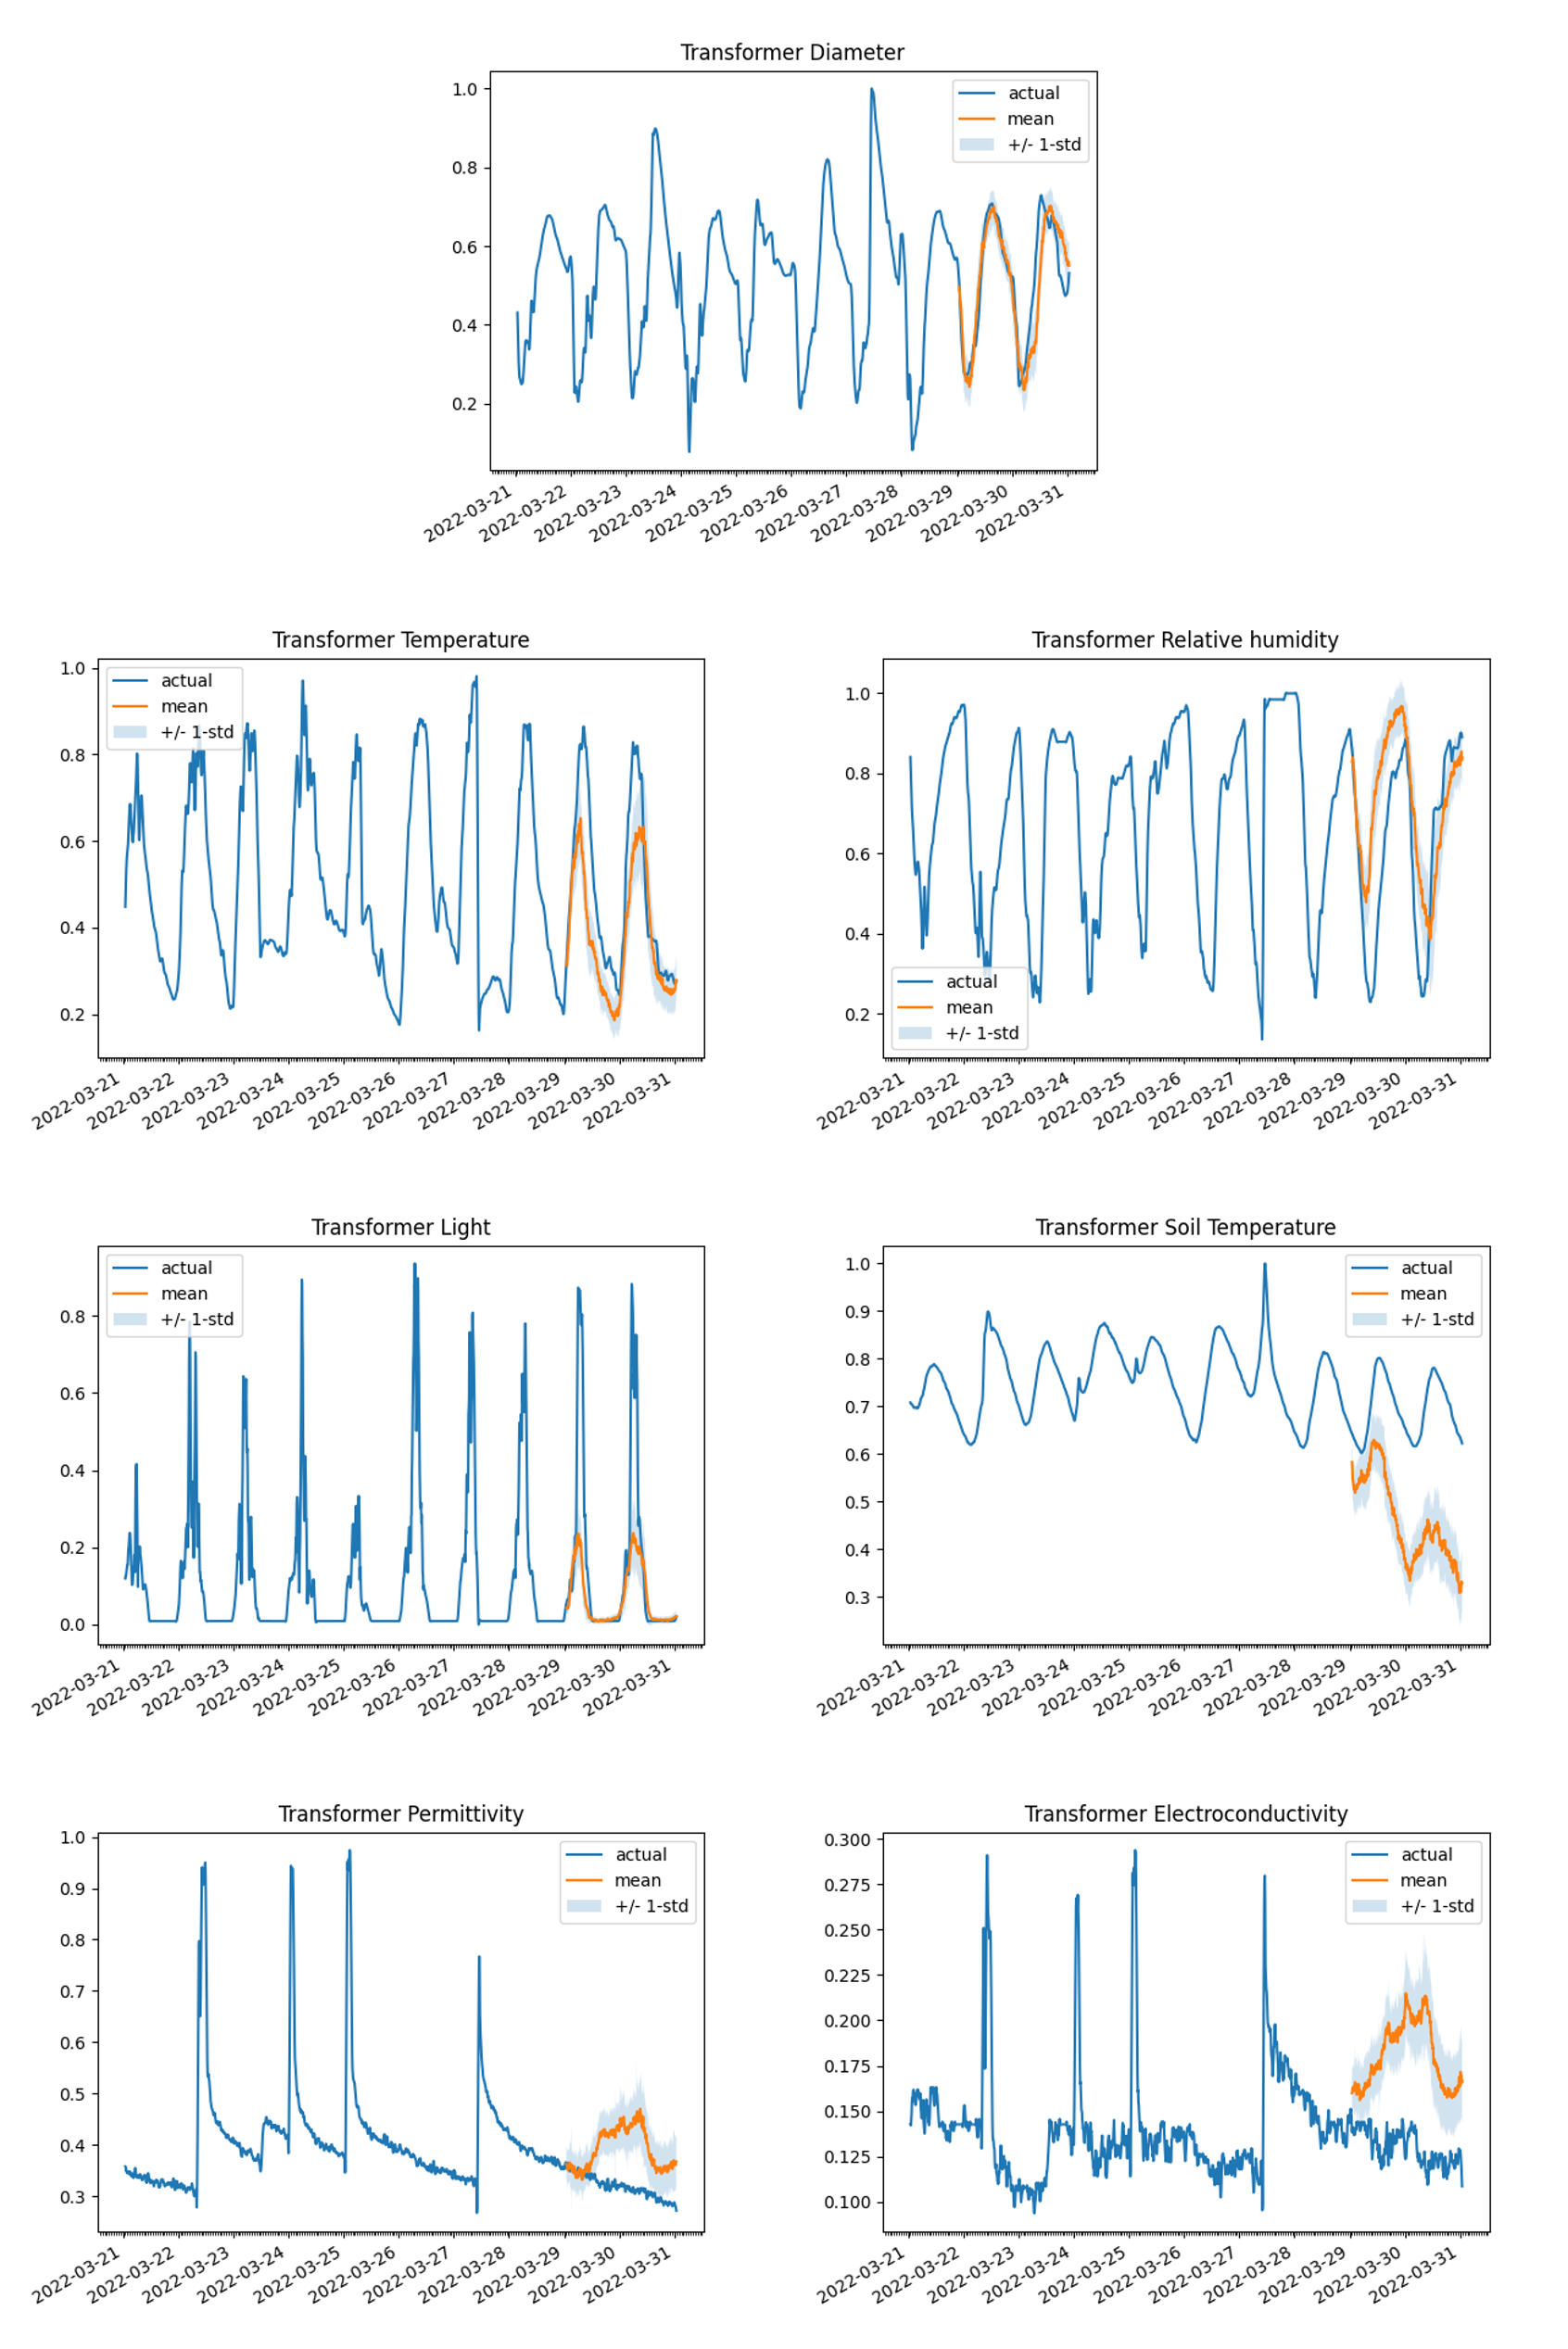
\includegraphics[width=15 cm]{6_ChapterResults/figuras/T13.png}
    \caption{Comparison between the predicted values generated by the T13 model and the actual observed values for the 7 variables over a two-day prediction horizon}
    \label{T13}
\end{figure}
    

\subsection{Informer}
The results for the Informer variant with added Lags Sequences, as shown in Tables \ref{I2_M} and \ref{I2_R}, demonstrate an improvement across all models compared to the original I3 model, which did not use any Lags Sequence. Each model that incorporates Lags Sequences shows better performance, indicating that this approach is beneficial for the Informer architecture. Once again, I13 has been chosen as the best overall model, not only for its strong performance in predicting plant diameter but also for its accuracy in forecasting other variables. Figure \ref{I13} illustrates the comparison between the predictions generated by the I13 model and the actual observed values, highlighting the model's effectiveness.

Additionally, as seen in Table \ref{I2_T}, the Informer variant proves to be more computationally efficient than the Transformer, reducing training times even with the added complexity of Lags Sequences.

\begin{table}[]
    \centering
    \resizebox{\textwidth}{!}{%
    \begin{tabular}{ccccccccc}
    \multicolumn{9}{c}{\textbf{MSE   (Sorted by model)}}                                                                                                                                                                                                                          \\
    Model & Diameter                       & Electroconductivity            & Light                          & Permittivity                   & Relative\_humidity             & Soil\_Temperature              & Temperature                    & Mean                           \\
    I9    & \cellcolor[HTML]{F8696B}-17.16 & \cellcolor[HTML]{FFEB84}-29.00 & \cellcolor[HTML]{FFEB84}-12.54 & \cellcolor[HTML]{FDBB7B}-17.83 & \cellcolor[HTML]{FFEB84}-11.75 & \cellcolor[HTML]{FB9073}-11.63 & \cellcolor[HTML]{75C37C}-15.37 & \cellcolor[HTML]{F8696B}-16.47 \\
    I10   & \cellcolor[HTML]{CBDC81}-20.80 & \cellcolor[HTML]{FFEB84}-29.01 & \cellcolor[HTML]{63BE7B}-13.14 & \cellcolor[HTML]{F8696B}-17.25 & \cellcolor[HTML]{FDBC7B}-11.24 & \cellcolor[HTML]{FFEB84}-15.74 & \cellcolor[HTML]{63BE7B}-15.40 & \cellcolor[HTML]{FCB37A}-17.51 \\
    I11   & \cellcolor[HTML]{FFEB84}-20.70 & \cellcolor[HTML]{F8696B}-24.60 & \cellcolor[HTML]{FFDC82}-12.49 & \cellcolor[HTML]{9DCE7E}-25.99 & \cellcolor[HTML]{63BE7B}-12.61 & \cellcolor[HTML]{E7E482}-16.73 & \cellcolor[HTML]{FFEB84}-15.16 & \cellcolor[HTML]{FFEB84}-18.32 \\
    I12   & \cellcolor[HTML]{63BE7B}-21.01 & \cellcolor[HTML]{91CB7D}-34.80 & \cellcolor[HTML]{D5DF81}-12.70 & \cellcolor[HTML]{63BE7B}-30.64 & \cellcolor[HTML]{B2D47F}-12.17 & \cellcolor[HTML]{F8696B}-9.89  & \cellcolor[HTML]{F8696B}-11.77 & \cellcolor[HTML]{63BE7B}-19.00 \\
    I13   & \cellcolor[HTML]{FBA076}-18.64 & \cellcolor[HTML]{63BE7B}-37.29 & \cellcolor[HTML]{F8696B}-12.05 & \cellcolor[HTML]{FFEB84}-18.17 & \cellcolor[HTML]{F8696B}-10.35 & \cellcolor[HTML]{63BE7B}-22.38 & \cellcolor[HTML]{FCA878}-13.41 & \cellcolor[HTML]{79C47C}-18.90
    \end{tabular}%
    }
    \caption{Mean Squared Errors (MSE) for different Informer models obtained by varying the Lags Sequence values, sorted by model}
    \label{I2_M}
    \end{table}

\begin{table}[]
    \centering
    \resizebox{\textwidth}{!}{%
    \begin{tabular}{ccccccccc}
    \multicolumn{9}{c}{\textbf{R2 (Sorted by model)}}                                                                                                                                                                                                                       \\
    Model & Diameter                     & Electroconductivity            & Light                         & Permittivity                   & Relative\_humidity            & Soil\_Temperature              & Temperature                   & Mean                          \\
    I9    & \cellcolor[HTML]{F8696B}0.13 & \cellcolor[HTML]{FEEA83}-14.51 & \cellcolor[HTML]{FFEB84}0.03  & \cellcolor[HTML]{FCBD7B}-35.01 & \cellcolor[HTML]{FFEB84}-0.32 & \cellcolor[HTML]{FBA276}-17.29 & \cellcolor[HTML]{76C47D}0.26  & \cellcolor[HTML]{F8696B}-9.53 \\
    I10   & \cellcolor[HTML]{C9DC81}0.63 & \cellcolor[HTML]{FFEB84}-14.49 & \cellcolor[HTML]{63BE7B}0.15  & \cellcolor[HTML]{F8696B}-40.09 & \cellcolor[HTML]{FCC07B}-0.49 & \cellcolor[HTML]{FFEB84}-6.09  & \cellcolor[HTML]{63BE7B}0.26  & \cellcolor[HTML]{FA9C74}-8.59 \\
    I11   & \cellcolor[HTML]{FFEB84}0.62 & \cellcolor[HTML]{F8696B}-41.77 & \cellcolor[HTML]{FEDC81}0.01  & \cellcolor[HTML]{75C47D}-4.49  & \cellcolor[HTML]{63BE7B}-0.09 & \cellcolor[HTML]{D7E082}-4.65  & \cellcolor[HTML]{FFEB84}0.22  & \cellcolor[HTML]{FFEB84}-7.16 \\
    I12   & \cellcolor[HTML]{63BE7B}0.64 & \cellcolor[HTML]{79C57D}-3.08  & \cellcolor[HTML]{D4DF82}0.06  & \cellcolor[HTML]{63BE7B}-0.88  & \cellcolor[HTML]{AFD480}-0.20 & \cellcolor[HTML]{F8696B}-26.30 & \cellcolor[HTML]{F8696B}-0.70 & \cellcolor[HTML]{63BE7B}-4.35 \\
    I13   & \cellcolor[HTML]{FBAC77}0.38 & \cellcolor[HTML]{63BE7B}-1.30  & \cellcolor[HTML]{F8696B}-0.09 & \cellcolor[HTML]{FFEB84}-32.31 & \cellcolor[HTML]{F8696B}-0.83 & \cellcolor[HTML]{63BE7B}-0.54  & \cellcolor[HTML]{FCB479}-0.16 & \cellcolor[HTML]{86C97E}-4.98
    \end{tabular}%
    }
    \caption{R-squared (R²) for different Informer models obtained by varying the Lags Sequence values, sorted by model}
    \label{I2_R}
    \end{table}


\begin{table}[]
    \begin{tabular}{ccccc}
    \multicolumn{2}{c}{\textbf{Training   Time (Sorted by model)}} &  & \multicolumn{2}{c}{\textbf{Training Time (Sorted   by training time)}} \\
    Model             & Training time {[}s{]}                      &  & Model                 & Training time {[}s{]}                          \\
    I9                & \cellcolor[HTML]{63BE7B}128.38             &  & I9                    & \cellcolor[HTML]{63BE7B}128.38                 \\
    I10               & \cellcolor[HTML]{FB9374}149.6              &  & I10                   & \cellcolor[HTML]{FB9374}149.6                  \\
    I11               & \cellcolor[HTML]{F8696B}154.53             &  & I11                   & \cellcolor[HTML]{F8696B}154.53                 \\
    I12               & \cellcolor[HTML]{A4D07E}132.9              &  & I12                   & \cellcolor[HTML]{A4D07E}132.9                  \\
    I13               & \cellcolor[HTML]{FFEB84}139.2              &  & I13                   & \cellcolor[HTML]{FFEB84}139.2                 
    \end{tabular}
    \caption{Training times for different Informer models obtained  by varying the Lags Sequence values, sorted by model and training time values}
    \label{I2_T}
    \end{table}

\begin{figure}[htbp]
    \centering
    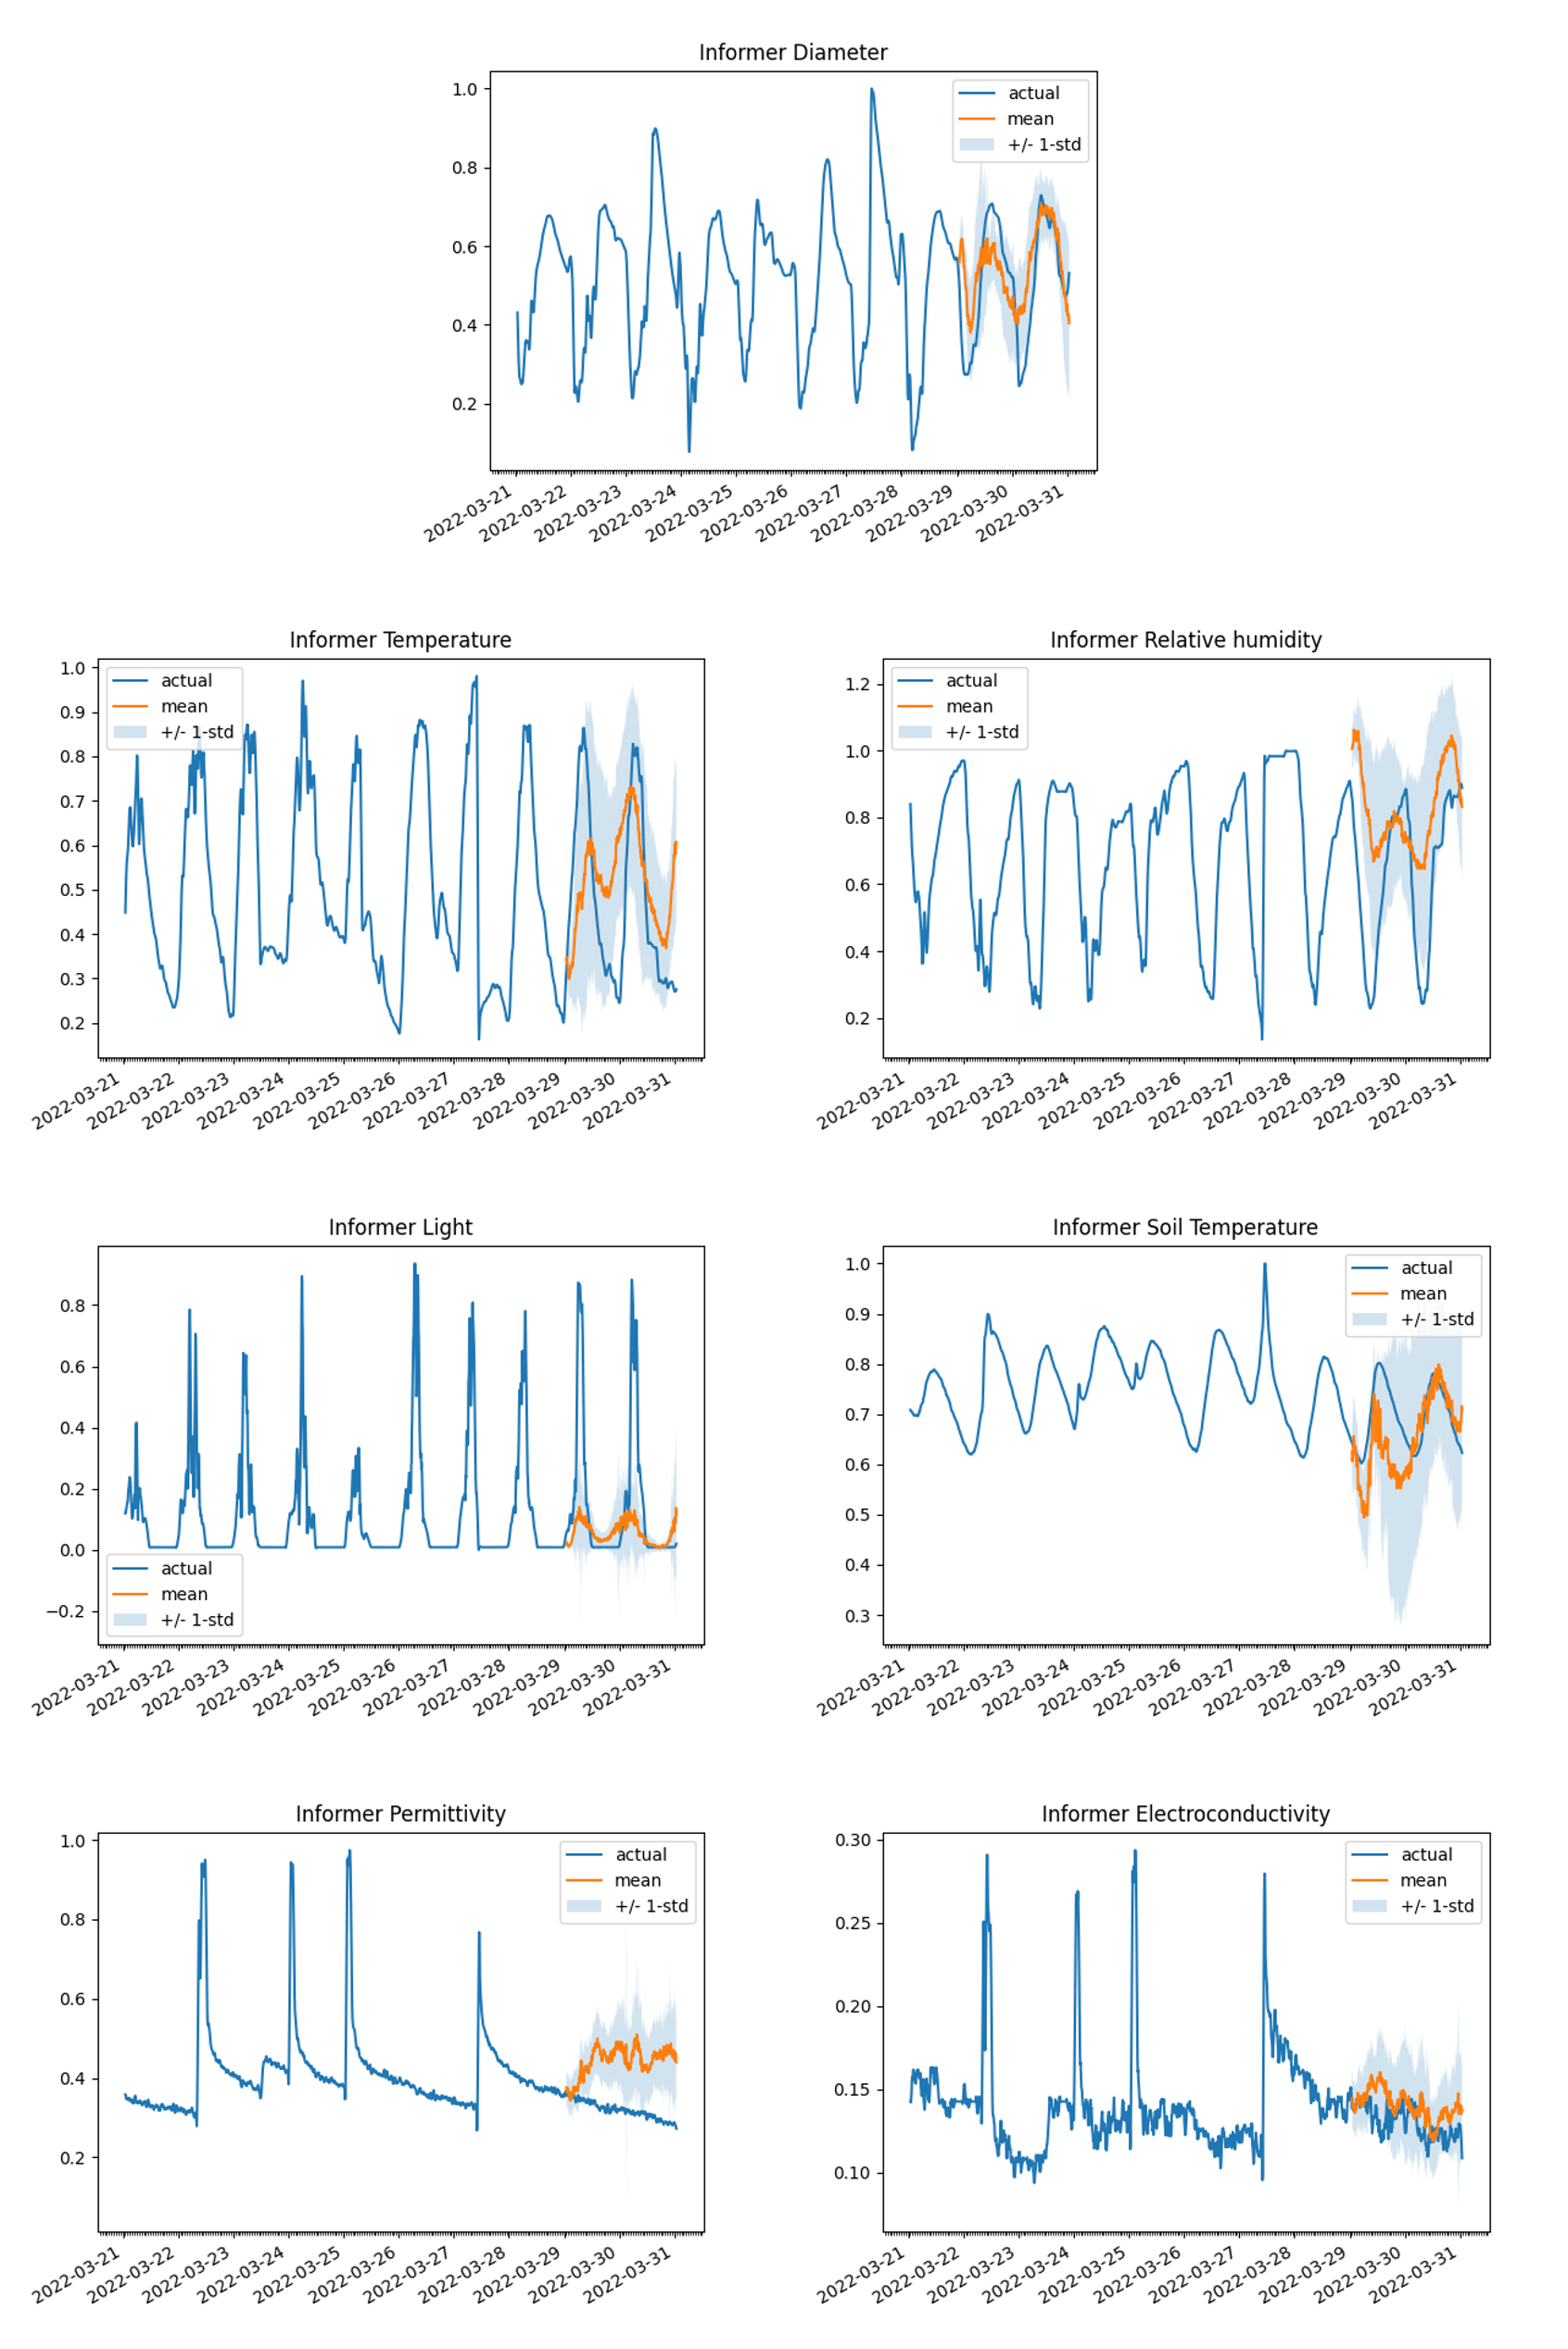
\includegraphics[width=15 cm]{6_ChapterResults/figuras/I13.png}
    \caption{Comparison between the predicted values generated by the I13 model and the actual observed values for the 7 variables over a two-day prediction horizon}
    \label{I13}
\end{figure}

\subsection{Autoformer}
The results for the Autoformer variant with added Lags Sequences, as shown in Tables \ref{A2_M} and \ref{A2_R}, reveal a significant improvement compared to the original A3 model, which did not utilize any Lags Sequence. This enhancement is particularly notable in the prediction of environmental variables, demonstrating the effectiveness of Lags Sequences in boosting the model's overall accuracy. Among the models tested, A11 is considered the best so far, due to its superior performance across key metrics. Figure \ref{A11} illustrates the comparison between the predictions generated by the A11 model and the actual observed values, highlighting the model's effectiveness.

However, as observed in Table \ref{A2_T}, there is an increase in computational cost, similar to what was seen with the Transformer and Informer variants. The addition of Lags Sequences requires more computational resources, leading to longer training times.


\begin{table}[]
    \centering
    \resizebox{\textwidth}{!}{%
    \begin{tabular}{ccccccccc}
    \multicolumn{9}{c}{\textbf{MSE   (Sorted by model)}}                                                                                                                                                                                                                          \\
    Model & Diameter                       & Electroconductivity            & Light                          & Permittivity                   & Relative\_humidity             & Soil\_Temperature              & Temperature                    & Mean                           \\
    A9    & \cellcolor[HTML]{63BE7B}-25.58 & \cellcolor[HTML]{FFEB84}-36.22 & \cellcolor[HTML]{FB9C75}-11.17 & \cellcolor[HTML]{FFEB84}-22.81 & \cellcolor[HTML]{FDC07C}-17.45 & \cellcolor[HTML]{FCA276}-20.25 & \cellcolor[HTML]{C4DA80}-22.55 & \cellcolor[HTML]{FFEB84}-22.29 \\
    A10   & \cellcolor[HTML]{FFEB84}-24.50 & \cellcolor[HTML]{94CC7D}-38.19 & \cellcolor[HTML]{F8696B}-11.10 & \cellcolor[HTML]{63BE7B}-24.76 & \cellcolor[HTML]{F8696B}-16.62 & \cellcolor[HTML]{F8696B}-20.06 & \cellcolor[HTML]{F8696B}-21.00 & \cellcolor[HTML]{F9E983}-22.32 \\
    A11   & \cellcolor[HTML]{D1DD81}-24.81 & \cellcolor[HTML]{63BE7B}-39.10 & \cellcolor[HTML]{FFEB84}-11.27 & \cellcolor[HTML]{8BC97D}-24.25 & \cellcolor[HTML]{63BE7B}-18.67 & \cellcolor[HTML]{63BE7B}-21.70 & \cellcolor[HTML]{FDB67A}-21.38 & \cellcolor[HTML]{63BE7B}-23.03 \\
    A12   & \cellcolor[HTML]{FB9E76}-23.22 & \cellcolor[HTML]{FCAF79}-32.57 & \cellcolor[HTML]{63BE7B}-11.38 & \cellcolor[HTML]{FB9E76}-20.65 & \cellcolor[HTML]{FFEB84}-17.87 & \cellcolor[HTML]{FFEB84}-20.49 & \cellcolor[HTML]{63BE7B}-24.07 & \cellcolor[HTML]{FCB37A}-21.47 \\
    A13   & \cellcolor[HTML]{F8696B}-22.35 & \cellcolor[HTML]{F8696B}-28.35 & \cellcolor[HTML]{A8D27F}-11.33 & \cellcolor[HTML]{F8696B}-19.21 & \cellcolor[HTML]{88C87D}-18.48 & \cellcolor[HTML]{88C87D}-21.41 & \cellcolor[HTML]{FFEB84}-21.64 & \cellcolor[HTML]{F8696B}-20.40
    \end{tabular}%
    }
    \caption{Mean Squared Errors (MSE) for different Autoformer models obtained by varying the Lags Sequence values, sorted by model}
    \label{A2_M}
    \end{table}

\begin{table}[]
    \centering
    \resizebox{\textwidth}{!}{%
    \begin{tabular}{ccccccccc}
    \multicolumn{9}{c}{\textbf{R2 (Sorted by model)}}                                                                                                                                                                                                                    \\
    Model & Diameter                     & Electroconductivity            & Light                         & Permittivity                   & Relative\_humidity           & Soil\_Temperature             & Temperature                  & Mean                          \\
    A9    & \cellcolor[HTML]{63BE7B}0.88 & \cellcolor[HTML]{FFEB84}-1.94  & \cellcolor[HTML]{FA9C74}-0.34 & \cellcolor[HTML]{FFEB84}-10.44 & \cellcolor[HTML]{FCC37C}0.64 & \cellcolor[HTML]{FBA376}-1.51 & \cellcolor[HTML]{BBD881}0.86 & \cellcolor[HTML]{FFEB84}-1.69 \\
    A10   & \cellcolor[HTML]{FFEB84}0.84 & \cellcolor[HTML]{8ACA7E}-0.87  & \cellcolor[HTML]{F8696B}-0.36 & \cellcolor[HTML]{63BE7B}-6.30  & \cellcolor[HTML]{F8696B}0.57 & \cellcolor[HTML]{F8696B}-1.62 & \cellcolor[HTML]{F8696B}0.80 & \cellcolor[HTML]{72C37C}-0.99 \\
    A11   & \cellcolor[HTML]{CEDD82}0.85 & \cellcolor[HTML]{63BE7B}-0.52  & \cellcolor[HTML]{FFEB84}-0.30 & \cellcolor[HTML]{85C87D}-7.20  & \cellcolor[HTML]{63BE7B}0.73 & \cellcolor[HTML]{63BE7B}-0.80 & \cellcolor[HTML]{FCB77A}0.81 & \cellcolor[HTML]{63BE7B}-0.92 \\
    A12   & \cellcolor[HTML]{FBA476}0.79 & \cellcolor[HTML]{FDC97D}-5.82  & \cellcolor[HTML]{63BE7B}-0.27 & \cellcolor[HTML]{FBAA77}-17.79 & \cellcolor[HTML]{FFEB84}0.68 & \cellcolor[HTML]{FFEB84}-1.38 & \cellcolor[HTML]{63BE7B}0.90 & \cellcolor[HTML]{FCBA7A}-3.27 \\
    A13   & \cellcolor[HTML]{F8696B}0.74 & \cellcolor[HTML]{F8696B}-17.02 & \cellcolor[HTML]{A8D27F}-0.29 & \cellcolor[HTML]{F8696B}-25.21 & \cellcolor[HTML]{88C97E}0.72 & \cellcolor[HTML]{85C87D}-0.92 & \cellcolor[HTML]{FFEB84}0.83 & \cellcolor[HTML]{F8696B}-5.88
    \end{tabular}%
    }
    \caption{R-squared (R²) for different Autoformer models obtained by varying the Lags Sequence values, sorted by model}
    \label{A2_R}
    \end{table}


\begin{table}[]
    \begin{tabular}{ccccc}
    \multicolumn{2}{c}{\textbf{Training   Time (Sorted by model)}} &  & \multicolumn{2}{c}{\textbf{Training Time (Sorted   by training time)}} \\
    Model             & Training time {[}s{]}                      &  & Model                 & Training time {[}s{]}                          \\
    A9                & \cellcolor[HTML]{63BE7B}299.49             &  & A9                    & \cellcolor[HTML]{63BE7B}299.49                 \\
    A10               & \cellcolor[HTML]{CEDD81}307.03             &  & A10                   & \cellcolor[HTML]{CEDD81}307.03                 \\
    A11               & \cellcolor[HTML]{F8696B}321.64             &  & A13                   & \cellcolor[HTML]{FFEB84}310.43                 \\
    A12               & \cellcolor[HTML]{FFEA84}310.6              &  & A12                   & \cellcolor[HTML]{FFEA84}310.6                  \\
    A13               & \cellcolor[HTML]{FFEB84}310.43             &  & A11                   & \cellcolor[HTML]{F8696B}321.64                
    \end{tabular}
    \caption{Training times for different Autoformer models obtained  by varying the Lags Sequence values, sorted by model and training time values}
    \label{A2_T}
    \end{table}


\begin{figure}[htbp]
    \centering
    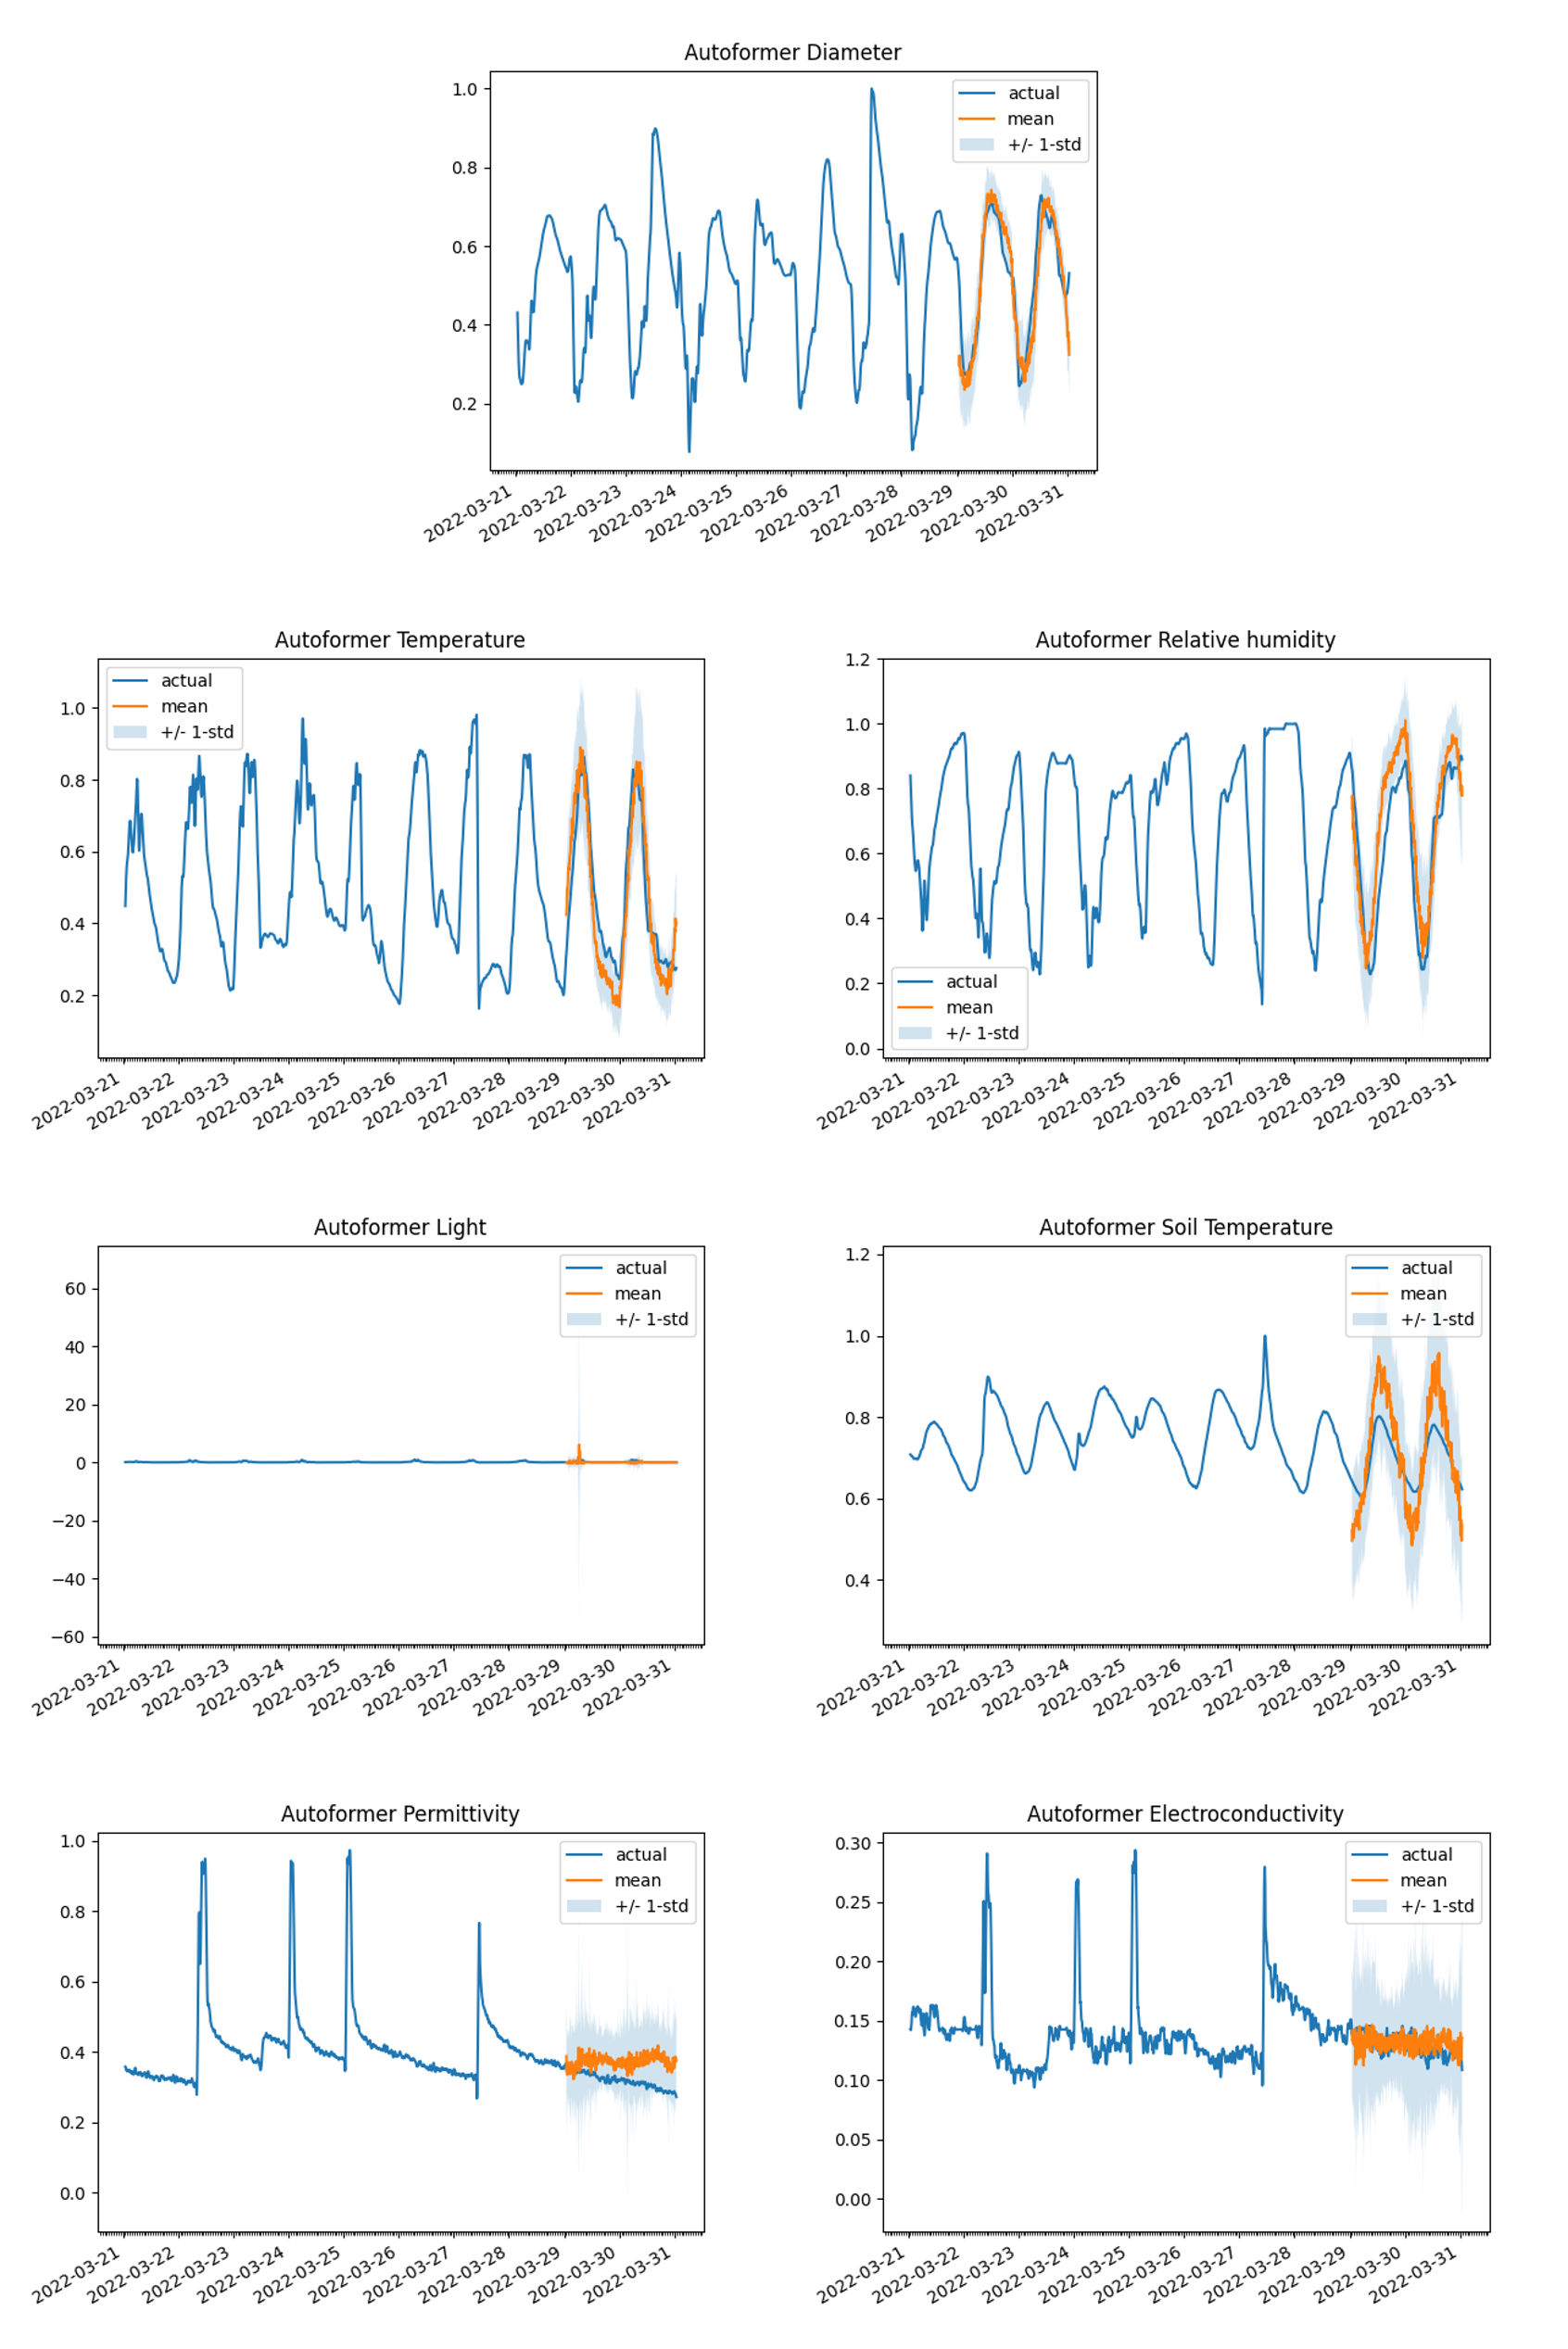
\includegraphics[width=15 cm]{6_ChapterResults/figuras/A11.png}
    \caption{Comparison between the predicted values generated by the A11 model and the actual observed values for the 7 variables over a two-day prediction horizon}
    \label{A11}
\end{figure}

\section{Effect of Dropout}
In this section, we examine the results of experiments that involved varying the Dropout rates across different models. Dropout is a regularization technique used to prevent overfitting by randomly dropping units during training, and its impact on model performance can be significant. By adjusting Dropout rates, we aim to understand how this parameter influences the models' ability to generalize, specifically in terms of their predictive accuracy and stability.

\subsection{Transformer}
The results for the Transformer variant with modified Dropout values, as shown in Tables \ref{T3_M} and \ref{T3_R}, indicate mixed performance compared to the T13 model, which served as the baseline for this experimental phase. While these models underperform in predicting the plant diameter, they show improvement in forecasting the other environmental variables. Due to this enhanced ability to predict a broader range of variables, Model T15 is considered the best model in this phase. Figure \ref{T15} presents a side-by-side comparison of the T15 model's predictions against the actual values, showcasing the model's predictive accuracy.

Additionally, as seen in \ref{T3_T}, adjusting the Dropout values has minimal impact on training times, with little to no variation observed.


\begin{table}[]
    \centering
    \resizebox{\textwidth}{!}{%
    \begin{tabular}{ccccccccc}
    \multicolumn{9}{c}{\textbf{MSE   (Sorted by model)}}                                                                                                                                                                                                                          \\
    Model & Diameter                       & Electroconductivity            & Light                          & Permittivity                   & Relative Humidity              & Soil Temperature               & Temperature                    & Mean                           \\
    T14   & \cellcolor[HTML]{F8696B}-19.46 & \cellcolor[HTML]{F8696B}-23.07 & \cellcolor[HTML]{FFEB84}-14.03 & \cellcolor[HTML]{F8696B}-5.46  & \cellcolor[HTML]{63BE7B}-19.15 & \cellcolor[HTML]{F8696B}-12.16 & \cellcolor[HTML]{63BE7B}-20.31 & \cellcolor[HTML]{F8696B}-16.23 \\
    T15   & \cellcolor[HTML]{63BE7B}-20.48 & \cellcolor[HTML]{FFEB84}-30.30 & \cellcolor[HTML]{63BE7B}-14.25 & \cellcolor[HTML]{63BE7B}-34.57 & \cellcolor[HTML]{FFEB84}-15.44 & \cellcolor[HTML]{63BE7B}-23.28 & \cellcolor[HTML]{FFEB84}-17.85 & \cellcolor[HTML]{63BE7B}-22.31 \\
    T16   & \cellcolor[HTML]{FFEB84}-19.75 & \cellcolor[HTML]{63BE7B}-37.64 & \cellcolor[HTML]{F8696B}-13.06 & \cellcolor[HTML]{FFEB84}-24.54 & \cellcolor[HTML]{F8696B}-8.32  & \cellcolor[HTML]{FFEB84}-12.23 & \cellcolor[HTML]{F8696B}-16.79 & \cellcolor[HTML]{FFEB84}-18.91
    \end{tabular}%
    }
    \caption{Mean Squared Errors (MSE) for different Transformer models obtained by varying the Dropout, sorted by model}
    \label{T3_M}
    \end{table}


\begin{table}[]
    \centering
    \resizebox{\textwidth}{!}{%
    \begin{tabular}{ccccccccc}
    \multicolumn{9}{c}{\textbf{R2 (Sorted by model)}}                                                                                                                                                                                                                       \\
    Model & Diameter                     & Electroconductivity            & Light                        & Permittivity                    & Relative\_humidity            & Soil\_Temperature              & Temperature                  & Mean                           \\
    T14   & \cellcolor[HTML]{F8696B}0.49 & \cellcolor[HTML]{F8696B}-59.79 & \cellcolor[HTML]{FFEB84}0.31 & \cellcolor[HTML]{F8696B}-620.24 & \cellcolor[HTML]{63BE7B}0.76  & \cellcolor[HTML]{F8696B}-15.16 & \cellcolor[HTML]{63BE7B}0.76 & \cellcolor[HTML]{F8696B}-98.98 \\
    T15   & \cellcolor[HTML]{63BE7B}0.60 & \cellcolor[HTML]{FFEB84}-10.51 & \cellcolor[HTML]{63BE7B}0.34 & \cellcolor[HTML]{63BE7B}0.24    & \cellcolor[HTML]{FFEB84}0.44  & \cellcolor[HTML]{63BE7B}-0.25  & \cellcolor[HTML]{FFEB84}0.58 & \cellcolor[HTML]{63BE7B}-1.22  \\
    T16   & \cellcolor[HTML]{FFEB84}0.52 & \cellcolor[HTML]{63BE7B}-1.12  & \cellcolor[HTML]{F8696B}0.14 & \cellcolor[HTML]{FFEB84}-6.68   & \cellcolor[HTML]{F8696B}-1.91 & \cellcolor[HTML]{FFEB84}-14.90 & \cellcolor[HTML]{F8696B}0.47 & \cellcolor[HTML]{FFEB84}-3.36 
    \end{tabular}%
    }
    \caption{R-squared (R²) for different Transformer models obtained by varying the Dropout, sorted by model}
    \label{T3_R}
    \end{table}



\begin{table}[]
    \begin{tabular}{cc}
    \multicolumn{2}{c}{\textbf{Training   Time (Sorted by model)}} \\
    Model             & Training time {[}s{]}                      \\
    T14               & \cellcolor[HTML]{63BE7B}252.21             \\
    T15               & \cellcolor[HTML]{FFEB84}257.21             \\
    T16               & \cellcolor[HTML]{F8696B}258.09            
    \end{tabular}
    \caption{Training times for different Transformer models obtained by varying the Dropout, sorted by model}
    \label{T3_T}
    \end{table}

\begin{figure}[htbp]
    \centering
    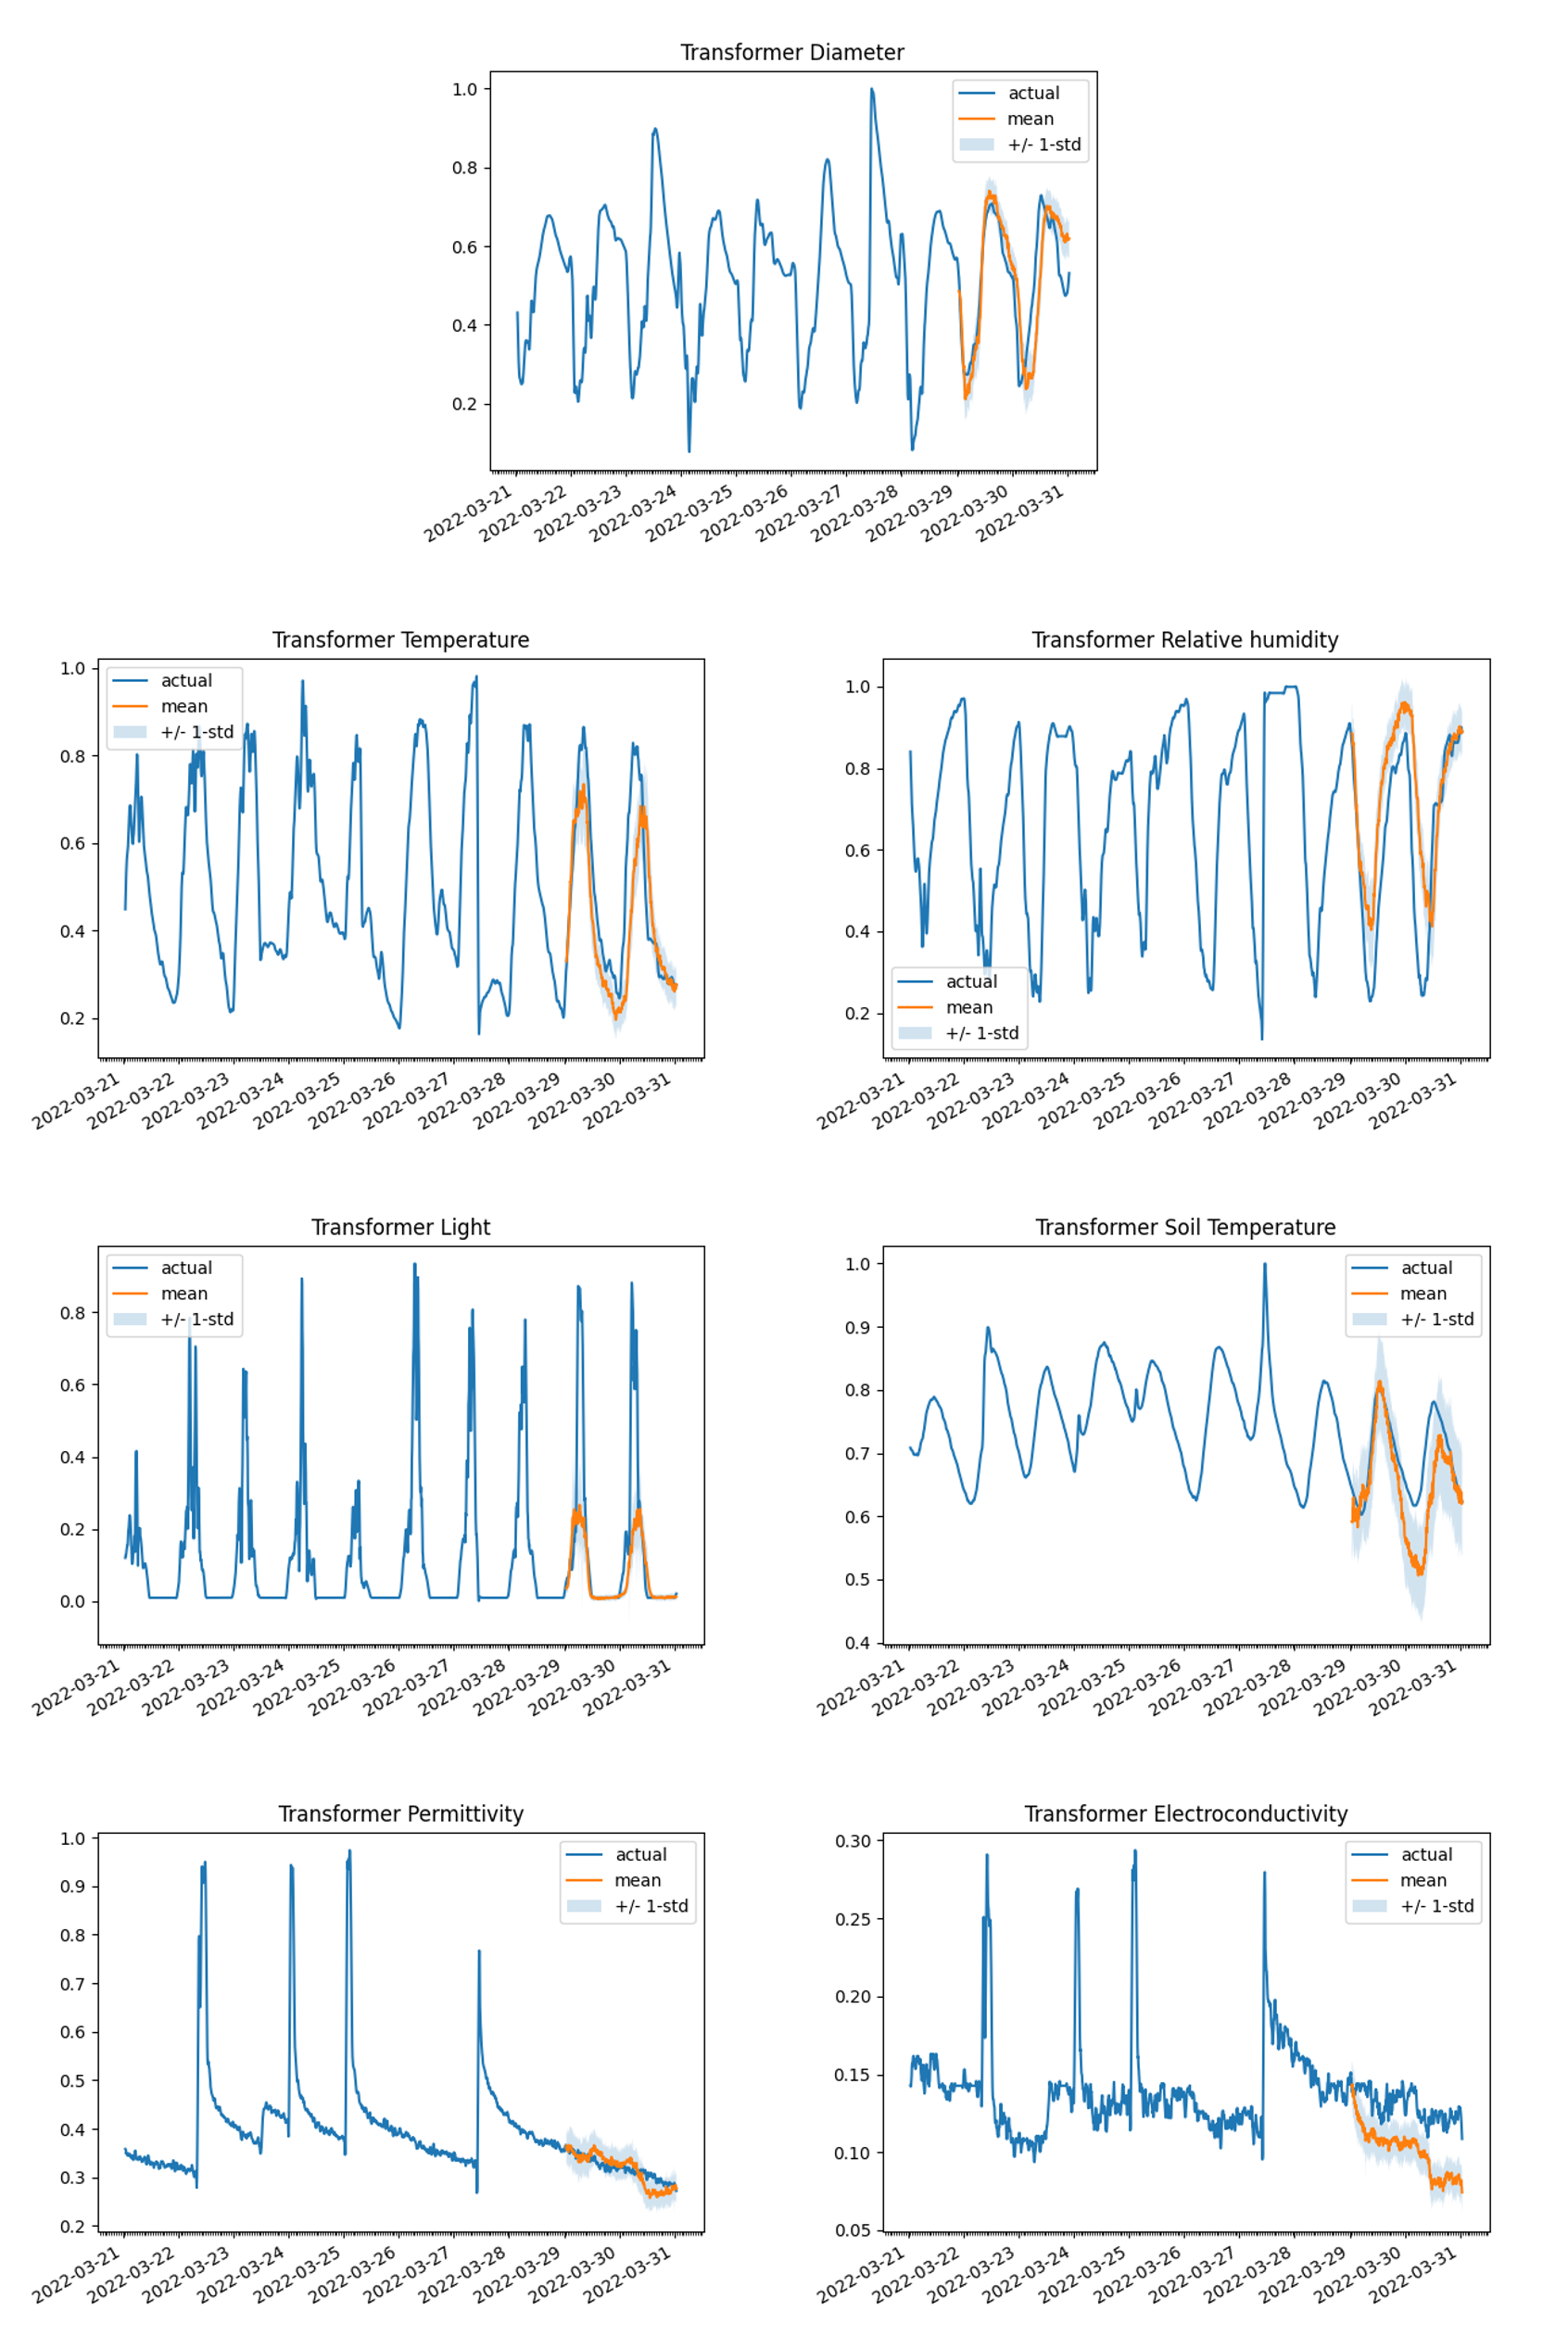
\includegraphics[width=15 cm]{6_ChapterResults/figuras/T15.png}
    \caption{Comparison between the predicted values generated by the T15 model and the actual observed values for the 7 variables over a two-day prediction horizon}
    \label{T15}
\end{figure}

\subsection{Informer}
The results for the Informer variant with modified Dropout values, as shown in Tables \ref{I3_M} and \ref{I3_R}, reveal slight improvements in predicting plant diameter compared to the I13 model, which served as the baseline for this experimental phase. However, these models perform slightly worse when predicting other environmental variables. As a result, I13 remains the best model obtained so far.

Additionally, as seen in Table \ref{I3_T}, training times increase slightly with changes in Dropout values, but the impact on computational efficiency is minimal.


\begin{table}[]
    \centering
    \resizebox{\textwidth}{!}{%
    \begin{tabular}{ccccccccc}
    \multicolumn{9}{c}{\textbf{MSE   (Sorted by model)}}                                                                                                                                                                                                                          \\
    Model & Diameter                       & Electroconductivity            & Light                          & Permittivity                   & Relative\_humidity             & Soil\_Temperature              & Temperature                    & Mean                           \\
    I14   & \cellcolor[HTML]{F8696B}-18.29 & \cellcolor[HTML]{FFEB84}-28.35 & \cellcolor[HTML]{F8696B}-12.21 & \cellcolor[HTML]{F8696B}-24.76 & \cellcolor[HTML]{63BE7B}-11.89 & \cellcolor[HTML]{FFEB84}-9.29  & \cellcolor[HTML]{FFEB84}-13.23 & \cellcolor[HTML]{F8696B}-16.86 \\
    I15   & \cellcolor[HTML]{FFEB84}-22.29 & \cellcolor[HTML]{63BE7B}-33.13 & \cellcolor[HTML]{FFEB84}-12.63 & \cellcolor[HTML]{63BE7B}-29.98 & \cellcolor[HTML]{FFEB84}-11.37 & \cellcolor[HTML]{F8696B}-8.38  & \cellcolor[HTML]{F8696B}-11.97 & \cellcolor[HTML]{63BE7B}-18.54 \\
    I16   & \cellcolor[HTML]{63BE7B}-22.99 & \cellcolor[HTML]{F8696B}-25.84 & \cellcolor[HTML]{63BE7B}-12.76 & \cellcolor[HTML]{FFEB84}-24.76 & \cellcolor[HTML]{F8696B}-9.70  & \cellcolor[HTML]{63BE7B}-10.53 & \cellcolor[HTML]{63BE7B}-13.48 & \cellcolor[HTML]{FFEB84}-17.15
    \end{tabular}%
    }
    \caption{Mean Squared Errors (MSE) for different Informer models obtained by varying the Dropout, sorted by model}
    \label{I3_M}
    \end{table}

\begin{table}[]
    \centering
    \resizebox{\textwidth}{!}{%
    \begin{tabular}{ccccccccc}
    \multicolumn{9}{c}{\textbf{R2 (Sorted by model)}}                                                                                                                                                                                                                      \\
    Model & Diameter                     & Electroconductivity            & Light                         & Permittivity                  & Relative\_humidity            & Soil\_Temperature              & Temperature                   & Mean                          \\
    I14   & \cellcolor[HTML]{F8696B}0.33 & \cellcolor[HTML]{FFEB84}-17.00 & \cellcolor[HTML]{F8696B}-0.05 & \cellcolor[HTML]{F8696B}-6.30 & \cellcolor[HTML]{63BE7B}-0.28 & \cellcolor[HTML]{FFEB84}-30.30 & \cellcolor[HTML]{FFEB84}-0.21 & \cellcolor[HTML]{FFEB84}-7.69 \\
    I15   & \cellcolor[HTML]{FFEB84}0.73 & \cellcolor[HTML]{63BE7B}-4.99  & \cellcolor[HTML]{FFEB84}0.05  & \cellcolor[HTML]{63BE7B}-1.19 & \cellcolor[HTML]{FFEB84}-0.44 & \cellcolor[HTML]{F8696B}-37.60 & \cellcolor[HTML]{F8696B}-0.62 & \cellcolor[HTML]{63BE7B}-6.29 \\
    I16   & \cellcolor[HTML]{63BE7B}0.77 & \cellcolor[HTML]{F8696B}-31.09 & \cellcolor[HTML]{63BE7B}0.07  & \cellcolor[HTML]{FFEB84}-6.30 & \cellcolor[HTML]{F8696B}-1.12 & \cellcolor[HTML]{63BE7B}-22.52 & \cellcolor[HTML]{63BE7B}-0.14 & \cellcolor[HTML]{F8696B}-8.62
    \end{tabular}%
    }
    \caption{R-squared (R²) for different Informer models obtained by varying the Dropout, sorted by model}
    \label{I3_R}
    \end{table}


\begin{table}[]
    \begin{tabular}{cc}
    \multicolumn{2}{c}{\textbf{Training   Time (Sorted by model)}} \\
    Model             & Training time {[}s{]}                      \\
    I14               & \cellcolor[HTML]{63BE7B}140.69             \\
    I15               & \cellcolor[HTML]{FFEB84}142.24             \\
    I16               & \cellcolor[HTML]{F8696B}145.03            
    \end{tabular}
    \caption{Training times for different Informer models obtained by varying the Dropout, sorted by model}
    \label{I3_T}
    \end{table}


\subsection{Autoformer}
The results for the Autoformer variant with modified Dropout values, as shown in Tables \ref{A3_M} and \ref{A3_R}, indicate varied outcomes compared to the A11 model, which served as the baseline for this experimental phase. While specific details about performance changes are not provided, the variations in Dropout likely influenced the model's ability to generalize and prevent overfitting.

Additionally, as seen in Table \ref{A3_T}, training times were reduced when Dropout was applied. This reduction in training time suggests that the model may have been more efficient during training, likely due to the regularization effect of Dropout, which reduces the complexity of the model during the learning process.


\begin{table}[]
    \centering
    \resizebox{\textwidth}{!}{%
    \begin{tabular}{ccccccccc}
    \multicolumn{9}{c}{\textbf{MSE   (Sorted by model)}}                                                                                                                                                                                                                          \\
    Model & Diameter                       & Electroconductivity            & Light                          & Permittivity                   & Relative\_humidity             & Soil\_Temperature              & Temperature                    & Mean                           \\
    A14   & \cellcolor[HTML]{63BE7B}-25.21 & \cellcolor[HTML]{F8696B}-37.91 & \cellcolor[HTML]{FFEB84}-11.47 & \cellcolor[HTML]{F8696B}-23.76 & \cellcolor[HTML]{63BE7B}-20.63 & \cellcolor[HTML]{63BE7B}-18.92 & \cellcolor[HTML]{63BE7B}-23.66 & \cellcolor[HTML]{63BE7B}-23.08 \\
    A15   & \cellcolor[HTML]{FFEB84}-20.46 & \cellcolor[HTML]{FFEB84}-38.95 & \cellcolor[HTML]{63BE7B}-11.67 & \cellcolor[HTML]{FFEB84}-24.51 & \cellcolor[HTML]{FFEB84}-15.36 & \cellcolor[HTML]{F8696B}-16.75 & \cellcolor[HTML]{FFEB84}-20.50 & \cellcolor[HTML]{FFEB84}-21.17 \\
    A16   & \cellcolor[HTML]{F8696B}-18.64 & \cellcolor[HTML]{63BE7B}-39.43 & \cellcolor[HTML]{F8696B}-11.18 & \cellcolor[HTML]{63BE7B}-27.39 & \cellcolor[HTML]{F8696B}-14.12 & \cellcolor[HTML]{FFEB84}-18.22 & \cellcolor[HTML]{F8696B}-16.85 & \cellcolor[HTML]{F8696B}-20.83
    \end{tabular}%
    }
    \caption{Mean Squared Errors (MSE) for different Autoformer models obtained by varying the Dropout, sorted by model}
    \label{A3_M}
    \end{table}


\begin{table}[]
    \centering
    \resizebox{\textwidth}{!}{%
    \begin{tabular}{ccccccccc}
    \multicolumn{9}{c}{\textbf{R2 (Sorted by model)}}                                                                                                                                                                                                                  \\
    Model & Diameter                     & Electroconductivity           & Light                         & Permittivity                  & Relative\_humidity           & Soil\_Temperature             & Temperature                  & Mean                          \\
    A14   & \cellcolor[HTML]{63BE7B}0.86 & \cellcolor[HTML]{F8696B}-0.99 & \cellcolor[HTML]{FFEB84}-0.25 & \cellcolor[HTML]{F8696B}-8.20 & \cellcolor[HTML]{63BE7B}0.83 & \cellcolor[HTML]{63BE7B}-2.41 & \cellcolor[HTML]{63BE7B}0.89 & \cellcolor[HTML]{FFEB84}-1.32 \\
    A15   & \cellcolor[HTML]{FFEB84}0.59 & \cellcolor[HTML]{FFEB84}-0.57 & \cellcolor[HTML]{63BE7B}-0.19 & \cellcolor[HTML]{FFEB84}-6.72 & \cellcolor[HTML]{FFEB84}0.42 & \cellcolor[HTML]{F8696B}-4.62 & \cellcolor[HTML]{FFEB84}0.77 & \cellcolor[HTML]{F8696B}-1.47 \\
    A16   & \cellcolor[HTML]{F8696B}0.38 & \cellcolor[HTML]{63BE7B}-0.41 & \cellcolor[HTML]{F8696B}-0.33 & \cellcolor[HTML]{63BE7B}-2.98 & \cellcolor[HTML]{F8696B}0.24 & \cellcolor[HTML]{FFEB84}-3.00 & \cellcolor[HTML]{F8696B}0.47 & \cellcolor[HTML]{63BE7B}-0.80
    \end{tabular}%
    }
    \caption{R-squared (R²) for different Autoformer models obtained by varying the Dropout, sorted by model}
    \label{A3_R}
    \end{table}


\begin{table}[]
    \begin{tabular}{cc}
    \multicolumn{2}{c}{\textbf{Training   Time (Sorted by model)}} \\
    Model             & Training time {[}s{]}                      \\
    A14               & \cellcolor[HTML]{F8696B}308.12             \\
    A15               & \cellcolor[HTML]{FFEB84}304.43             \\
    A16               & \cellcolor[HTML]{63BE7B}298.24            
    \end{tabular}
    \caption{Training times for different Autoformer models obtained by varying the Dropout, sorted by model}
    \label{A3_T}
    \end{table}

\section{Effect of Encoder Layers, Decoder Layers, and Dimensionality of the Transformer Layers}

In this section, we present the results of experiments involving changes to the Encoder Layers, Decoder Layers, and Dimensionality of the Transformer Layers across various model variants. This phase of experimentation aims to explore how modifications in these architectural parameters impact the performance of the Transformer, Informer, and Autoformer models. By systematically adjusting these key aspects of the model architecture, we seek to identify configurations that optimize predictive accuracy while balancing computational efficiency.

\subsection{Transformer}
The results for the Transformer variant with modified Encoder Layers, Decoder Layers, and Dimensionality, as shown in Tables \ref{T4_M} and \ref{T4_R}, exhibit mixed performance compared to the T15 model, which served as the baseline for this phase of experimentation. Some models showed better results in specific variables, while others performed worse. These variations can be attributed to changes in model complexity. On one hand, adding layers or increasing dimensionality can enhance the model's ability to capture complex patterns; on the other hand, it can also lead to overfitting or increased difficulty in effective training. However, none of these models significantly outperformed the existing ones, and as a result, T15 remains the best model among those tested.

Additionally, as seen in Table \ref{T4_T}, increasing the number of layers leads to higher computational costs and, consequently, longer training times.


\begin{table}[]
    \centering
    \resizebox{\textwidth}{!}{%
    \begin{tabular}{ccccccccc}
    \multicolumn{9}{c}{\textbf{MSE   (Sorted by model)}}                                                                                                                                                                                                                          \\
    Model & Diameter                       & Electroconductivity            & Light                          & Permittivity                   & Relative Humidity              & Soil Temperature               & Temperature                    & Mean                           \\
    T17   & \cellcolor[HTML]{FDB47A}-18.99 & \cellcolor[HTML]{A7D17E}-36.81 & \cellcolor[HTML]{F8696B}-12.59 & \cellcolor[HTML]{7AC47C}-27.62 & \cellcolor[HTML]{FA8E72}-10.95 & \cellcolor[HTML]{FFE182}-12.36 & \cellcolor[HTML]{FB9073}-15.53 & \cellcolor[HTML]{F0E683}-19.26 \\
    T18   & \cellcolor[HTML]{CDDC81}-21.58 & \cellcolor[HTML]{F8696B}-19.96 & \cellcolor[HTML]{FED280}-13.93 & \cellcolor[HTML]{F8696B}-9.39  & \cellcolor[HTML]{F8696B}-10.04 & \cellcolor[HTML]{F8696B}-8.74  & \cellcolor[HTML]{F0E683}-18.71 & \cellcolor[HTML]{F8696B}-14.62 \\
    T19   & \cellcolor[HTML]{E6E382}-20.99 & \cellcolor[HTML]{63BE7B}-43.19 & \cellcolor[HTML]{D9E081}-14.58 & \cellcolor[HTML]{C2D980}-23.41 & \cellcolor[HTML]{FAE983}-13.54 & \cellcolor[HTML]{9CCE7E}-21.04 & \cellcolor[HTML]{D9E081}-19.58 & \cellcolor[HTML]{63BE7B}-22.33 \\
    T20   & \cellcolor[HTML]{F8696B}-17.07 & \cellcolor[HTML]{DBE081}-31.96 & \cellcolor[HTML]{FCAC78}-13.45 & \cellcolor[HTML]{FFDC81}-18.60 & \cellcolor[HTML]{FFE283}-13.08 & \cellcolor[HTML]{FBE983}-13.01 & \cellcolor[HTML]{F8696B}-14.41 & \cellcolor[HTML]{FDBC7B}-17.37 \\
    T21   & \cellcolor[HTML]{63BE7B}-24.14 & \cellcolor[HTML]{FCA577}-23.93 & \cellcolor[HTML]{63BE7B}-15.60 & \cellcolor[HTML]{E9E482}-21.13 & \cellcolor[HTML]{63BE7B}-21.40 & \cellcolor[HTML]{FECF7F}-11.83 & \cellcolor[HTML]{63BE7B}-23.90 & \cellcolor[HTML]{C1D980}-20.28 \\
    T22   & \cellcolor[HTML]{FDEA83}-20.43 & \cellcolor[HTML]{91CB7D}-38.85 & \cellcolor[HTML]{FB9574}-13.14 & \cellcolor[HTML]{63BE7B}-29.00 & \cellcolor[HTML]{FDB87B}-12.01 & \cellcolor[HTML]{89C97D}-22.70 & \cellcolor[HTML]{EFE683}-18.75 & \cellcolor[HTML]{6CC07B}-22.13 \\
    T23   & \cellcolor[HTML]{FFDD82}-20.03 & \cellcolor[HTML]{FDB97B}-25.21 & \cellcolor[HTML]{D6DF81}-14.61 & \cellcolor[HTML]{FB9674}-12.95 & \cellcolor[HTML]{8CC97D}-19.25 & \cellcolor[HTML]{FA8671}-9.61  & \cellcolor[HTML]{FCAA78}-16.29 & \cellcolor[HTML]{FCAC78}-16.85 \\
    T24   & \cellcolor[HTML]{FFEA84}-20.38 & \cellcolor[HTML]{FB9C75}-23.34 & \cellcolor[HTML]{C7DB80}-14.73 & \cellcolor[HTML]{FCA978}-14.51 & \cellcolor[HTML]{F5E883}-13.79 & \cellcolor[HTML]{63BE7B}-25.97 & \cellcolor[HTML]{FFDA81}-17.68 & \cellcolor[HTML]{FFE283}-18.63
    \end{tabular}%
    }
    \caption{Mean Squared Errors (MSE) for different Transformer models obtained by varying the number of Encoder Layers, Decoder Layers, and Dimensionality of the Transformer Layers, sorted by model}
    \label{T4_M}
    \end{table}

\begin{table}[]
    \centering
    \resizebox{\textwidth}{!}{%
    \begin{tabular}{ccccccccc}
    \multicolumn{9}{c}{\textbf{R2 (Sorted by model)}}                                                                                                                                                                                                                        \\
    Model & Diameter                     & Electroconductivity             & Light                        & Permittivity                    & Relative\_humidity            & Soil\_Temperature              & Temperature                  & Mean                           \\
    T17   & \cellcolor[HTML]{FCBF7B}0.43 & \cellcolor[HTML]{72C37C}-1.57   & \cellcolor[HTML]{F8696B}0.04 & \cellcolor[HTML]{6BC17C}-2.77   & \cellcolor[HTML]{FA9773}-0.59 & \cellcolor[HTML]{FEE482}-14.46 & \cellcolor[HTML]{FA9C74}0.29 & \cellcolor[HTML]{8FCB7E}-2.66  \\
    T18   & \cellcolor[HTML]{BFD981}0.69 & \cellcolor[HTML]{F8696B}-123.50 & \cellcolor[HTML]{FDD680}0.29 & \cellcolor[HTML]{F8696B}-250.10 & \cellcolor[HTML]{F8696B}-0.96 & \cellcolor[HTML]{F8696B}-34.52 & \cellcolor[HTML]{E6E483}0.66 & \cellcolor[HTML]{F8696B}-58.21 \\
    T19   & \cellcolor[HTML]{DEE283}0.64 & \cellcolor[HTML]{63BE7B}0.41    & \cellcolor[HTML]{D5DF82}0.39 & \cellcolor[HTML]{9ACE7F}-8.95   & \cellcolor[HTML]{F6E984}0.12  & \cellcolor[HTML]{74C37C}-1.09  & \cellcolor[HTML]{C4DA81}0.72 & \cellcolor[HTML]{73C37C}-1.11  \\
    T20   & \cellcolor[HTML]{F8696B}0.12 & \cellcolor[HTML]{97CD7E}-6.85   & \cellcolor[HTML]{FBB279}0.21 & \cellcolor[HTML]{FEE783}-29.17  & \cellcolor[HTML]{FEE482}0.03  & \cellcolor[HTML]{F3E884}-12.29 & \cellcolor[HTML]{F8696B}0.08 & \cellcolor[HTML]{D9E082}-6.84  \\
    T21   & \cellcolor[HTML]{63BE7B}0.83 & \cellcolor[HTML]{FDC87D}-48.88  & \cellcolor[HTML]{63BE7B}0.52 & \cellcolor[HTML]{CDDD82}-15.83  & \cellcolor[HTML]{63BE7B}0.86  & \cellcolor[HTML]{FDD880}-16.43 & \cellcolor[HTML]{63BE7B}0.90 & \cellcolor[HTML]{FEE582}-11.15 \\
    T22   & \cellcolor[HTML]{FEEB84}0.59 & \cellcolor[HTML]{6BC17C}-0.61   & \cellcolor[HTML]{FA9A74}0.15 & \cellcolor[HTML]{63BE7B}-1.75   & \cellcolor[HTML]{FCC27C}-0.24 & \cellcolor[HTML]{6CC17C}-0.43  & \cellcolor[HTML]{E5E483}0.66 & \cellcolor[HTML]{63BE7B}-0.23  \\
    T23   & \cellcolor[HTML]{FEE082}0.55 & \cellcolor[HTML]{FDD880}-36.09  & \cellcolor[HTML]{D1DE82}0.40 & \cellcolor[HTML]{FCB97A}-109.74 & \cellcolor[HTML]{76C47D}0.77  & \cellcolor[HTML]{FA9072}-28.06 & \cellcolor[HTML]{FCB77A}0.40 & \cellcolor[HTML]{FCC17C}-24.54 \\
    T24   & \cellcolor[HTML]{FEEA83}0.59 & \cellcolor[HTML]{FCBE7B}-56.16  & \cellcolor[HTML]{C2DA81}0.41 & \cellcolor[HTML]{FDCC7E}-76.37  & \cellcolor[HTML]{ECE683}0.17  & \cellcolor[HTML]{63BE7B}0.33   & \cellcolor[HTML]{FEDF81}0.56 & \cellcolor[HTML]{FDD17F}-18.64
    \end{tabular}%
    }
    \caption{R-squared (R²) for different Transformer models obtained by varying the number of Encoder Layers, Decoder Layers, and Dimensionality of the Transformer Layers, sorted by model}
    \label{T4_R}
    \end{table}



\begin{table}[]
    \begin{tabular}{ccccc}
    \multicolumn{2}{c}{\textbf{Training   Time (Sorted by model)}} &  & \multicolumn{2}{c}{\textbf{Training Time (Sorted   by model)}} \\
    Model             & Training time {[}s{]}                      &  & Model             & Training time {[}s{]}                      \\
    T17               & \cellcolor[HTML]{63BE7B}143.56             &  & T17               & \cellcolor[HTML]{63BE7B}143.56             \\
    T18               & \cellcolor[HTML]{A8D17E}197.91             &  & T18               & \cellcolor[HTML]{A8D17E}197.91             \\
    T19               & \cellcolor[HTML]{FFE483}275.11             &  & T20               & \cellcolor[HTML]{A8D17E}198.02             \\
    T20               & \cellcolor[HTML]{A8D17E}198.02             &  & T22               & \cellcolor[HTML]{F3E783}257.47             \\
    T21               & \cellcolor[HTML]{FBA176}351.72             &  & T19               & \cellcolor[HTML]{FFE483}275.11             \\
    T22               & \cellcolor[HTML]{F3E783}257.47             &  & T23               & \cellcolor[HTML]{FDC17C}315.29             \\
    T23               & \cellcolor[HTML]{FDC17C}315.29             &  & T21               & \cellcolor[HTML]{FBA176}351.72             \\
    T24               & \cellcolor[HTML]{F8696B}415.78             &  & T24               & \cellcolor[HTML]{F8696B}415.78            
    \end{tabular}
    \caption{Training times for different Transformer models obtained by varying the number of Encoder Layers, Decoder Layers, and Dimensionality of the Transformer Layers, sorted by model and training time values}
    \label{T4_T}
    \end{table}


\subsection{Informer}
The results for the Informer variant with modified Encoder Layers, Decoder Layers, and Dimensionality of the Transformer Layers, as shown in Tables \ref{I4_M} and \ref{I4_R}, reveal a range of performance outcomes when compared to the I13 model, which was used as the baseline for this experimental phase. Similar to the Transformer results, the performance across these models is quite varied. Among all the models tested, I20 is considered the best due to its superior overall performance. The effectiveness of the I20 model is demonstrated in Figure \ref{I20}, where its predictions are compared with the corresponding real values.

Additionally, as seen in Table \ref{I4_T}, increasing the number of layers results in higher computational costs, just as with the Transformer models. However, when compared to the Transformer models, the Informer models remain more computationally efficient despite the increased complexity.




\begin{table}[]
    \centering
    \resizebox{\textwidth}{!}{%
    \begin{tabular}{ccccccccc}
    \multicolumn{9}{c}{\textbf{MSE   (Sorted by model)}}                                                                                                                                                                                                                          \\
    Model & Diameter                       & Electroconductivity            & Light                          & Permittivity                   & Relative\_humidity             & Soil\_Temperature              & Temperature                    & Mean                           \\
    I17   & \cellcolor[HTML]{97CD7E}-21.74 & \cellcolor[HTML]{DEE182}-29.26 & \cellcolor[HTML]{63BE7B}-13.13 & \cellcolor[HTML]{E1E282}-16.98 & \cellcolor[HTML]{63BE7B}-11.97 & \cellcolor[HTML]{E0E282}-17.31 & \cellcolor[HTML]{A7D17E}-15.57 & \cellcolor[HTML]{9FCF7E}-18.00 \\
    I18   & \cellcolor[HTML]{FFDB81}-19.94 & \cellcolor[HTML]{63BE7B}-34.20 & \cellcolor[HTML]{C9DB80}-12.68 & \cellcolor[HTML]{63BE7B}-28.54 & \cellcolor[HTML]{FFDD82}-11.06 & \cellcolor[HTML]{FCAF79}-13.65 & \cellcolor[HTML]{F9E983}-13.84 & \cellcolor[HTML]{63BE7B}-19.13 \\
    I19   & \cellcolor[HTML]{FDB97B}-18.59 & \cellcolor[HTML]{F97C6F}-23.47 & \cellcolor[HTML]{FB9F76}-11.87 & \cellcolor[HTML]{FECB7E}-13.04 & \cellcolor[HTML]{E6E382}-11.42 & \cellcolor[HTML]{D1DD81}-17.94 & \cellcolor[HTML]{FFE683}-13.60 & \cellcolor[HTML]{FDBF7C}-15.70 \\
    I20   & \cellcolor[HTML]{C0D980}-21.30 & \cellcolor[HTML]{F8696B}-22.74 & \cellcolor[HTML]{CEDD81}-12.65 & \cellcolor[HTML]{F8696B}-9.33  & \cellcolor[HTML]{D7DF81}-11.48 & \cellcolor[HTML]{C1D980}-18.62 & \cellcolor[HTML]{63BE7B}-17.01 & \cellcolor[HTML]{FFE784}-16.16 \\
    I21   & \cellcolor[HTML]{FB9F76}-17.53 & \cellcolor[HTML]{F2E783}-28.47 & \cellcolor[HTML]{F8696B}-11.46 & \cellcolor[HTML]{FA8A72}-10.58 & \cellcolor[HTML]{FFE583}-11.21 & \cellcolor[HTML]{FA8972}-12.19 & \cellcolor[HTML]{FA7F70}-11.48 & \cellcolor[HTML]{F8696B}-14.70 \\
    I22   & \cellcolor[HTML]{63BE7B}-22.32 & \cellcolor[HTML]{F9706D}-22.99 & \cellcolor[HTML]{FFDF82}-12.35 & \cellcolor[HTML]{FDBD7C}-12.49 & \cellcolor[HTML]{B7D67F}-11.61 & \cellcolor[HTML]{63BE7B}-22.68 & \cellcolor[HTML]{A4D07E}-15.63 & \cellcolor[HTML]{CCDC81}-17.15 \\
    I23   & \cellcolor[HTML]{A1D07E}-21.63 & \cellcolor[HTML]{FFDF82}-27.44 & \cellcolor[HTML]{EAE582}-12.53 & \cellcolor[HTML]{C8DB80}-19.23 & \cellcolor[HTML]{FFDE82}-11.09 & \cellcolor[HTML]{F8696B}-10.97 & \cellcolor[HTML]{F8696B}-11.03 & \cellcolor[HTML]{FBEA83}-16.28 \\
    I24   & \cellcolor[HTML]{F8696B}-15.39 & \cellcolor[HTML]{B6D67F}-30.86 & \cellcolor[HTML]{F9786E}-11.58 & \cellcolor[HTML]{F1E783}-15.46 & \cellcolor[HTML]{F8696B}-9.11  & \cellcolor[HTML]{FEC97E}-14.66 & \cellcolor[HTML]{F9736D}-11.22 & \cellcolor[HTML]{FCAB78}-15.47
    \end{tabular}%
    }
    \caption{Mean Squared Errors (MSE) for different Informer models obtained by varying the number of Encoder Layers, Decoder Layers, and Dimensionality of the Transformer Layers, sorted by model}
    \label{I4_M}
    \end{table}


    


\begin{table}[]
    \centering
    \resizebox{\textwidth}{!}{%
    \begin{tabular}{ccccccccc}
    \multicolumn{9}{c}{\textbf{R2 (Sorted by model)}}                                                                                                                                                                                                                          \\
    Model & Diameter                      & Electroconductivity            & Light                         & Permittivity                    & Relative\_humidity            & Soil\_Temperature              & Temperature                   & Mean                           \\
    I17   & \cellcolor[HTML]{90CB7E}0.70  & \cellcolor[HTML]{CADC81}-13.62 & \cellcolor[HTML]{63BE7B}0.15  & \cellcolor[HTML]{B1D580}-42.75  & \cellcolor[HTML]{63BE7B}-0.26 & \cellcolor[HTML]{C5DB81}-3.94  & \cellcolor[HTML]{99CE7F}0.29  & \cellcolor[HTML]{A2D17F}-8.49  \\
    I18   & \cellcolor[HTML]{FEE282}0.54  & \cellcolor[HTML]{63BE7B}-3.68  & \cellcolor[HTML]{C7DB81}0.06  & \cellcolor[HTML]{63BE7B}-2.05   & \cellcolor[HTML]{FEDF81}-0.55 & \cellcolor[HTML]{FCC27C}-10.47 & \cellcolor[HTML]{F8E984}-0.06 & \cellcolor[HTML]{63BE7B}-2.32  \\
    I19   & \cellcolor[HTML]{FDCA7D}0.38  & \cellcolor[HTML]{F98570}-54.40 & \cellcolor[HTML]{FBA276}-0.14 & \cellcolor[HTML]{FED980}-107.44 & \cellcolor[HTML]{E5E483}-0.43 & \cellcolor[HTML]{B3D580}-3.27  & \cellcolor[HTML]{FEE683}-0.11 & \cellcolor[HTML]{FDCF7E}-23.63 \\
    I20   & \cellcolor[HTML]{B7D780}0.67  & \cellcolor[HTML]{F8696B}-64.56 & \cellcolor[HTML]{CCDD82}0.05  & \cellcolor[HTML]{F8696B}-253.73 & \cellcolor[HTML]{D5DF82}-0.41 & \cellcolor[HTML]{A2D07F}-2.65  & \cellcolor[HTML]{63BE7B}0.49  & \cellcolor[HTML]{F8696B}-45.73 \\
    I21   & \cellcolor[HTML]{FBB178}0.20  & \cellcolor[HTML]{E8E583}-16.54 & \cellcolor[HTML]{F8696B}-0.25 & \cellcolor[HTML]{FA9974}-190.27 & \cellcolor[HTML]{FEE683}-0.50 & \cellcolor[HTML]{FA9874}-15.06 & \cellcolor[HTML]{F98470}-0.82 & \cellcolor[HTML]{FBA877}-31.89 \\
    I22   & \cellcolor[HTML]{63BE7B}0.74  & \cellcolor[HTML]{F8736C}-60.91 & \cellcolor[HTML]{FEE081}-0.02 & \cellcolor[HTML]{FDCE7E}-121.98 & \cellcolor[HTML]{B5D680}-0.36 & \cellcolor[HTML]{63BE7B}-0.43  & \cellcolor[HTML]{97CD7E}0.30  & \cellcolor[HTML]{FCC37C}-26.09 \\
    I23   & \cellcolor[HTML]{9ACE7F}0.69  & \cellcolor[HTML]{FEE482}-21.21 & \cellcolor[HTML]{E9E583}0.03  & \cellcolor[HTML]{8FCB7E}-25.07  & \cellcolor[HTML]{FEE082}-0.54 & \cellcolor[HTML]{F8696B}-20.26 & \cellcolor[HTML]{F8696B}-1.01 & \cellcolor[HTML]{AED480}-9.63  \\
    I24   & \cellcolor[HTML]{F8696B}-0.31 & \cellcolor[HTML]{9BCF7F}-9.11  & \cellcolor[HTML]{F8796E}-0.22 & \cellcolor[HTML]{D3DF82}-61.05  & \cellcolor[HTML]{F8696B}-1.43 & \cellcolor[HTML]{FDD880}-8.09  & \cellcolor[HTML]{F8756D}-0.93 & \cellcolor[HTML]{C2DA81}-11.59
    \end{tabular}%
    }
    \caption{R-squared (R²) for different Informer models obtained by varying the number of Encoder Layers, Decoder Layers, and Dimensionality of the Transformer Layers, sorted by model}
    \label{I4_R}
    \end{table}



    

\begin{table}[]
    \begin{tabular}{ccccc}
    \multicolumn{2}{c}{\textbf{Training   Time (Sorted by model)}} &  & \multicolumn{2}{c}{\textbf{Training Time (Sorted   by training time)}} \\
    Model             & Training time {[}s{]}                      &  & Model                 & Training time {[}s{]}                          \\
    I17               & \cellcolor[HTML]{63BE7B}102.57             &  & I17                   & \cellcolor[HTML]{63BE7B}102.57                 \\
    I18               & \cellcolor[HTML]{E1E282}138.04             &  & I20                   & \cellcolor[HTML]{A9D27F}122.21                 \\
    I19               & \cellcolor[HTML]{F9776E}191.89             &  & I22                   & \cellcolor[HTML]{C0D980}128.8                  \\
    I20               & \cellcolor[HTML]{A9D27F}122.21             &  & I18                   & \cellcolor[HTML]{E1E282}138.04                 \\
    I21               & \cellcolor[HTML]{FA7D6F}189.34             &  & I23                   & \cellcolor[HTML]{FED781}154.3                  \\
    I22               & \cellcolor[HTML]{C0D980}128.8              &  & I21                   & \cellcolor[HTML]{FA7D6F}189.34                 \\
    I23               & \cellcolor[HTML]{FED781}154.3              &  & I19                   & \cellcolor[HTML]{F9776E}191.89                 \\
    I24               & \cellcolor[HTML]{F8696B}196.99             &  & I24                   & \cellcolor[HTML]{F8696B}196.99                
    \end{tabular}
    \caption{Training times for different Informer models obtained by varying the number of Encoder Layers, Decoder Layers, and Dimensionality of the Transformer Layers, sorted by model and training time values}
    \label{I4_T}
    \end{table}

\begin{figure}[htbp]
    \centering
    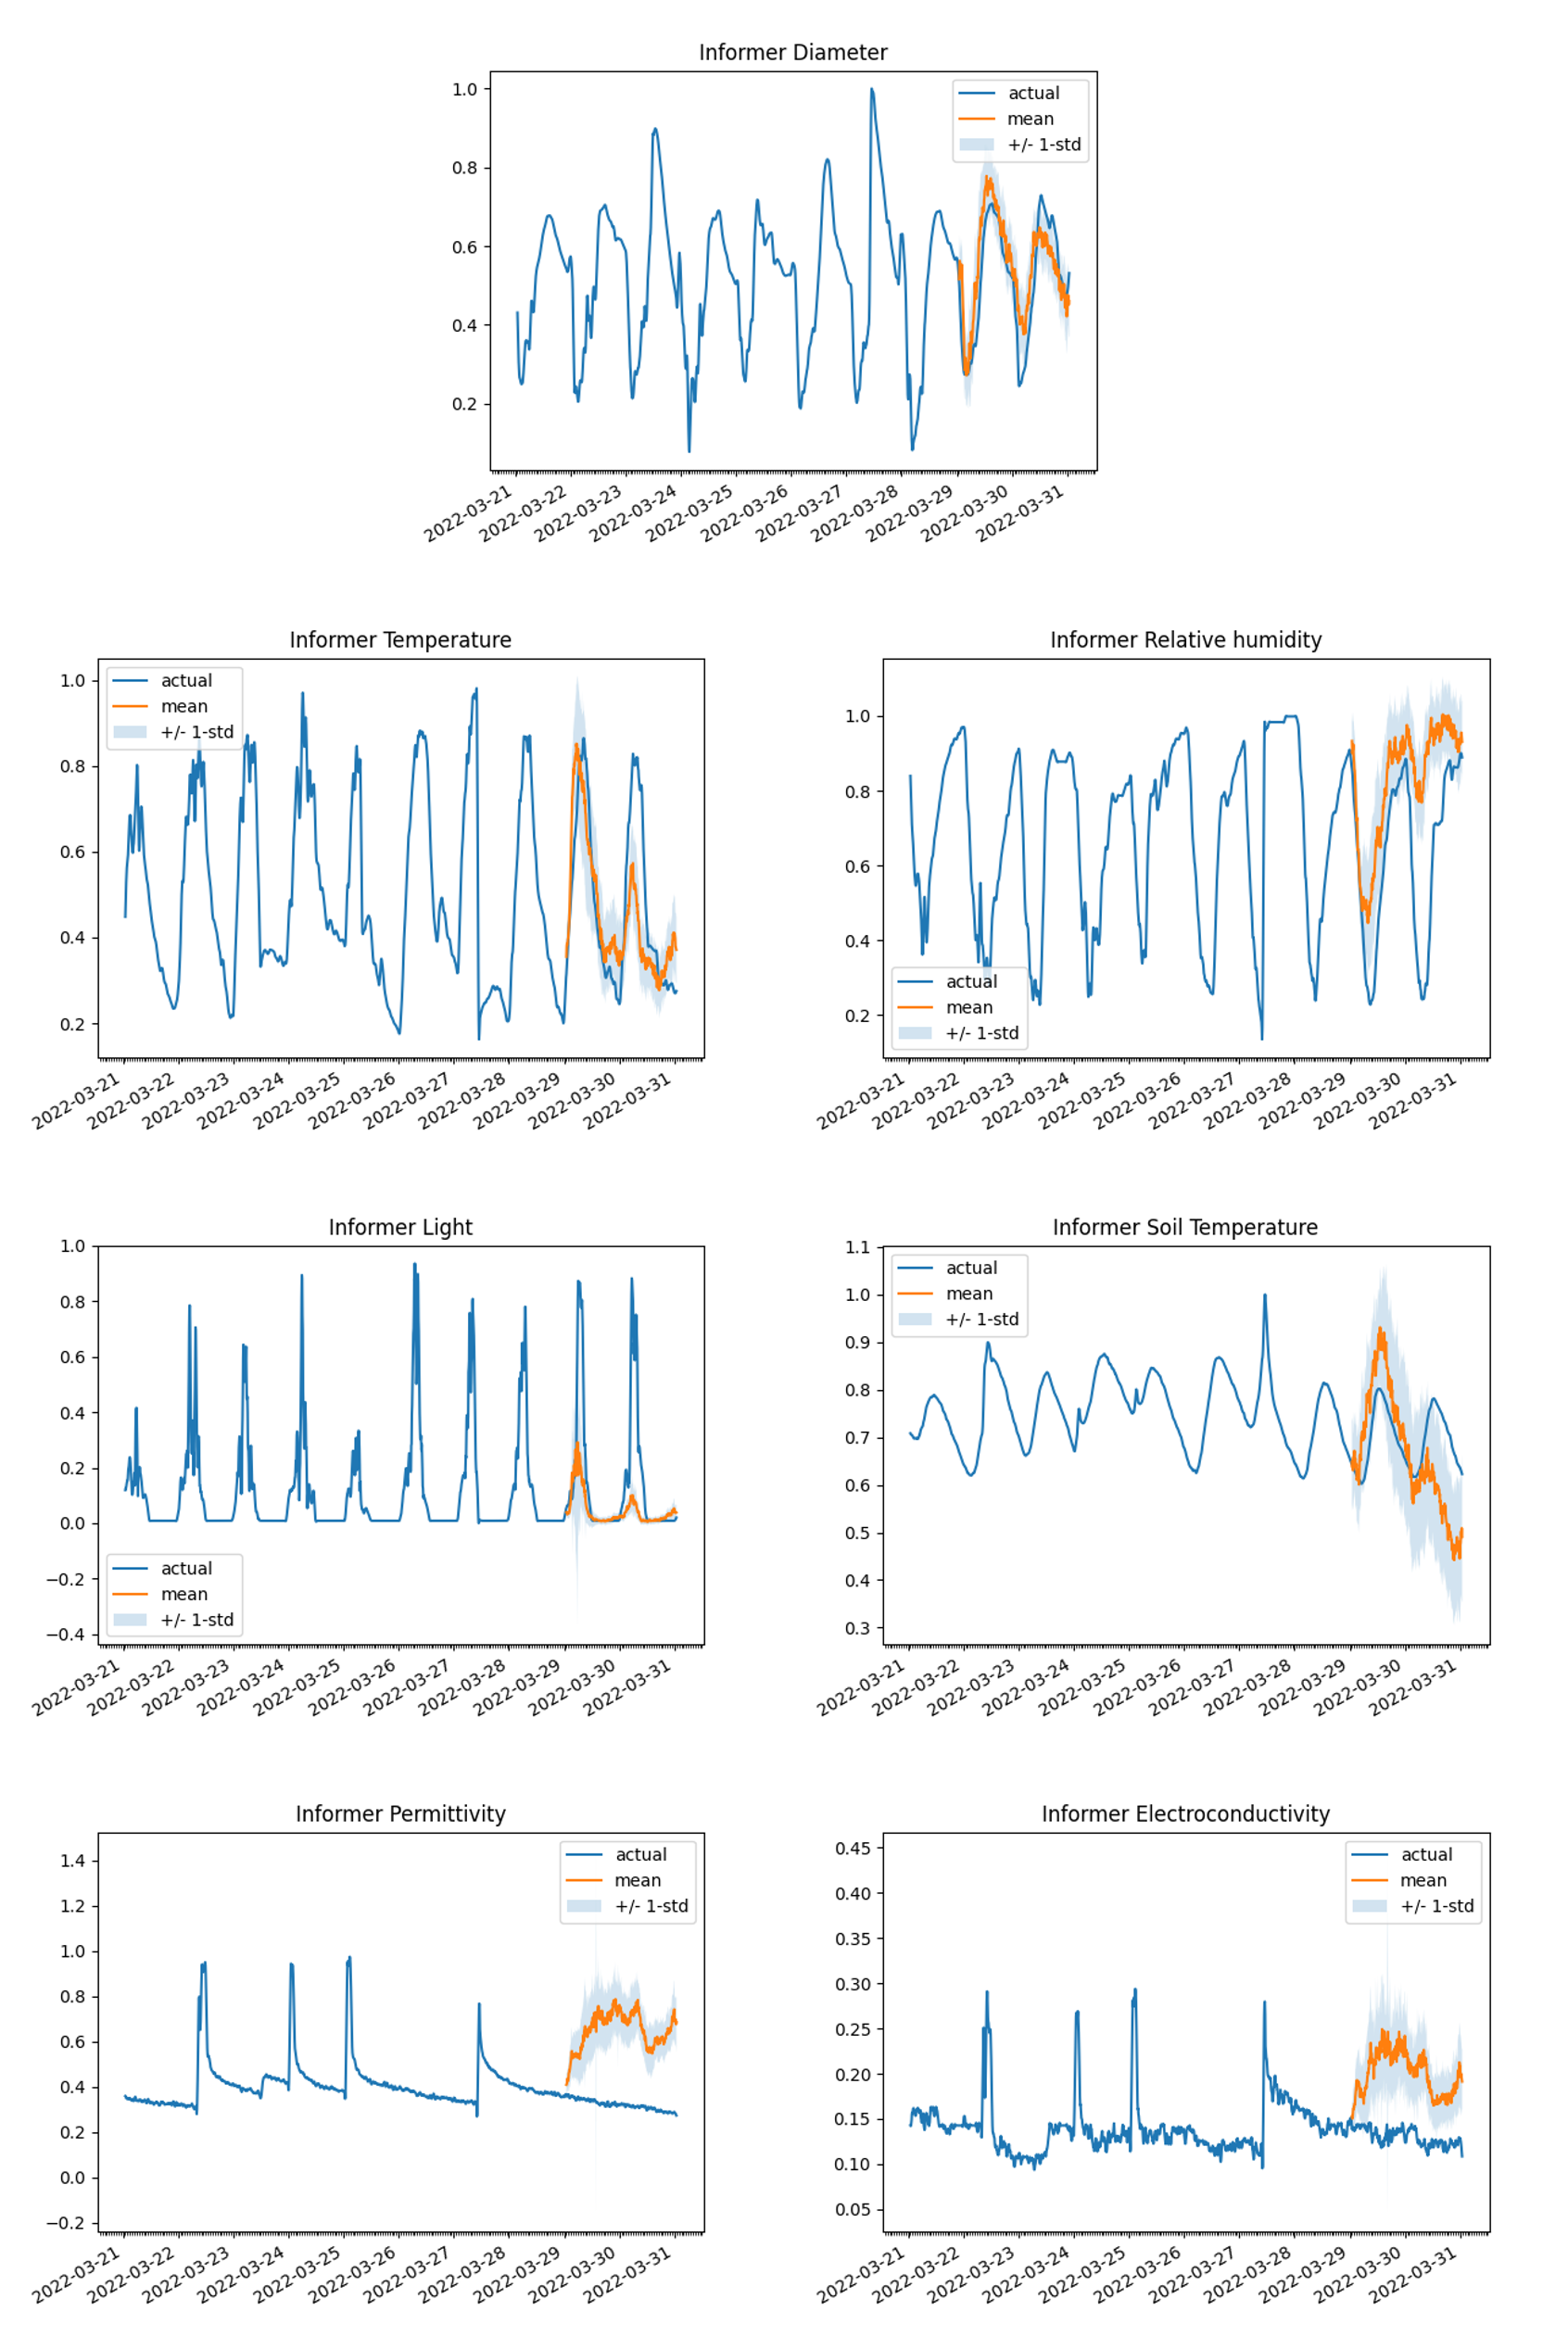
\includegraphics[width=15 cm]{6_ChapterResults/figuras/I20.png}
    \caption{Comparison between the predicted values generated by the I20 model and the actual observed values for the 7 variables over a two-day prediction horizon}
    \label{I20}
\end{figure}

\subsection{Autoformer}
The results for the Autoformer variant with modified Encoder Layers, Decoder Layers, and Dimensionality of the Transformer Layers, as shown in Tables \ref{A4_M} and \ref{A4_R}, reveal a range of performance outcomes when compared to the A11 model, which was used as the baseline for this experimental phase. Similar to the results observed with Transformer and Informer models, the performance across these Autoformer models is quite varied. Among all the models tested, A21 is considered the best due to its particularly strong performance in predicting the diameter. Figure \ref{A21} shows how the predictions from the A21 model align with the actual values, offering insight into the model's performance.

Additionally, as seen in Table \ref{A4_T}, increasing the number of layers leads to higher computational costs, consistent with the patterns observed in both Transformer and Informer models.



\begin{table}[]
    \centering
    \resizebox{\textwidth}{!}{%
    \begin{tabular}{ccccccccc}
    \multicolumn{9}{c}{\textbf{MSE   (Sorted by model)}}                                                                                                                                                                                                                          \\
    Model & Diameter                       & Electroconductivity            & Light                          & Permittivity                   & Relative\_humidity             & Soil\_Temperature              & Temperature                    & Mean                           \\
    A17   & \cellcolor[HTML]{8AC97D}-24.17 & \cellcolor[HTML]{F8696B}-35.47 & \cellcolor[HTML]{FED07F}-11.04 & \cellcolor[HTML]{F4E883}-24.02 & \cellcolor[HTML]{FED580}-16.68 & \cellcolor[HTML]{D5DF81}-21.84 & \cellcolor[HTML]{E3E382}-20.62 & \cellcolor[HTML]{F8E983}-21.98 \\
    A18   & \cellcolor[HTML]{F8696B}-15.94 & \cellcolor[HTML]{F8E983}-37.94 & \cellcolor[HTML]{89C97D}-11.33 & \cellcolor[HTML]{FFE583}-23.71 & \cellcolor[HTML]{F8696B}-12.72 & \cellcolor[HTML]{63BE7B}-24.18 & \cellcolor[HTML]{F8696B}-14.95 & \cellcolor[HTML]{F8696B}-20.11 \\
    A19   & \cellcolor[HTML]{FFE182}-19.12 & \cellcolor[HTML]{AFD37F}-38.86 & \cellcolor[HTML]{ADD37F}-11.29 & \cellcolor[HTML]{FCA477}-22.11 & \cellcolor[HTML]{FB9A75}-14.51 & \cellcolor[HTML]{82C77C}-23.53 & \cellcolor[HTML]{FCAE79}-17.51 & \cellcolor[HTML]{FCA877}-20.99 \\
    A20   & \cellcolor[HTML]{FB9874}-17.17 & \cellcolor[HTML]{FFE784}-37.79 & \cellcolor[HTML]{63BE7B}-11.39 & \cellcolor[HTML]{F8696B}-20.67 & \cellcolor[HTML]{ABD27F}-19.19 & \cellcolor[HTML]{FFDA81}-20.20 & \cellcolor[HTML]{FEC77D}-18.42 & \cellcolor[HTML]{FB9273}-20.69 \\
    A21   & \cellcolor[HTML]{63BE7B}-25.76 & \cellcolor[HTML]{FDB97B}-36.94 & \cellcolor[HTML]{F6E883}-11.19 & \cellcolor[HTML]{CFDD81}-24.59 & \cellcolor[HTML]{FDB67A}-15.54 & \cellcolor[HTML]{FFE383}-20.60 & \cellcolor[HTML]{FEEA83}-19.80 & \cellcolor[HTML]{E8E482}-22.06 \\
    A22   & \cellcolor[HTML]{F8E983}-19.68 & \cellcolor[HTML]{7EC57C}-39.47 & \cellcolor[HTML]{FFDD82}-11.10 & \cellcolor[HTML]{D1DD81}-24.56 & \cellcolor[HTML]{D5DF81}-18.34 & \cellcolor[HTML]{FFE182}-20.51 & \cellcolor[HTML]{FFEB84}-19.77 & \cellcolor[HTML]{FFE984}-21.92 \\
    A23   & \cellcolor[HTML]{FFDC82}-18.99 & \cellcolor[HTML]{FDBF7C}-37.04 & \cellcolor[HTML]{F8696B}-10.50 & \cellcolor[HTML]{FCA878}-22.22 & \cellcolor[HTML]{63BE7B}-20.63 & \cellcolor[HTML]{ECE582}-21.37 & \cellcolor[HTML]{63BE7B}-24.61 & \cellcolor[HTML]{CCDC81}-22.19 \\
    A24   & \cellcolor[HTML]{9BCE7E}-23.45 & \cellcolor[HTML]{63BE7B}-39.80 & \cellcolor[HTML]{FFE984}-11.17 & \cellcolor[HTML]{63BE7B}-26.22 & \cellcolor[HTML]{9FCF7E}-19.41 & \cellcolor[HTML]{F8696B}-15.08 & \cellcolor[HTML]{79C47C}-23.90 & \cellcolor[HTML]{63BE7B}-22.72
    \end{tabular}%
    }
    \caption{Mean Squared Errors (MSE) for different Autoformer models obtained by varying the number of Encoder Layers, Decoder Layers, and Dimensionality of the Transformer Layers, sorted by model}
    \label{A4_M}
    \end{table}



    
\begin{table}[]
    \centering
    \resizebox{\textwidth}{!}{%
    \begin{tabular}{ccccccccc}
    \multicolumn{9}{c}{\textbf{R2 (Sorted by model)}}                                                                                                                                                                                                                     \\
    Model & Diameter                      & Electroconductivity           & Light                         & Permittivity                   & Relative\_humidity            & Soil\_Temperature             & Temperature                  & Mean                          \\
    A17   & \cellcolor[HTML]{78C47D}0.83  & \cellcolor[HTML]{F8696B}-2.50 & \cellcolor[HTML]{FDD17F}-0.38 & \cellcolor[HTML]{F2E884}-7.65  & \cellcolor[HTML]{FEDE81}0.58  & \cellcolor[HTML]{C9DC81}-0.74 & \cellcolor[HTML]{D7E082}0.78 & \cellcolor[HTML]{E2E383}-1.30 \\
    A18   & \cellcolor[HTML]{F8696B}-0.15 & \cellcolor[HTML]{F8E984}-0.98 & \cellcolor[HTML]{89C97E}-0.29 & \cellcolor[HTML]{FEE683}-8.28  & \cellcolor[HTML]{F8696B}-0.06 & \cellcolor[HTML]{63BE7B}-0.02 & \cellcolor[HTML]{F8696B}0.18 & \cellcolor[HTML]{FEEB84}-1.37 \\
    A19   & \cellcolor[HTML]{FEE482}0.45  & \cellcolor[HTML]{A7D27F}-0.60 & \cellcolor[HTML]{ACD380}-0.30 & \cellcolor[HTML]{FBAF78}-12.44 & \cellcolor[HTML]{FBAB77}0.30  & \cellcolor[HTML]{7AC57D}-0.18 & \cellcolor[HTML]{FCBF7B}0.55 & \cellcolor[HTML]{FDC67D}-1.75 \\
    A20   & \cellcolor[HTML]{FBA376}0.14  & \cellcolor[HTML]{FEE783}-1.05 & \cellcolor[HTML]{63BE7B}-0.27 & \cellcolor[HTML]{F8696B}-17.70 & \cellcolor[HTML]{9CCF7F}0.76  & \cellcolor[HTML]{FEE282}-1.54 & \cellcolor[HTML]{FDD37F}0.63 & \cellcolor[HTML]{F8696B}-2.72 \\
    A21   & \cellcolor[HTML]{63BE7B}0.88  & \cellcolor[HTML]{FCC07B}-1.49 & \cellcolor[HTML]{F7E984}-0.33 & \cellcolor[HTML]{C7DB81}-6.60  & \cellcolor[HTML]{FDC67D}0.45  & \cellcolor[HTML]{FEE783}-1.31 & \cellcolor[HTML]{FFEB84}0.73 & \cellcolor[HTML]{94CC7E}-1.10 \\
    A22   & \cellcolor[HTML]{F3E884}0.51  & \cellcolor[HTML]{7AC57D}-0.39 & \cellcolor[HTML]{FEDD81}-0.36 & \cellcolor[HTML]{C9DC81}-6.65  & \cellcolor[HTML]{C7DB81}0.71  & \cellcolor[HTML]{FEE583}-1.37 & \cellcolor[HTML]{FEEA83}0.73 & \cellcolor[HTML]{63BE7B}-0.97 \\
    A23   & \cellcolor[HTML]{FEE082}0.43  & \cellcolor[HTML]{FDC67C}-1.43 & \cellcolor[HTML]{F8696B}-0.56 & \cellcolor[HTML]{FCB379}-12.10 & \cellcolor[HTML]{63BE7B}0.83  & \cellcolor[HTML]{E5E483}-0.94 & \cellcolor[HTML]{63BE7B}0.91 & \cellcolor[HTML]{FCBE7B}-1.84 \\
    A24   & \cellcolor[HTML]{84C87D}0.80  & \cellcolor[HTML]{63BE7B}-0.29 & \cellcolor[HTML]{FEE883}-0.34 & \cellcolor[HTML]{63BE7B}-4.21  & \cellcolor[HTML]{92CC7E}0.77  & \cellcolor[HTML]{F8696B}-7.25 & \cellcolor[HTML]{71C37C}0.90 & \cellcolor[HTML]{FEEA83}-1.37
    \end{tabular}%
    }
    \caption{R-squared (R²) for different Autoformer models obtained by varying the number of Encoder Layers, Decoder Layers, and Dimensionality of the Transformer Layers, sorted by model}
    \label{A4_R}
    \end{table}


    

\begin{table}[]
    \begin{tabular}{ccccc}
    \multicolumn{2}{c}{\textbf{Training   Time (Sorted by model)}} &  & \multicolumn{2}{c}{\textbf{Training Time (Sorted   by training time)}} \\
    Model             & Training time {[}s{]}                      &  & Model                 & Training time {[}s{]}                          \\
    A17               & \cellcolor[HTML]{63BE7B}182.03             &  & A17                   & \cellcolor[HTML]{63BE7B}182.03                 \\
    A18               & \cellcolor[HTML]{E5E382}276.08             &  & A20                   & \cellcolor[HTML]{97CD7E}219.77                 \\
    A19               & \cellcolor[HTML]{FCB279}426.11             &  & A22                   & \cellcolor[HTML]{CDDC81}258.71                 \\
    A20               & \cellcolor[HTML]{97CD7E}219.77             &  & A18                   & \cellcolor[HTML]{E5E382}276.08                 \\
    A21               & \cellcolor[HTML]{FFE483}312.17             &  & A21                   & \cellcolor[HTML]{FFE483}312.17                 \\
    A22               & \cellcolor[HTML]{CDDC81}258.71             &  & A23                   & \cellcolor[HTML]{FECC7E}367.55                 \\
    A23               & \cellcolor[HTML]{FECC7E}367.55             &  & A19                   & \cellcolor[HTML]{FCB279}426.11                 \\
    A24               & \cellcolor[HTML]{F8696B}592.64             &  & A24                   & \cellcolor[HTML]{F8696B}592.64                
    \end{tabular}
    \caption{Training times for different Autoformer models obtained by varying the number of Encoder Layers, Decoder Layers, and Dimensionality of the Transformer Layers, sorted by model and training time values}
    \label{A4_T}
    \end{table}

\begin{figure}[htbp]
    \centering
    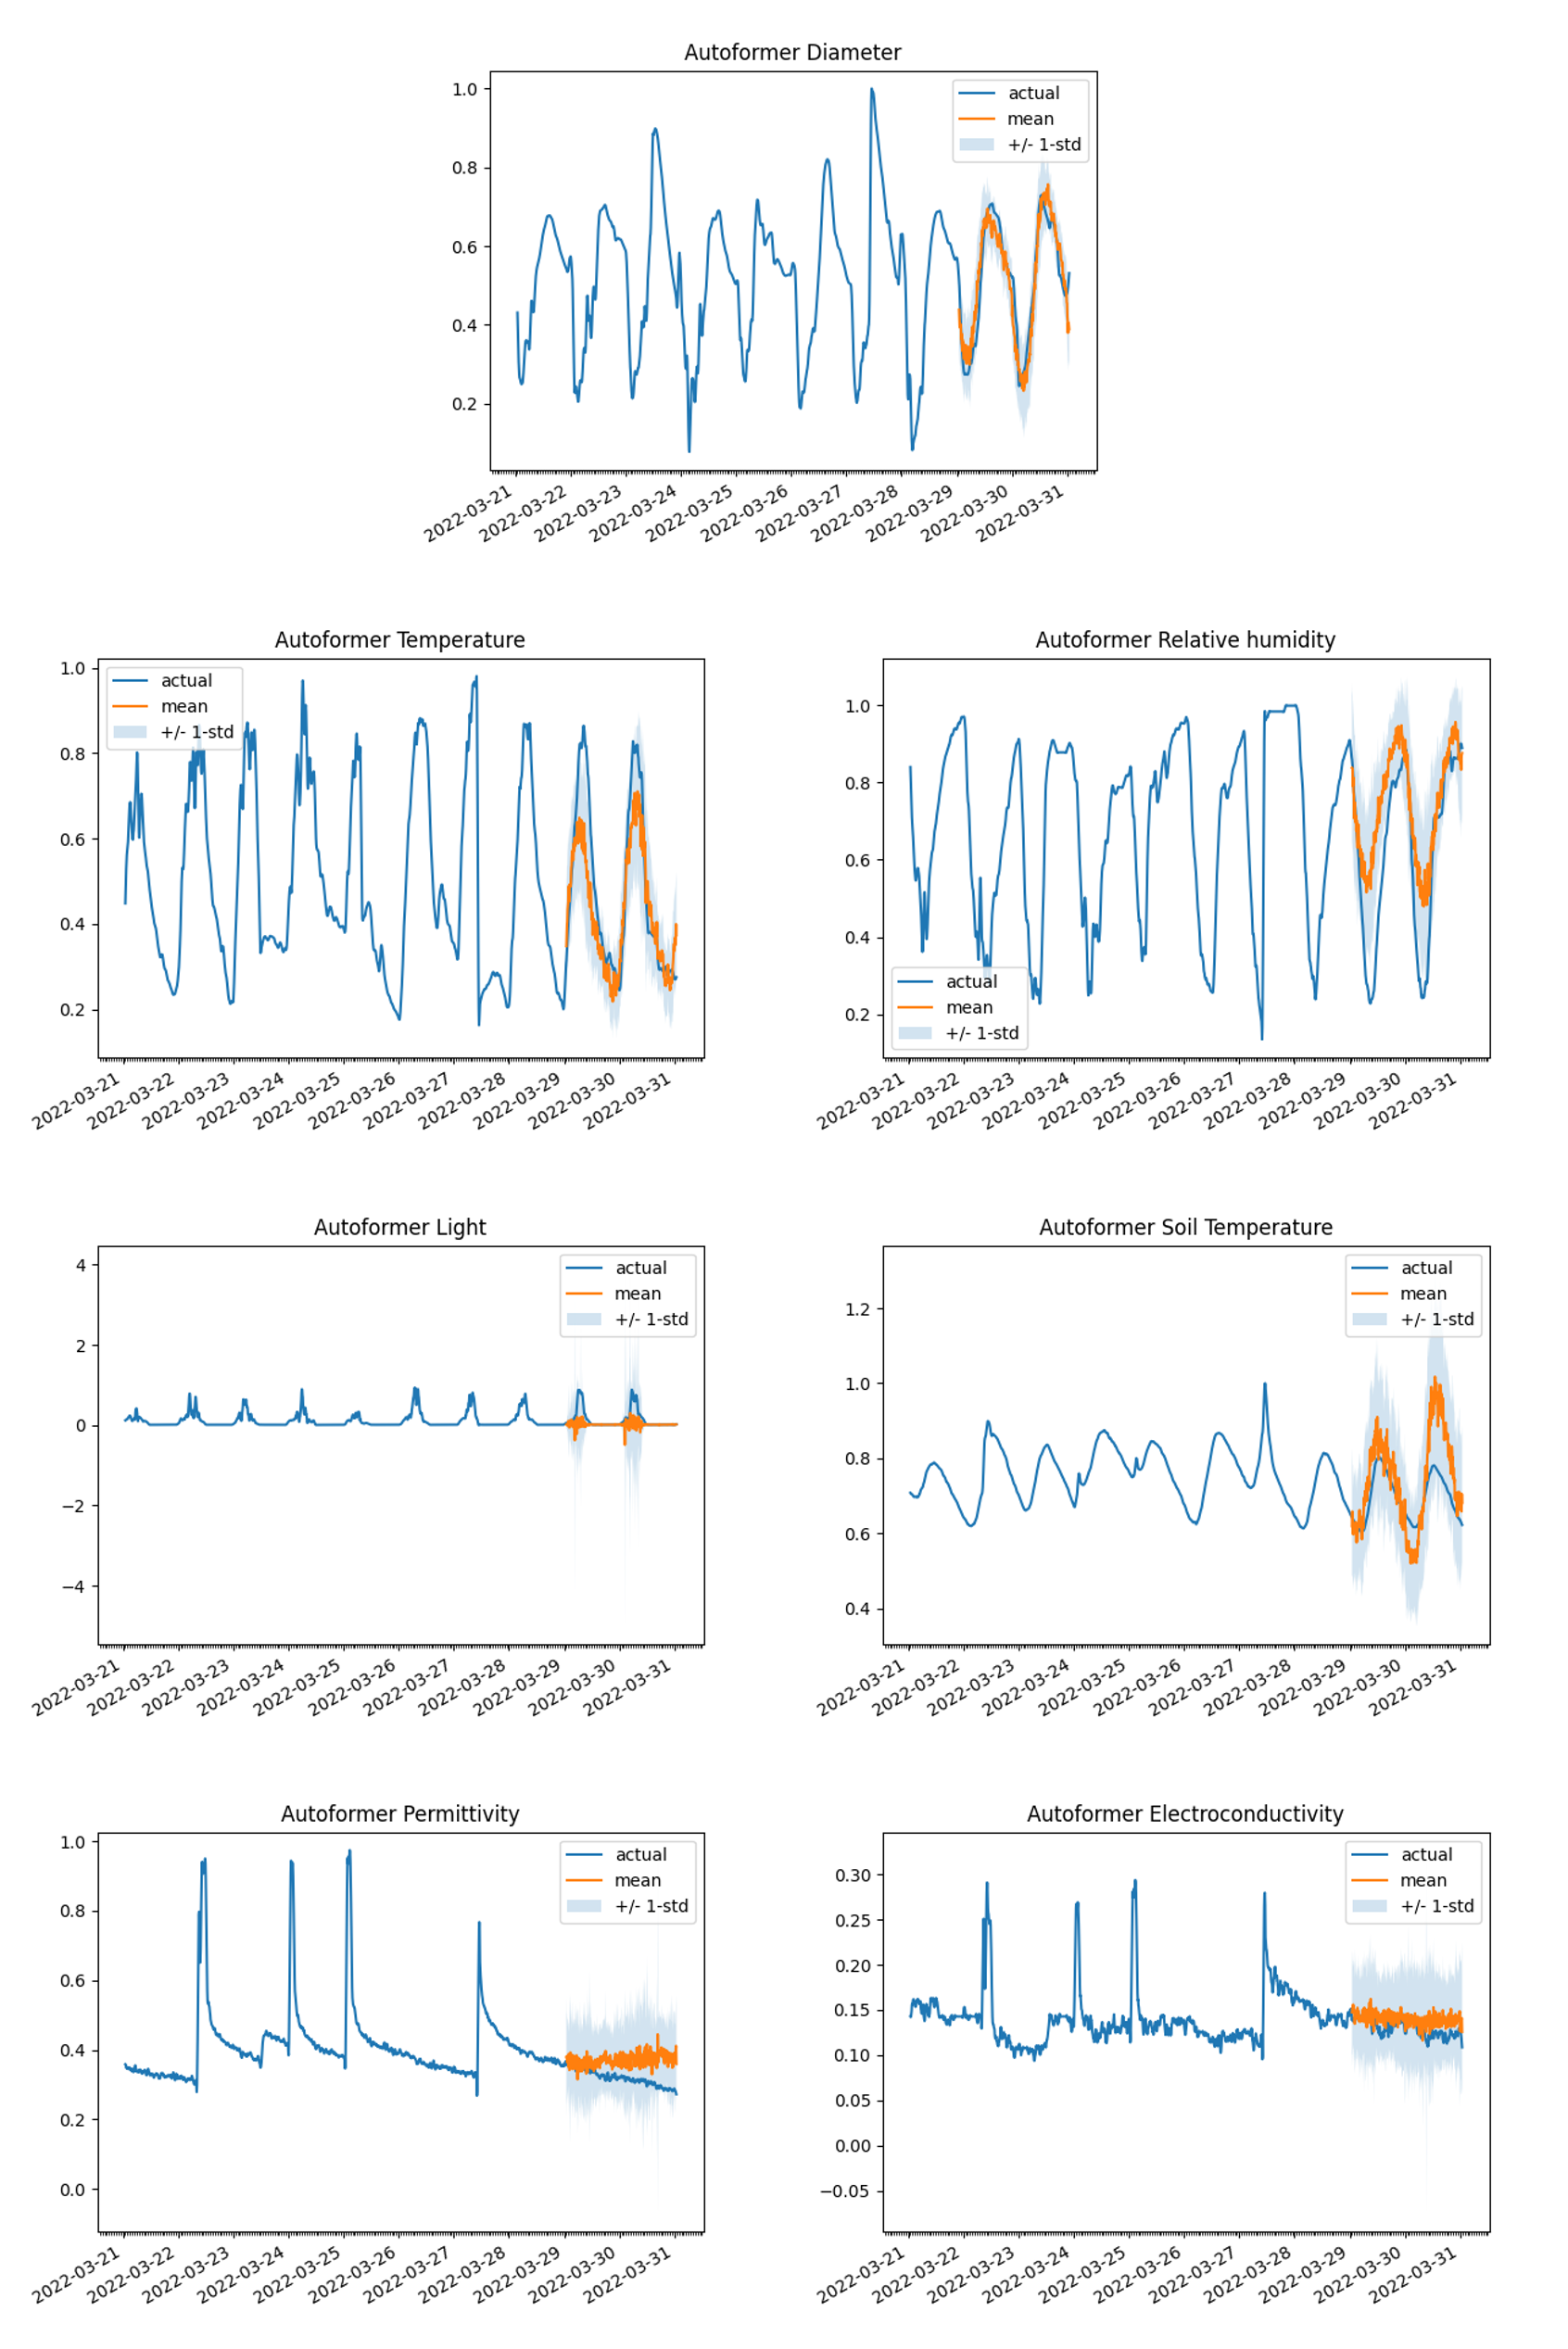
\includegraphics[width=15 cm]{6_ChapterResults/figuras/A21.png}
    \caption{Comparison between the predicted values generated by the A21 model and the actual observed values for the 7 variables over a two-day prediction horizon}
    \label{A21}
\end{figure}

\section{Effect of Batch Size and Number of Epochs}
In this section, we present the results of experiments conducted by altering the Batch Size and Number of Epochs across different model variants. These hyperparameters play a crucial role in determining the model's learning process, with Batch Size influencing the number of samples processed before the model’s weights are updated, and Number of Epochs determining the number of times the model iterates over the entire training dataset.

\subsection{Transformer}
The results for the Transformer variant with modified Batch Size and Number of Epochs, as shown in Tables \ref{T5_M} and \ref{T5_R}, exhibit diverse outcomes compared to the T15 model, which was used as the baseline for this experimental phase. Generally, increasing the Batch Size and Number of Epochs leads to improved performance, suggesting that these hyperparameters are crucial for the scalability of Transformer models.

One of the most notable models developed during this phase is the T30 model, which stands out for its strong performance. A detailed comparison of its predictions against the actual values of the seven variables is illustrated in Figure \ref{T30}, demonstrating the model's effectiveness in this experimental setup.

However, as observed in Table \ref{T5_T}, increasing the Batch Size and Number of Epochs also results in higher computational costs and, consequently, longer training times. This trade-off between performance gains and computational efficiency highlights the importance of carefully tuning these hyperparameters to balance accuracy with practical training times.
    

    

\begin{table}[]
    \centering
    \resizebox{\textwidth}{!}{%
    \begin{tabular}{ccccccccc}
    \multicolumn{9}{c}{\textbf{MSE   (Sorted by model)}}                                                                                                                                                                                                                          \\
    Model & Diameter                       & Electroconductivity            & Light                          & Permittivity                   & Relative Humidity              & Soil Temperature               & Temperature                    & Mean                           \\
    T25   & \cellcolor[HTML]{E9E482}-21.84 & \cellcolor[HTML]{F8696B}-19.67 & \cellcolor[HTML]{FDB67A}-13.20 & \cellcolor[HTML]{F8696B}-9.52  & \cellcolor[HTML]{FFEA84}-15.57 & \cellcolor[HTML]{F8696B}-4.95  & \cellcolor[HTML]{FDEA83}-18.15 & \cellcolor[HTML]{F8696B}-14.70 \\
    T26   & \cellcolor[HTML]{F8696B}-17.02 & \cellcolor[HTML]{64BE7B}-35.76 & \cellcolor[HTML]{F8696B}-12.65 & \cellcolor[HTML]{82C67C}-24.94 & \cellcolor[HTML]{F8696B}-9.38  & \cellcolor[HTML]{FFE683}-15.36 & \cellcolor[HTML]{F8696B}-11.96 & \cellcolor[HTML]{FFE383}-18.15 \\
    T27   & \cellcolor[HTML]{FFE082}-21.05 & \cellcolor[HTML]{63BE7B}-35.87 & \cellcolor[HTML]{97CD7E}-14.49 & \cellcolor[HTML]{63BE7B}-25.82 & \cellcolor[HTML]{FBEA83}-15.73 & \cellcolor[HTML]{C3D980}-21.04 & \cellcolor[HTML]{A8D27F}-20.66 & \cellcolor[HTML]{63BE7B}-22.09 \\
    T28   & \cellcolor[HTML]{A8D27F}-23.01 & \cellcolor[HTML]{FFE383}-25.19 & \cellcolor[HTML]{FA8871}-12.87 & \cellcolor[HTML]{7FC67C}-25.03 & \cellcolor[HTML]{FCAF79}-12.71 & \cellcolor[HTML]{F9E983}-16.24 & \cellcolor[HTML]{FCAF79}-15.25 & \cellcolor[HTML]{F5E883}-18.61 \\
    T29   & \cellcolor[HTML]{FCB179}-19.46 & \cellcolor[HTML]{F9E983}-25.98 & \cellcolor[HTML]{D2DE81}-13.97 & \cellcolor[HTML]{FA8972}-12.42 & \cellcolor[HTML]{E3E282}-16.29 & \cellcolor[HTML]{FB9975}-8.94  & \cellcolor[HTML]{FFEB84}-18.08 & \cellcolor[HTML]{FCA777}-16.45 \\
    T30   & \cellcolor[HTML]{63BE7B}-24.28 & \cellcolor[HTML]{FEC87E}-23.97 & \cellcolor[HTML]{63BE7B}-14.94 & \cellcolor[HTML]{FDC57D}-17.90 & \cellcolor[HTML]{63BE7B}-19.24 & \cellcolor[HTML]{63BE7B}-29.52 & \cellcolor[HTML]{63BE7B}-22.70 & \cellcolor[HTML]{6FC17B}-21.79
    \end{tabular}%
    }
    \caption{Mean Squared Errors (MSE) for different Transformer models obtained by varying the Batch Size and Number of Epochs values, sorted by model}
    \label{T5_M}
    \end{table}


    

\begin{table}[]
    \centering
    \resizebox{\textwidth}{!}{%
    \begin{tabular}{ccccccccc}
    \multicolumn{9}{c}{\textbf{R2 (Sorted by model)}}                                                                                                                                                                                                                         \\
    Model & Diameter                     & Electroconductivity             & Light                        & Permittivity                    & Relative\_humidity            & Soil\_Temperature              & Temperature                   & Mean                           \\
    T25   & \cellcolor[HTML]{E3E383}0.70 & \cellcolor[HTML]{F8696B}-131.83 & \cellcolor[HTML]{FCBA7A}0.16 & \cellcolor[HTML]{F8696B}-242.90 & \cellcolor[HTML]{FEEA83}0.45  & \cellcolor[HTML]{F8696B}-83.96 & \cellcolor[HTML]{FDEB84}0.61  & \cellcolor[HTML]{F8696B}-65.25 \\
    T26   & \cellcolor[HTML]{F8696B}0.11 & \cellcolor[HTML]{64BF7C}-2.27   & \cellcolor[HTML]{F8696B}0.05 & \cellcolor[HTML]{70C27C}-6.00   & \cellcolor[HTML]{F8696B}-1.28 & \cellcolor[HTML]{FEE983}-6.74  & \cellcolor[HTML]{F8696B}-0.62 & \cellcolor[HTML]{82C77D}-2.39  \\
    T27   & \cellcolor[HTML]{FEE482}0.65 & \cellcolor[HTML]{63BE7B}-2.19   & \cellcolor[HTML]{92CC7E}0.38 & \cellcolor[HTML]{63BE7B}-4.72   & \cellcolor[HTML]{FBEA84}0.47  & \cellcolor[HTML]{8DCA7E}-1.09  & \cellcolor[HTML]{95CD7E}0.78  & \cellcolor[HTML]{63BE7B}-0.82  \\
    T28   & \cellcolor[HTML]{9DCF7F}0.77 & \cellcolor[HTML]{FEE683}-36.29  & \cellcolor[HTML]{F98A71}0.10 & \cellcolor[HTML]{6FC27C}-5.87   & \cellcolor[HTML]{FCC47C}-0.06 & \cellcolor[HTML]{EFE784}-5.32  & \cellcolor[HTML]{FCC47C}0.24  & \cellcolor[HTML]{D3DF82}-6.63  \\
    T29   & \cellcolor[HTML]{FCC07B}0.49 & \cellcolor[HTML]{F0E784}-30.12  & \cellcolor[HTML]{CDDD82}0.30 & \cellcolor[HTML]{FBAE78}-123.95 & \cellcolor[HTML]{D9E082}0.54  & \cellcolor[HTML]{FCBE7B}-32.95 & \cellcolor[HTML]{FEEA83}0.60  & \cellcolor[HTML]{FCC27C}-26.44 \\
    T30   & \cellcolor[HTML]{63BE7B}0.83 & \cellcolor[HTML]{FDD780}-48.35  & \cellcolor[HTML]{63BE7B}0.44 & \cellcolor[HTML]{FEE282}-34.42  & \cellcolor[HTML]{63BE7B}0.77  & \cellcolor[HTML]{63BE7B}0.70   & \cellcolor[HTML]{63BE7B}0.86  & \cellcolor[HTML]{FEE582}-11.31
    \end{tabular}%
    }
    \caption{R-squared (R²) for different Transformer models obtained by varying the Batch Size and Number of Epochs values, sorted by model}
    \label{T5_R}
    \end{table}



    
\begin{table}[]
    \begin{tabular}{ccccc}
    \multicolumn{2}{c}{\textbf{Training   Time (Sorted by model)}} &  & \multicolumn{2}{c}{\textbf{Training Time (Sorted   by training time)}} \\
    Model             & Training time {[}s{]}                      &  & Model                 & Training time {[}s{]}                          \\
    T25               & \cellcolor[HTML]{63BE7B}130.65             &  & T25                   & \cellcolor[HTML]{63BE7B}130.65                 \\
    T26               & \cellcolor[HTML]{E3E382}387.01             &  & T27                   & \cellcolor[HTML]{9DCF7E}248.18                 \\
    T27               & \cellcolor[HTML]{9DCF7E}248.18             &  & T26                   & \cellcolor[HTML]{E3E382}387.01                 \\
    T28               & \cellcolor[HTML]{FDC67D}756.21             &  & T29                   & \cellcolor[HTML]{FFE583}495.93                 \\
    T29               & \cellcolor[HTML]{FFE583}495.93             &  & T28                   & \cellcolor[HTML]{FDC67D}756.21                 \\
    T30               & \cellcolor[HTML]{F8696B}1542.75            &  & T30                   & \cellcolor[HTML]{F8696B}1542.75               
    \end{tabular}
    \caption{Training times for different Transformer models obtained by varying the Batch Size and Number of Epochs values, sorted by model and training time values}
    \label{T5_T}
    \end{table}

\begin{figure}[htbp]
    \centering
    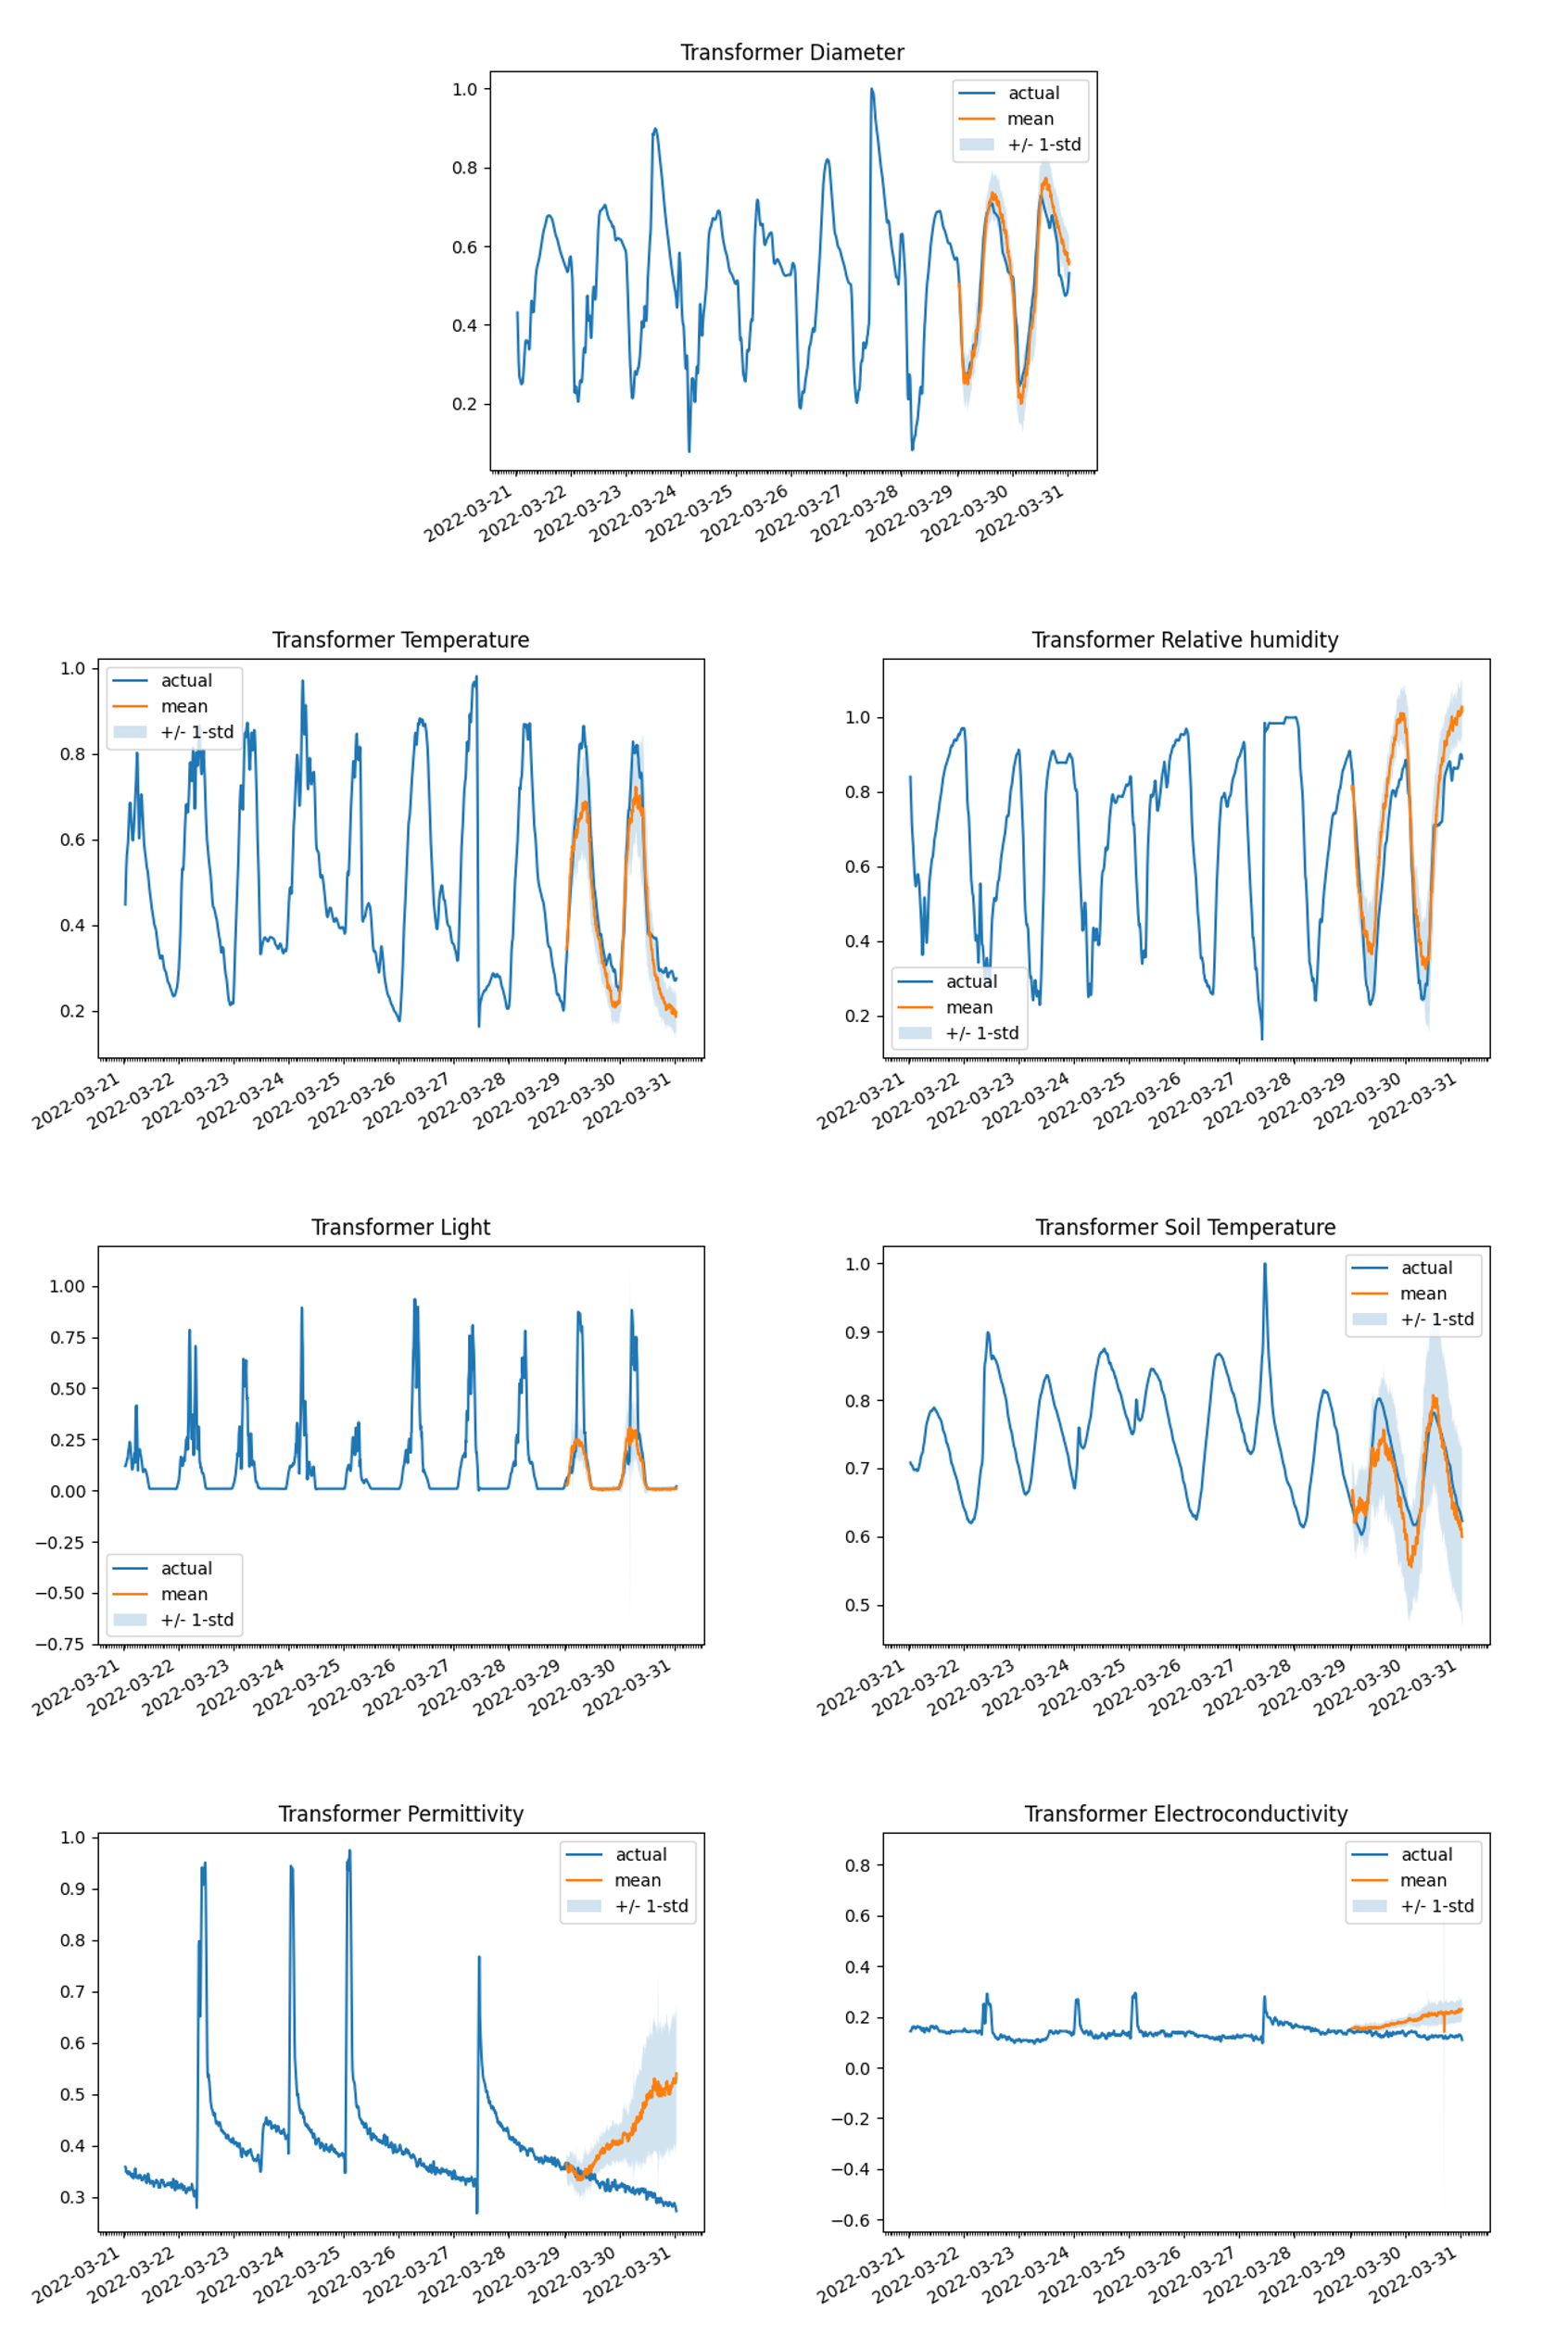
\includegraphics[width=15 cm]{6_ChapterResults/figuras/T30.png}
    \caption{Comparison between the predicted values generated by the T30 model and the actual observed values for the 7 variables over a two-day prediction horizon}
    \label{T30}
\end{figure}

\subsection{Informer}
The results for the Informer variant with modified Batch Size and Number of Epochs, as shown in Tables \ref{I5_M} and \ref{I5_R}, display varied outcomes compared to the I20 model, which served as the baseline for this experimental phase. Generally, increasing the Batch Size and Number of Epochs leads to improved performance, similar to what was observed with the Transformer models. This indicates that these hyperparameters are also important for optimizing the Informer's predictive capabilities.

Among the models evaluated in this phase, the I30 model emerged as a top performer, showing remarkable accuracy in predictions. Figure \ref{I30} provides a visual comparison between the predicted and actual values of the seven variables, underscoring the model's success in this phase of the experiment.

However, as seen in Table \ref{I5_T}, increasing the Batch Size and Number of Epochs results in higher computational costs and longer training times. Despite this, the Informer remains more efficient compared to the Transformer, maintaining better computational efficiency even with these adjustments.
    

    
\begin{table}[]
    \centering
    \resizebox{\textwidth}{!}{%
    \begin{tabular}{ccccccccc}
    \multicolumn{9}{c}{\textbf{MSE   (Sorted by model)}}                                                                                                                                                                                                                          \\
    Model & Diameter                       & Electroconductivity            & Light                          & Permittivity                   & Relative\_humidity             & Soil\_Temperature              & Temperature                    & Mean                           \\
    I25   & \cellcolor[HTML]{F8696B}-16.77 & \cellcolor[HTML]{FCAA78}-29.75 & \cellcolor[HTML]{FDBD7B}-12.62 & \cellcolor[HTML]{FB9975}-15.51 & \cellcolor[HTML]{F8696B}-11.20 & \cellcolor[HTML]{FB9073}-10.05 & \cellcolor[HTML]{F8696B}-9.60  & \cellcolor[HTML]{F8696B}-15.07 \\
    I26   & \cellcolor[HTML]{C2D980}-22.58 & \cellcolor[HTML]{FFE383}-35.67 & \cellcolor[HTML]{A3D07E}-13.74 & \cellcolor[HTML]{63BE7B}-29.67 & \cellcolor[HTML]{88C87D}-16.02 & \cellcolor[HTML]{98CD7E}-26.51 & \cellcolor[HTML]{AAD27F}-18.55 & \cellcolor[HTML]{6DC17B}-23.25 \\
    I27   & \cellcolor[HTML]{FEC97E}-19.74 & \cellcolor[HTML]{DBE081}-37.34 & \cellcolor[HTML]{F8696B}-12.19 & \cellcolor[HTML]{C5DA80}-26.03 & \cellcolor[HTML]{E2E282}-13.88 & \cellcolor[HTML]{F8696B}-6.48  & \cellcolor[HTML]{FB9474}-11.65 & \cellcolor[HTML]{FED380}-18.19 \\
    I28   & \cellcolor[HTML]{63BE7B}-25.39 & \cellcolor[HTML]{F8696B}-23.12 & \cellcolor[HTML]{E5E382}-13.11 & \cellcolor[HTML]{F8696B}-10.63 & \cellcolor[HTML]{FDBE7C}-12.50 & \cellcolor[HTML]{A3D07E}-25.60 & \cellcolor[HTML]{A4D07E}-18.75 & \cellcolor[HTML]{FFDC82}-18.44 \\
    I29   & \cellcolor[HTML]{FDC27D}-19.52 & \cellcolor[HTML]{63BE7B}-40.22 & \cellcolor[HTML]{FCB079}-12.55 & \cellcolor[HTML]{C2D980}-26.13 & \cellcolor[HTML]{FDC07C}-12.53 & \cellcolor[HTML]{FB9F76}-11.41 & \cellcolor[HTML]{FCB37A}-13.11 & \cellcolor[HTML]{EFE683}-19.35 \\
    I30   & \cellcolor[HTML]{DBE081}-21.86 & \cellcolor[HTML]{AAD27F}-38.52 & \cellcolor[HTML]{63BE7B}-14.36 & \cellcolor[HTML]{FED780}-21.75 & \cellcolor[HTML]{63BE7B}-16.90 & \cellcolor[HTML]{63BE7B}-30.65 & \cellcolor[HTML]{63BE7B}-20.88 & \cellcolor[HTML]{63BE7B}-23.56
    \end{tabular}%
    }
    \caption{Mean Squared Errors (MSE) for different Informer models obtained by varying the Batch Size and Number of Epochs values, sorted by model}
    \label{I5_M}
    \end{table}


    
\begin{table}[]
    \centering
    \resizebox{\textwidth}{!}{%
    \begin{tabular}{ccccccccc}
    \multicolumn{9}{c}{\textbf{R2 (Sorted by model)}}                                                                                                                                                                                                                         \\
    Model & Diameter                     & Electroconductivity            & Light                         & Permittivity                    & Relative\_humidity            & Soil\_Temperature              & Temperature                   & Mean                           \\
    I25   & \cellcolor[HTML]{F8696B}0.05 & \cellcolor[HTML]{FDD37F}-12.06 & \cellcolor[HTML]{FCBF7B}0.05  & \cellcolor[HTML]{FCC57C}-60.38  & \cellcolor[HTML]{F8696B}-0.50 & \cellcolor[HTML]{FCC07B}-25.26 & \cellcolor[HTML]{F8696B}-1.80 & \cellcolor[HTML]{FDC67D}-14.27 \\
    I26   & \cellcolor[HTML]{ACD380}0.75 & \cellcolor[HTML]{FEE983}-2.34  & \cellcolor[HTML]{9DCF7F}0.26  & \cellcolor[HTML]{63BE7B}-1.36   & \cellcolor[HTML]{7DC67D}0.51  & \cellcolor[HTML]{69C07C}0.41   & \cellcolor[HTML]{8ACA7E}0.64  & \cellcolor[HTML]{63BE7B}-0.16  \\
    I27   & \cellcolor[HTML]{FDD57F}0.52 & \cellcolor[HTML]{CCDD82}-1.27  & \cellcolor[HTML]{F8696B}-0.06 & \cellcolor[HTML]{A2D17F}-4.45   & \cellcolor[HTML]{D6E082}0.19  & \cellcolor[HTML]{F8696B}-58.73 & \cellcolor[HTML]{FBAD78}-0.75 & \cellcolor[HTML]{FEDD81}-9.22  \\
    I28   & \cellcolor[HTML]{63BE7B}0.87 & \cellcolor[HTML]{F8696B}-59.13 & \cellcolor[HTML]{E2E383}0.15  & \cellcolor[HTML]{F8696B}-188.09 & \cellcolor[HTML]{FCC57C}-0.11 & \cellcolor[HTML]{6CC17C}0.27   & \cellcolor[HTML]{86C97E}0.66  & \cellcolor[HTML]{F8696B}-35.05 \\
    I29   & \cellcolor[HTML]{FDCF7E}0.50 & \cellcolor[HTML]{63BE7B}-0.17  & \cellcolor[HTML]{FBB279}0.03  & \cellcolor[HTML]{A0D07F}-4.33   & \cellcolor[HTML]{FDC77D}-0.11 & \cellcolor[HTML]{FDD27F}-18.22 & \cellcolor[HTML]{FDCD7E}-0.25 & \cellcolor[HTML]{B2D580}-3.22  \\
    I30   & \cellcolor[HTML]{C7DB81}0.71 & \cellcolor[HTML]{99CE7F}-0.73  & \cellcolor[HTML]{63BE7B}0.36  & \cellcolor[HTML]{FEE783}-13.59  & \cellcolor[HTML]{63BE7B}0.60  & \cellcolor[HTML]{63BE7B}0.77   & \cellcolor[HTML]{63BE7B}0.79  & \cellcolor[HTML]{88C97E}-1.59 
    \end{tabular}%
    }
    \caption{R-squared (R²) for different Informer models obtained by varying the Batch Size and Number of Epochs values, sorted by model}
    \label{I5_R}
    \end{table}



\begin{table}[]
    \begin{tabular}{ccccc}
    \multicolumn{2}{c}{\textbf{Training   Time (Sorted by model)}} &  & \multicolumn{2}{c}{\textbf{Training Time (Sorted   by training time)}} \\
    Model             & Training time {[}s{]}                      &  & Model                 & Training time {[}s{]}                          \\
    I25               & \cellcolor[HTML]{63BE7B}59.53              &  & I25                   & \cellcolor[HTML]{63BE7B}59.53                  \\
    I26               & \cellcolor[HTML]{FFE784}163.53             &  & I27                   & \cellcolor[HTML]{90CB7D}86.82                  \\
    I27               & \cellcolor[HTML]{90CB7D}86.82              &  & I29                   & \cellcolor[HTML]{EDE582}142.6                  \\
    I28               & \cellcolor[HTML]{FDBC7B}255.43             &  & I26                   & \cellcolor[HTML]{FFE784}163.53                 \\
    I29               & \cellcolor[HTML]{EDE582}142.6              &  & I28                   & \cellcolor[HTML]{FDBC7B}255.43                 \\
    I30               & \cellcolor[HTML]{F8696B}432.91             &  & I30                   & \cellcolor[HTML]{F8696B}432.91                
    \end{tabular}
    \caption{Training times for different Informer models obtained by varying the Batch Size and Number of Epochs values, sorted by model and training time values}
    \label{I5_T}
    \end{table}

\begin{figure}[htbp]
    \centering
    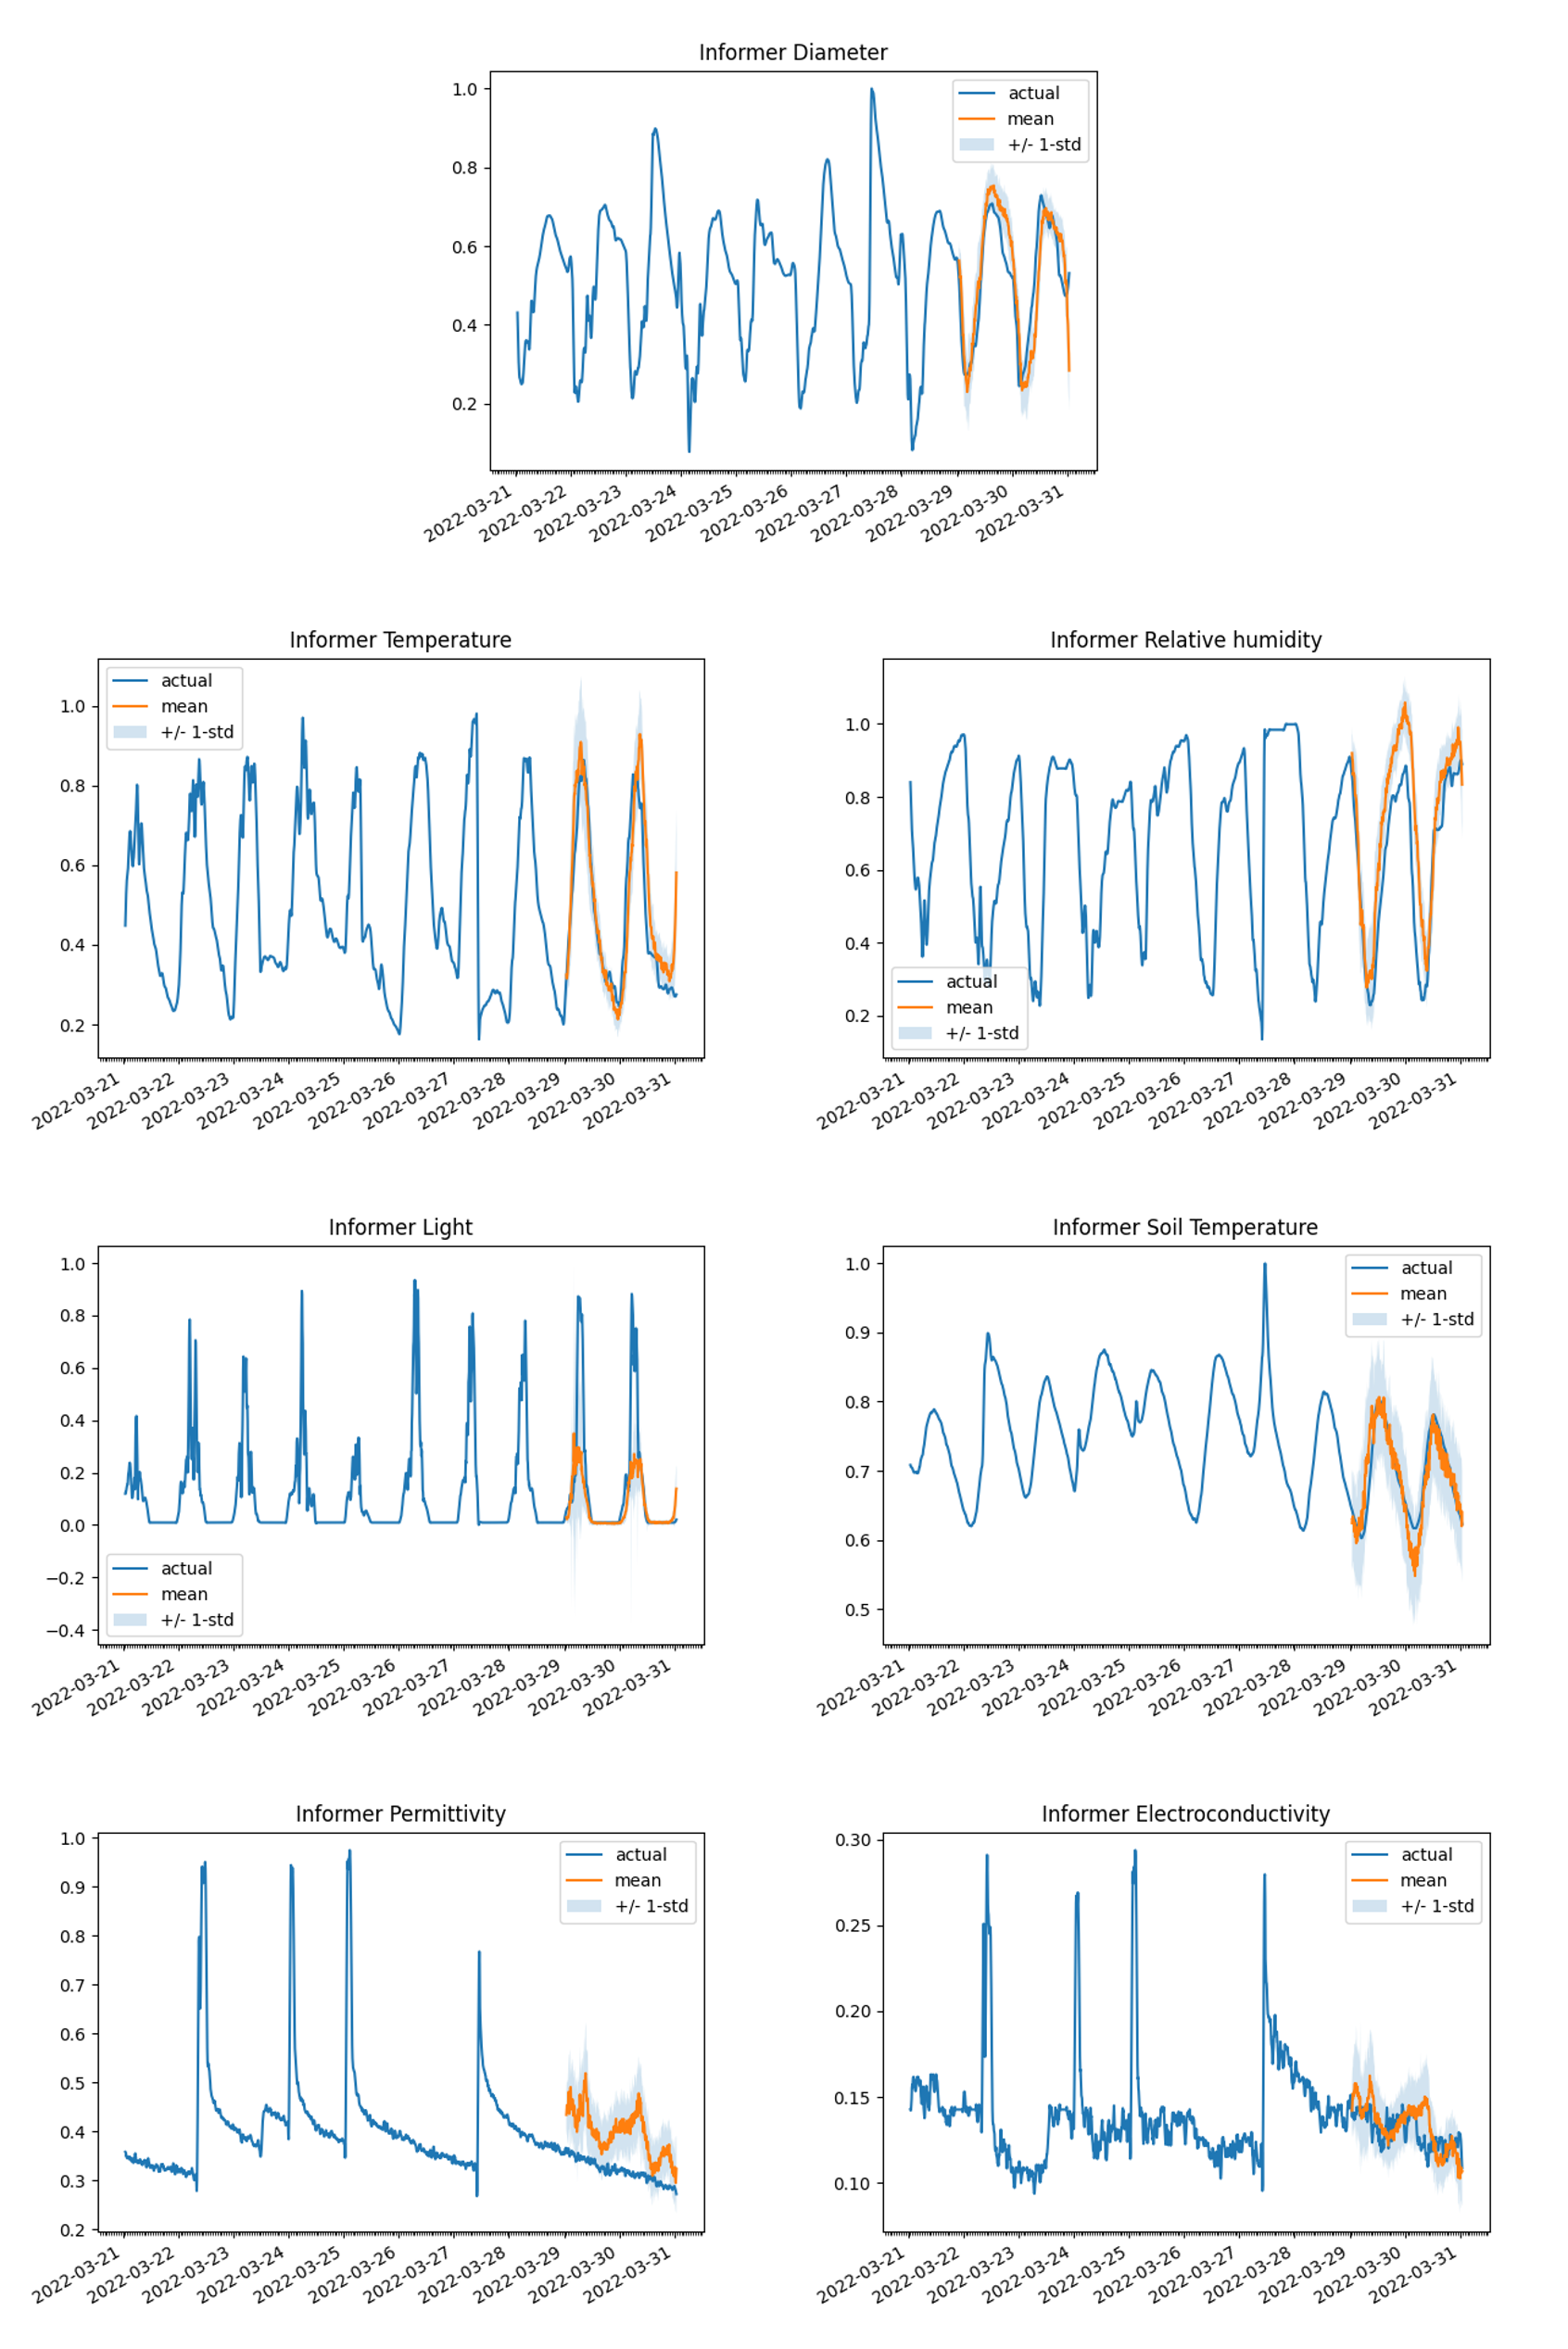
\includegraphics[width=15 cm]{6_ChapterResults/figuras/I30.png}
    \caption{Comparison between the predicted values generated by the I30 model and the actual observed values for the 7 variables over a two-day prediction horizon}
    \label{I30}
\end{figure}

\subsection{Autoformer}
The results for the Autoformer variant with modified Batch Size and Number of Epochs, as shown in Tables \ref{A5_M} and \ref{A5_R}, exhibit varied outcomes compared to the A21 model, which served as the baseline for this experimental phase. In this case, the modifications did not lead to significant improvements over the previous models.

The A29 model, recognized as one of the best outcomes in this phase, has shown significant predictive capability. This is evident in Figure \ref{A29}, where a comparison between the model's predictions and the actual values for the seven variables is presented, highlighting its superior performance.

However, as observed in Table \ref{A5_T}, similar to the results with Transformers and Informers, increasing the Batch Size and Number of Epochs results in higher computational costs and, consequently, longer training times. This highlights the trade-off between potentially better performance and increased computational demands when adjusting these hyperparameters.
    


\begin{table}[]
    \centering
    \resizebox{\textwidth}{!}{%
    \begin{tabular}{ccccccccc}
    \multicolumn{9}{c}{\textbf{MSE   (Sorted by model)}}                                                                                                                                                                                                                          \\
    Model & Diameter                       & Electroconductivity            & Light                          & Permittivity                   & Relative\_humidity             & Soil\_Temperature              & Temperature                    & Mean                           \\
    A25   & \cellcolor[HTML]{FB9073}-19.10 & \cellcolor[HTML]{63BE7B}-39.74 & \cellcolor[HTML]{F8696B}-11.07 & \cellcolor[HTML]{FCA878}-20.41 & \cellcolor[HTML]{FFE683}-16.46 & \cellcolor[HTML]{FCA276}-16.73 & \cellcolor[HTML]{FCB37A}-17.69 & \cellcolor[HTML]{FCB279}-20.17 \\
    A26   & \cellcolor[HTML]{F7E883}-21.55 & \cellcolor[HTML]{FBE983}-38.41 & \cellcolor[HTML]{FDC67D}-11.16 & \cellcolor[HTML]{FEEA83}-21.47 & \cellcolor[HTML]{E1E282}-17.06 & \cellcolor[HTML]{63BE7B}-21.72 & \cellcolor[HTML]{63BE7B}-23.03 & \cellcolor[HTML]{A2D07E}-22.06 \\
    A27   & \cellcolor[HTML]{FFE884}-21.39 & \cellcolor[HTML]{FCAA78}-36.98 & \cellcolor[HTML]{63BE7B}-11.34 & \cellcolor[HTML]{63BE7B}-28.37 & \cellcolor[HTML]{FED17F}-15.40 & \cellcolor[HTML]{F8696B}-15.05 & \cellcolor[HTML]{91CB7D}-22.38 & \cellcolor[HTML]{FFEA84}-21.56 \\
    A28   & \cellcolor[HTML]{F8696B}-18.12 & \cellcolor[HTML]{F8696B}-35.60 & \cellcolor[HTML]{FFDC81}-11.18 & \cellcolor[HTML]{F8696B}-19.47 & \cellcolor[HTML]{F8696B}-9.98  & \cellcolor[HTML]{91CB7D}-20.90 & \cellcolor[HTML]{F8696B}-13.50 & \cellcolor[HTML]{F8696B}-18.39 \\
    A29   & \cellcolor[HTML]{63BE7B}-23.10 & \cellcolor[HTML]{8FCA7D}-39.35 & \cellcolor[HTML]{DEE182}-11.23 & \cellcolor[HTML]{95CC7D}-26.12 & \cellcolor[HTML]{D6DF81}-17.17 & \cellcolor[HTML]{FDB57A}-17.33 & \cellcolor[HTML]{99CD7E}-22.28 & \cellcolor[HTML]{63BE7B}-22.37 \\
    A30   & \cellcolor[HTML]{C4DA80}-22.07 & \cellcolor[HTML]{FFEA84}-38.34 & \cellcolor[HTML]{EDE582}-11.21 & \cellcolor[HTML]{FFE984}-21.39 & \cellcolor[HTML]{63BE7B}-18.35 & \cellcolor[HTML]{A2D07E}-20.60 & \cellcolor[HTML]{FED380}-19.50 & \cellcolor[HTML]{F7E883}-21.64
    \end{tabular}%
    }
    \caption{Mean Squared Errors (MSE) for different Autoformer models obtained by varying the Batch Size and Number of Epochs values, sorted by model}
    \label{A5_M}
    \end{table}



    
\begin{table}[]
    \centering
    \resizebox{\textwidth}{!}{%
    \begin{tabular}{ccccccccc}
    \multicolumn{9}{c}{\textbf{R2 (Sorted by model)}}                                                                                                                                                                                                                     \\
    Model & Diameter                     & Electroconductivity           & Light                         & Permittivity                   & Relative\_humidity            & Soil\_Temperature             & Temperature                   & Mean                          \\
    A25   & \cellcolor[HTML]{FA9A74}0.45 & \cellcolor[HTML]{63BE7B}-0.31 & \cellcolor[HTML]{F8696B}-0.37 & \cellcolor[HTML]{FBAE78}-18.85 & \cellcolor[HTML]{FEE883}0.55  & \cellcolor[HTML]{FBB379}-4.64 & \cellcolor[HTML]{FDCC7E}0.57  & \cellcolor[HTML]{FA9F75}-3.23 \\
    A26   & \cellcolor[HTML]{F6E984}0.68 & \cellcolor[HTML]{FBEA84}-0.78 & \cellcolor[HTML]{FCC47C}-0.34 & \cellcolor[HTML]{FEEB84}-14.57 & \cellcolor[HTML]{DCE182}0.61  & \cellcolor[HTML]{63BE7B}-0.79 & \cellcolor[HTML]{63BE7B}0.87  & \cellcolor[HTML]{F7E984}-2.04 \\
    A27   & \cellcolor[HTML]{FEE883}0.67 & \cellcolor[HTML]{FCB479}-1.47 & \cellcolor[HTML]{63BE7B}-0.28 & \cellcolor[HTML]{63BE7B}-2.18  & \cellcolor[HTML]{FEDE81}0.43  & \cellcolor[HTML]{F8696B}-7.32 & \cellcolor[HTML]{86C87D}0.85  & \cellcolor[HTML]{95CD7E}-1.33 \\
    A28   & \cellcolor[HTML]{F8696B}0.30 & \cellcolor[HTML]{F8696B}-2.40 & \cellcolor[HTML]{FEDB80}-0.33 & \cellcolor[HTML]{F8696B}-23.65 & \cellcolor[HTML]{F8696B}-0.99 & \cellcolor[HTML]{84C87D}-1.16 & \cellcolor[HTML]{F8696B}-0.14 & \cellcolor[HTML]{F8696B}-4.05 \\
    A29   & \cellcolor[HTML]{63BE7B}0.78 & \cellcolor[HTML]{8BCA7E}-0.43 & \cellcolor[HTML]{DEE283}-0.32 & \cellcolor[HTML]{7EC67D}-4.33  & \cellcolor[HTML]{D0DE82}0.62  & \cellcolor[HTML]{FDC77D}-3.91 & \cellcolor[HTML]{8CCA7E}0.85  & \cellcolor[HTML]{63BE7B}-0.96 \\
    A30   & \cellcolor[HTML]{BFD981}0.72 & \cellcolor[HTML]{FEE983}-0.81 & \cellcolor[HTML]{EDE683}-0.32 & \cellcolor[HTML]{FEE883}-14.87 & \cellcolor[HTML]{63BE7B}0.71  & \cellcolor[HTML]{91CC7E}-1.32 & \cellcolor[HTML]{FEE182}0.71  & \cellcolor[HTML]{FEE683}-2.17
    \end{tabular}%
    }
    \caption{R-squared (R²) for different Autoformer models obtained by varying the Batch Size and Number of Epochs values, sorted by model}
    \label{A5_R}
    \end{table}



\begin{table}[]
    \begin{tabular}{ccccc}
    \multicolumn{2}{c}{\textbf{Training   Time (Sorted by model)}} &  & \multicolumn{2}{c}{\textbf{Training Time (Sorted   by training time)}} \\
    Model             & Training time {[}s{]}                      &  & Model                 & Training time {[}s{]}                          \\
    A25               & \cellcolor[HTML]{63BE7B}252.2              &  & A25                   & \cellcolor[HTML]{63BE7B}252.2                  \\
    A26               & \cellcolor[HTML]{FFE383}767.71             &  & A27                   & \cellcolor[HTML]{B2D47F}449.36                 \\
    A27               & \cellcolor[HTML]{B2D47F}449.36             &  & A29                   & \cellcolor[HTML]{CADB80}509.57                 \\
    A28               & \cellcolor[HTML]{FDBB7B}1365.26            &  & A26                   & \cellcolor[HTML]{FFE383}767.71                 \\
    A29               & \cellcolor[HTML]{CADB80}509.57             &  & A28                   & \cellcolor[HTML]{FDBB7B}1365.26                \\
    A30               & \cellcolor[HTML]{F8696B}2585.23            &  & A30                   & \cellcolor[HTML]{F8696B}2585.23               
    \end{tabular}
    \caption{Training times for different Autoformer models obtained by varying the Batch Size and Number of Epochs values, sorted by model and training time values}
    \label{A5_T}
    \end{table}

\begin{figure}[htbp]
    \centering
    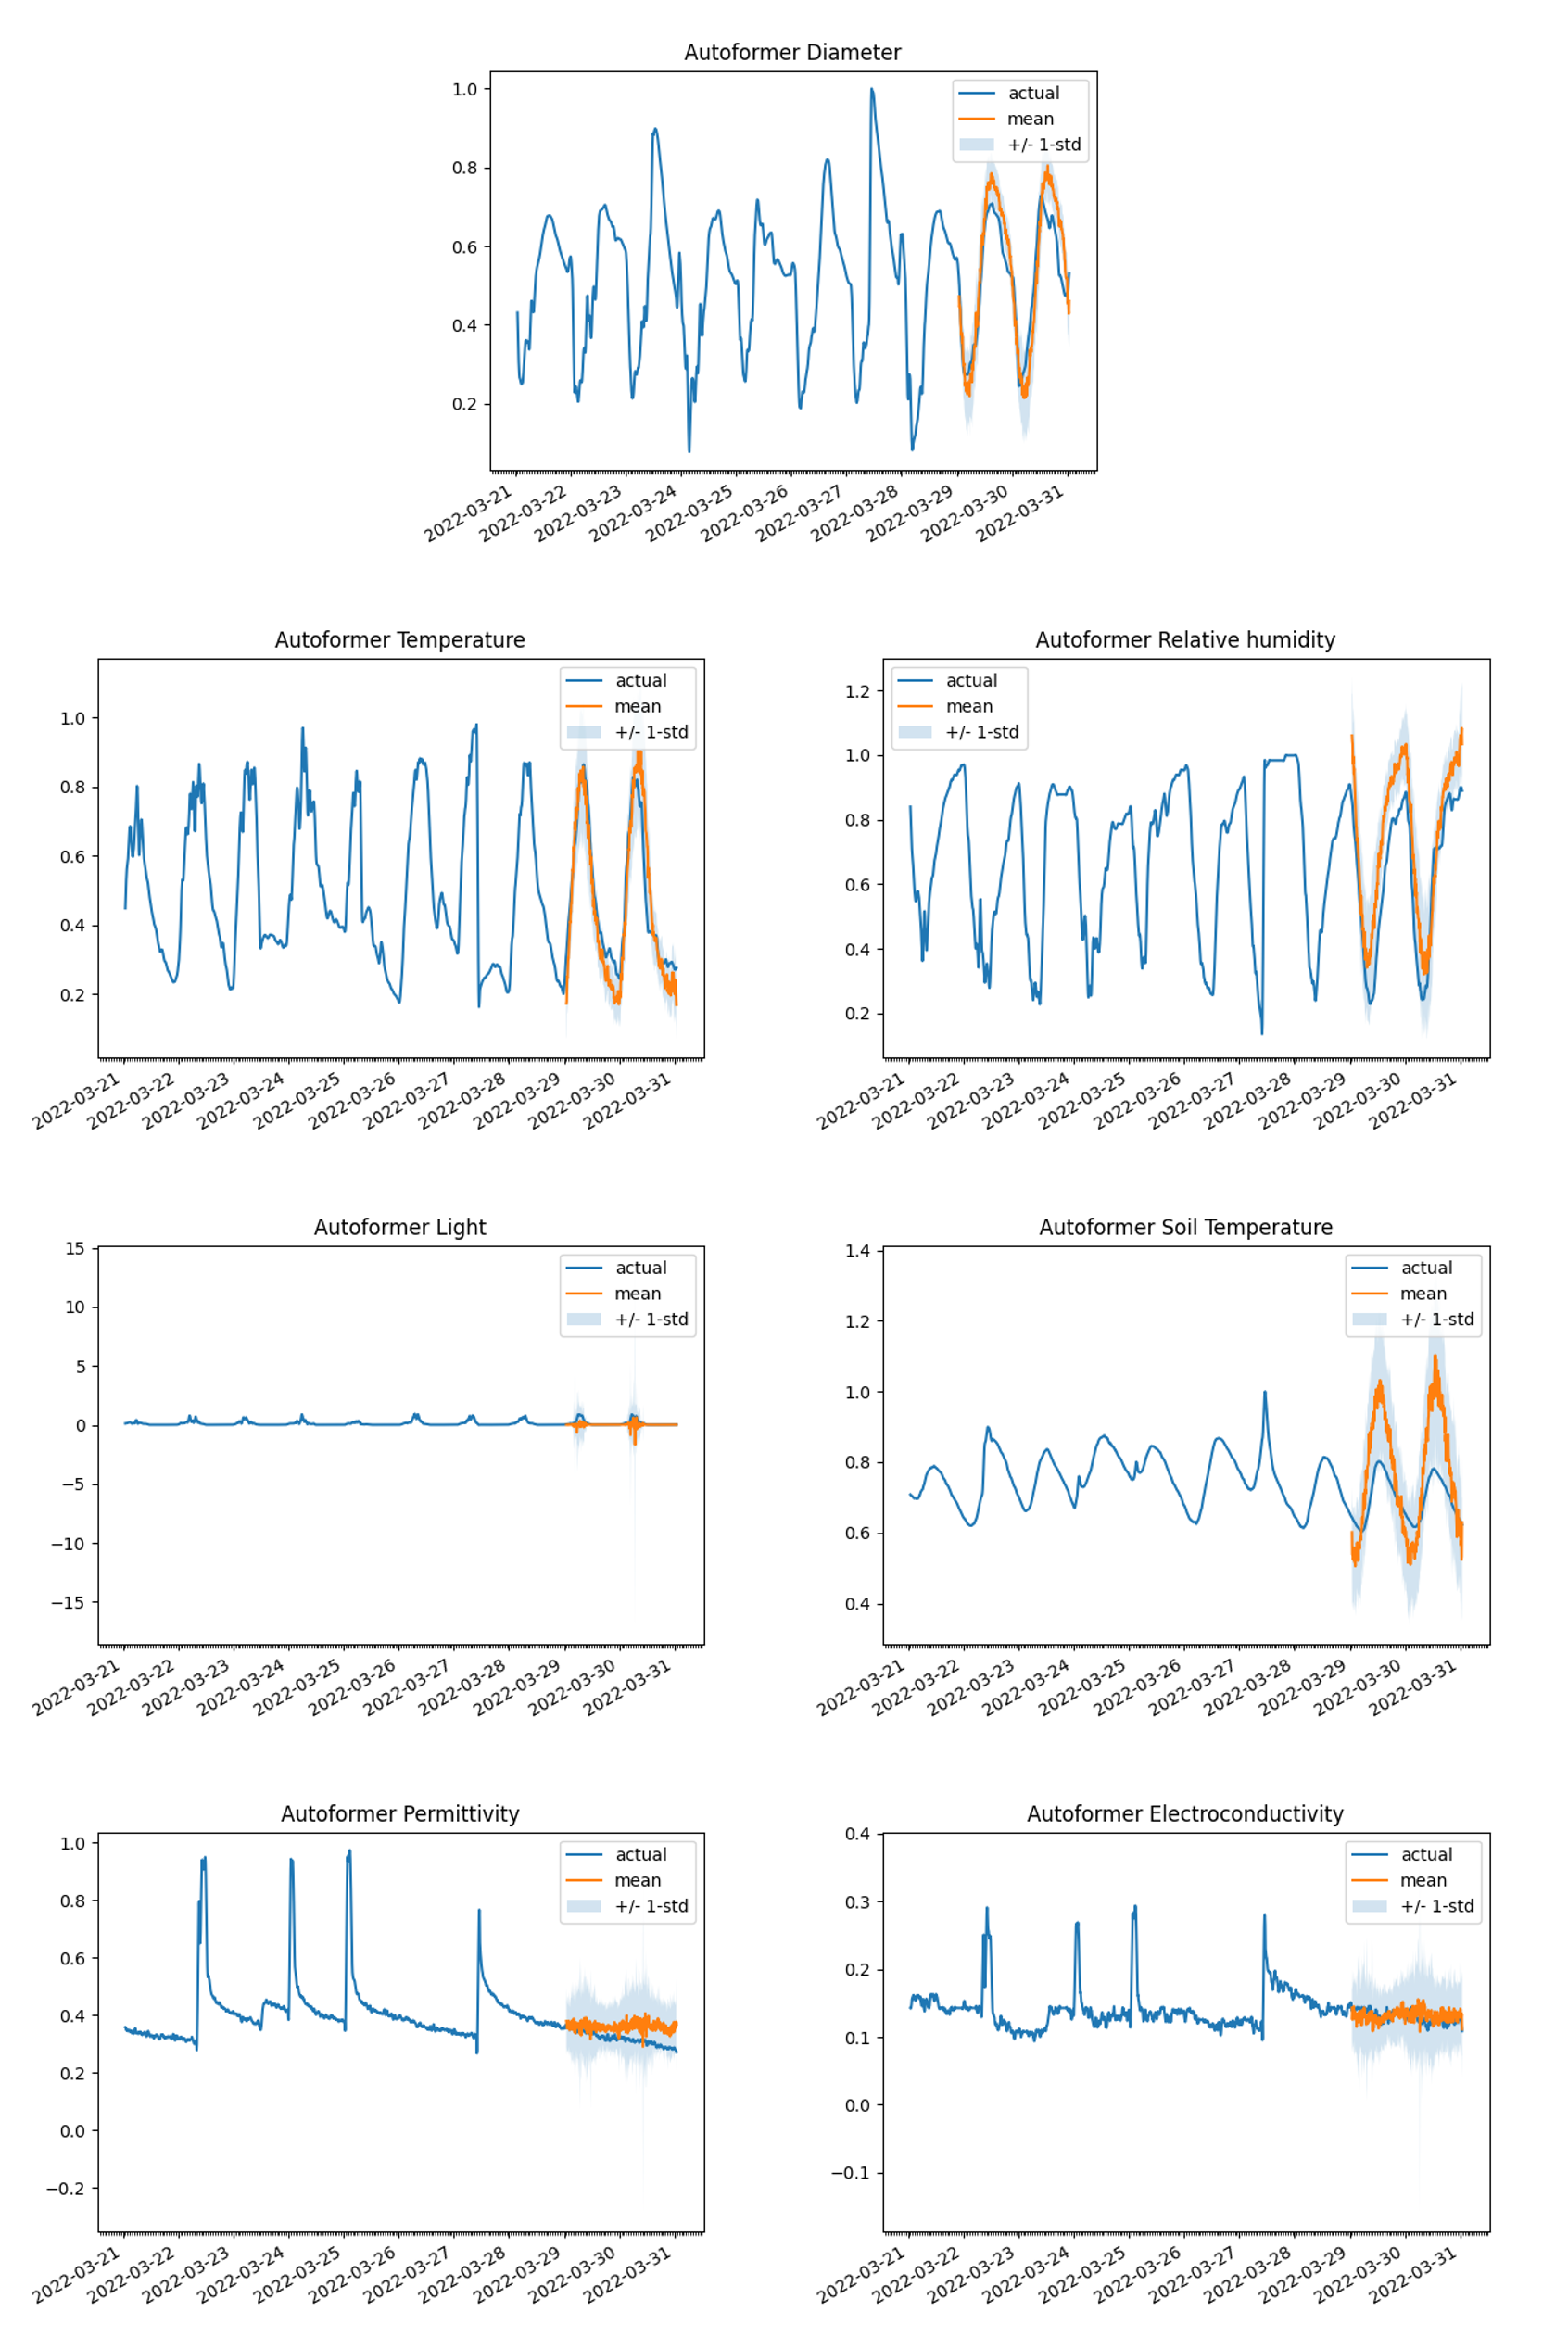
\includegraphics[width=15 cm]{6_ChapterResults/figuras/A29.png}
    \caption{Comparison between the predicted values generated by the A29 model and the actual observed values for the 7 variables over a two-day prediction horizon}
    \label{A29}
\end{figure}